\documentclass[titlepage,colorinlistoftodos]{article}
\usepackage{style}

\usepackage{float}
% \usepackage[hidelinks]{hyperref}
\usepackage{hyperref}
% \usepackage{svg}
\usepackage[inkscapeformat=png]{svg}
% \usepackage[disable]{todonotes}
\usepackage{todonotes}

\usepackage{listings}
\usepackage{xcolor}
\usepackage{pgfgantt}
\usepackage{pdflscape}
\usepackage{pgfplots} 
\usetikzlibrary{patterns}
\usepackage{changepage}

\begin{document}

\title{Implementing a Software System for Decentralized Security Risk Management}
\author{Jorn J. Verhoeven}
\birthdate{January 10th, 1995}
\birthplace{Utrecht, The Netherlands}
\defensedate{September 18th, 2023 (Estimation)}
\supervisor{Dr. Z.A. Mann}
% \committeemember{Dr. C.U. Grelck}
\maketitle

\listoftodos{}
\newpage

\tableofcontents

\asJava % By default use Java as the code language

\section*{Abstract}
With the ever growing size of \textit{the cloud} we are now, more than ever, in need of systems that can help keep our infrastructure and data safe. In this thesis we propose an implementation of a multi-agent system that is able to detect risks and negotiate on different adaptations strategies that can be autonomously applied to reduce the estimated damage. Through a software realization of the ADRIAN protocol, we show that the agents are able to keep the damage of the infrastructure at a low level, while also keeping the time spent adapting low. By running the software in a multitude of scenarios with different features enabled we can quantify the performance of the overall protocol. The implementation of, and the ADRIAN protocol itself, both have some limitations that are discussed in this thesis. But overall we believe that the ADRIAN protocol has great potential to be used in real-world scenarios.

\section{Introduction}
\label{sec:introduction}
The exponential growth of the internet has revolutionized several aspects of our modern life, such as communication, entertainment, and the way we work. Not only in the form of computers and phones, but also devices such as smart home assistants, wearables, and industrial sensors. They have enabled us to gather more data and automate many tasks, leading to increased efficiency and convenience. However, this increasing level of connectivity also brings inherent security risks and breaches \cite{khandelwal2016friday, wei2018casino}. These can have harmful effects on individuals and organizations, as they can compromise sensitive information, and cause substantial financial and reputational damage. As a result, there is a growing need for effective and possibly automated risk management and network security measures to mitigate security risks.

In a network of servers and other connected devices, it is often hard to keep track of all the possible vulnerabilities and their impact on the overall security of the network. This is especially true for IoT devices, as they are often not designed with security in mind \cite{miettinen2017iot} and are notoriously hard to update \cite{wurm2016security}. This is a problem, as these devices are often connected to the internet and can be used as a gateway to the rest of the network. 

% \comment{Zoltan}{I find it a bit strange that there is so much focus on IoT. I think the thesis is not specific to IoT}
% \comment{Zoltan}{These are valid problems, but i'm afraid the thesis will not solve them. By describing the problem, you create expectations that you will not fulfill}
% Users of smart devices such as Smart Thermometers, WiFi-connected switches, and IP Cameras are often not aware of any security vulnerabilities and their impact on their privacy and security. Where the online presence of users is receiving more and more focus these days, in the form of Multi-Factor Authentication and strong random passwords through the aid of Password Managers, IoT devices are still seemingly \emph{unprotected}. Most devices have no significant security but passwords that the user never changes. This leaves them vulnerable to a plethora of attacks \cite{hamza2019detecting, paudel2019detecting}. 

Most servers and hardware components have effective firewall settings and security measures, which significantly reduce the potential for unauthorized network access. However, it is important to note that not all devices have settings to prohibit devices from communicating with one another within the same network. Even if these settings are present some of these safeguards are turned off by default. As a result, devices with inadequate protection become easy targets for attackers. In a network of connected devices, this means that the likelihood of an attacker gaining access to a single node becomes higher as vulnerable devices are added to the network.

In an effort to track known vulnerabilities, and ultimately help automate the process of risk identification, the Common Vulnerabilities and Exposures (CVEs) system was created. This list allows software vendors to use static code analysis tools to quickly and cost-effectively find vulnerable pieces of software in their products and mitigate them accordingly. 

% Vulnerabilities that are found are usually registered in the Common Vulnerabilities and Exposures (CVEs), a system for publicly known vulnerabilities. This list allows software vendors to use static code analysis tools to quickly and cost-effectively find vulnerable pieces of software in their products and mitigate them. However, smart home devices are often hard (if not impossible) for end-users to update, leaving the older devices vulnerable to attacks. Some devices have the possibility to actively trigger a firmware update, but more often than not these updates are received in plain text \cite{wurm2016security}. This makes it impossible to guarantee that a smart home device stays secure over time.

In recent years, much research has been done into detecting security risks and intrusions within a network, specifically for IoT devices. Some researchers have investigated if machine learning could prove useful for the task of risks and intrusion detection \cite{canedo2016using, doshi2018machine, hamza2019detecting, sivanathan2018classifying}. This approach seems very accurate to a point where 99 percent of the anomalies in a network could be detected. This seems like a lot, and this accuracy on it's own is quite the achievement, but that single percent that is missing could potentially still do a lot of damage \cite{wei2018casino}. Next to that, these machine-learning models require full access to network packets to properly function which might not always be possible. These network packets would contain information such as protocol, packet size, port numbers, cipher suites, and other detailed information about the traffic. Besides leveraging the power of machine learning more research has been performed to investigate more preventative methods \cite{miettinen2017iot, hamza2019detecting, paudel2019detecting}.

Zarpelao et al. performed a survey to investigate and classify different types of intrusion detection \cite{zarpelao2017survey}. As they mention in their paper, it is not evident which method is best suited for intrusion detection in IoT Systems. This is the stepping stone through which Mann and Smolka want to enter the debate and propose another approach to the problem \cite{mann2023ADRIAN}. 
Mann and Smolka leverage a node of graphs similarly to Paudel et al. \cite{paudel2019detecting}, but instead of inspecting network traffic, they propose looking at the properties of the infrastructure. By using a set of risk rules, which are based on known CVEs, Attack Graphs are created which help to further reason about the risk of a network. More on this in Section \ref{ssec:adrian}.

This research aims to bridge the scientific knowledge gap by implementing the protocol to do \ADRIAN (ADRIAN in short). This protocol, as mentioned above, has been conceptualized by Z.A. Mann and S. Smolka \cite{mann2023ADRIAN}. This research builds upon their ideas and concepts, implementing and experimenting with a Proof of Concept (PoC) to verify and potentially suggest improvements for further research. 

\paragraph{Paper Organization}
Up till this point, we've given a brief introduction to the problem space and the research that has been done in this area. In Section \ref{sec:background} we will briefly discuss the background of this research and the concepts that are used throughout this thesis. In Section \ref{sec:methodology} we will discuss the methodology that has been used to answer the research questions. Section \ref{sec:software-realization} the overview of, and explanation of the implemented architecture will be given. Section \ref{sec:experiments} will give a detailed explanation of the executed experiments, their controls and variables. In Section \ref{sec:results} we go over the results of the experiments that have been performed. In Section \ref{sec:discussion} we will discuss the results and answer the research questions. In Section \ref{sec:conclusion} we will conclude this thesis and discuss future work.

\section{Background}
\label{sec:background}
This section will briefly mention the background of this research, and will give a summary of the ADRIAN protocol. It will also detail the components of the ADRIAN protocol that are relevant to this research.

\subsection{ADRIAN Protocol}
\label{ssec:adrian}

As mentioned in the introduction, this research builds upon the earlier work of Mann and Smolka \cite{mann2023ADRIAN}. They propose a protocol, called \ADRIAN (or ADRIAN for short), which has the core objective to identify and mitigate risks in distributed systems, leveraging a decentralized and adaptive approach. Unlike conventional security frameworks that rely on a centralized authority to oversee system security, ADRIAN empowers autonomous software agents to collaboratively assess and address security risks. An abstract representation of the ADRIAN approach is shown in Figure \ref{fig:adrian-architecture}.

\begin{figure}
    \centering
    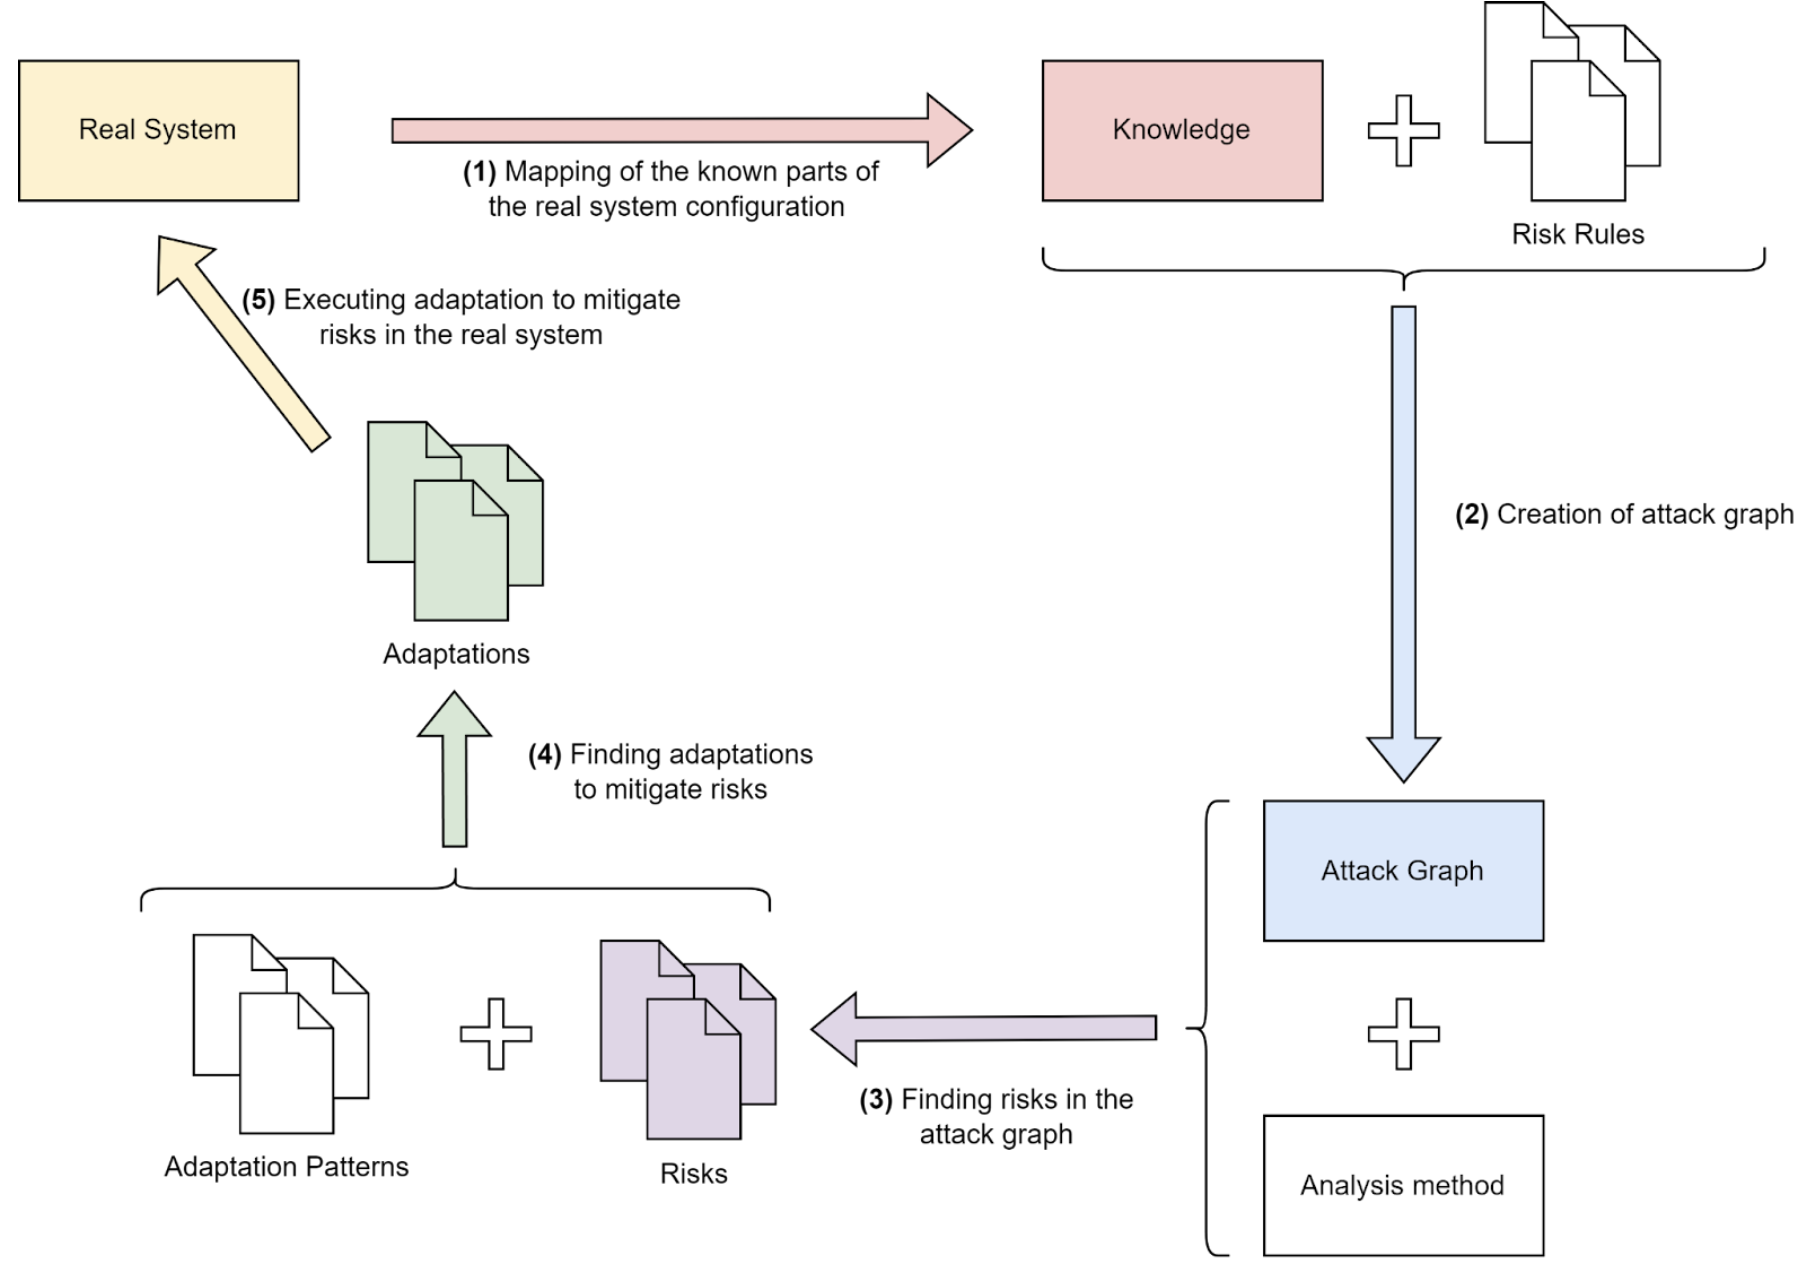
\includegraphics[width=0.8\textwidth]{content/adrian-architecture.png}
    \caption{The abstract representation of the ADRIAN approach. It shows how the different components interact with each other. This figure has been sourced from the ADRIAN concept by Mann and Smolka \cite{mann2023ADRIAN}.}
    \label{fig:adrian-architecture}
\end{figure}

In the ADRIAN protocol, agents are deployed across the infrastructure nodes of a network. These agents are responsible for monitoring the state of the node they are deployed on, specifically the properties of said node. These properties could range from firewall settings to OS and Firmware versions running on the node. Agents also know about the software that is deployed on their infrastructure node and its properties, such as SDK and software library versions, and if data is encrypted on disk. Some software components are marked as \emph{critical software}, indicating that the software contains important information or could lead to serious damage if compromised. All the information about the node and software is stored by the agent in a localized \emph{knowledge base}. Knowledge about each node, and it's software, is then exchanged between agents. This exchange will slowly propagate the knowledge throughout the network, allowing agents to have a more complete view of the network.

\vspace{0.5em}
To identify risks in a network an agent uses a set of \emph{risk rules}. These risk rules are based on known vulnerabilities, which are registered in the CVE list. They denote the probability of an attacker compromising the node/software. The definition of the risk rules that are implemented are detailed in Section \ref{ssec:risk-rules-adaptaions}.
These risk rules are then applied to the knowledge base to create \emph{attack graphs}, which are used to reason about the risk of a network. These attack graphs serve as a dynamic representation of the network's current status, where each node is represented as a vertex. Each edge ($n1 \rightarrow n2$) represents the risk that an attacker that can compromise $n1$, also manages to compromise $n2$. It is important to note that the attack graph is not an exact reflection of the real network; rather, it is a model derived from local observations and knowledge shared among agents. 
Note that sometimes vulnerabilities and risks are not yet registered as CVEs, but could exist in the real infrastructure. This means that the attack graph is not a 100\% accurate representation of the real world network, as it is not aware of these vulnerabilities. This is a problem, as it could lead to false negatives. However, this is a problem that is not unique to the ADRIAN protocol, as it is also present in other risk detection systems.

% \comment{Zoltan}{Critical software component is not explained yet.}
% \comment{Zoltan}{Risk report is not explained yet.}
% \comment{Zoltan}{Auction is not explainted yet.}
From the attack graph, agents can derive a set of \emph{critical paths}. These paths represent a path from an \emph{exposed node} to a critical software component. These critical paths are then used to determine the risk of a network and the potential damage that could be done which results in a \emph{risk report}. One of these risk reports is selected and will be \emph{auctioned} off to the agents in the network, more information about auctions is given below. In order to calculate the potential damage of a risk, the agent will combine all the probabilities of each individual edge of the attack graph along the critical path, using the following formula:

\[p = 1 - \prod_{k=1}^{R}(1-p_{k}) \]

Where $R$ is the number of all risks rules that lead to a risk edge between nodes a and b. $p_{k}$ is the probability of one of the risk rules from $R$. This formula gives us a single probability $p$ per edge. Calculating the product of all probabilities $p$ along the critical path, gets the final probability. This final probability is then multiplied with the critical software components damage (predetermined) to get the expected damage of the risk.

\vspace{0.5em}
The auctioning system is a mechanism that lets agents invite their peers to participate in the risk mitigation process. Once an agent has started an auction, other agents are invited to participate. These participating agents receive the risk report and attack graph as calculated by the initiating agent. Through a set of \emph{adaptation patterns}, agents can find multiple proposed solutions to reduce the potential damage of the risk report. These adaptation patterns are based on the risk rules, and describe possible adaptations that can be performed to mitigate the risk.
Each participating agent tries to find and select a proposal that mitigate the risk. This proposal is then sent back to the auctioneer agent, which will accumulate all proposals and select the proposal that is most beneficial to the network. The selected proposal is then executed by the agent that proposed it, and the network is updated accordingly.


\section{Methodology}
\label{sec:methodology}
The initial phase of this research involves the development and realization of a PoC implementation of the ADRIAN protocol, of which the latter is designed by Mann and Smolka in \cite{mann2023ADRIAN}. This implementation is then used to run multiple simulations in a controlled environment, which allows the collection of metrics as described in Section \ref{sec:experiments}. These metrics, of which the results are in Section \ref{sec:results}, are then used to evaluate and validate the POC implementation quantitatively. 

% \subsection{Research Approach and Design}
% \label{ssec:research-approach}
% \begin{quote}\textcolor{red}{
%     Describe the overall strategy used to tackle the problem. Is it an experimental, theoretical, or a combination of both? Explain why this approach is appropriate for the research.
% }\end{quote}

\subsection{Research Questions}
\label{ssec:research-questions}

The main research question this thesis will answer is the following question;

\vspace{0.5em}
\noindent\textbf{Research Question}\label{rq} \emph{Can the ADRIAN protocol be implemented and used for effective Risk Assessment and Mitigation?}\vspace{1em}

We envision that we can answer this overarching question by answering the following sub-questions:

\researchquestion{assessment}{(Identification) Can we use the ADRIAN protocol to do automated risk identification within a network of nodes with an (imperfect) local knowledge base? }

\researchquestion{mitigation}{(Mitigation) Can the ADRIAN protocol be used to decrease the overall risk, by applying adaptation patterns over time?}

% \subsection{Scope and Limitations}
% \label{ssec:scope-limitations}
% \begin{quote}\textcolor{red}{
%     Identify any limitations or potential sources of error in your methodology. This shows that you're aware of the constraints of your approach and helps readers interpret your results appropriately.
% }\end{quote}

\section{Software Realization}
\label{sec:software-realization}

\subsection{Overview}
\label{ssec:overview}

\subsection{Class Diagrams}
\label{ssec:class-diagrams}
\addtocontents{toc}{\protect\setcounter{tocdepth}{2}}

% Talk about:
% - To increase cohesion and reduce coupling the agent uses multiple controllers to handle the different aspects of the agent.
%   - The controllers are connected to an event bus, which is used to communicate between the controllers.
%   - The controllers are the interfacing layer between events and services that perform the actual computations.
% - The MessageBroker is used to send messages between agents.
%   - The incoming messages are handled and dispatched to the event bus, which then triggers the appropriate controller.
%   - The outgoing messages are sent to the MessageBroker, which then sends the message to the appropriate agent. In the Experimental setup there is a single message broker which is used by all agents. In a real world scenario each agent would have their own message broker, communicating over the network through HTTP or some other protocol.
% - The ExperimentalAgent is a subclass of the Agent, which is used to simulate the agents in the experimental setup, exposing the necessary methods to the ExperimentManager.
% - The ExperimentManager observes messages sent over the MessageBroker, and is able to send messages to the agents through the MessageBroker. This is helpful when measuring metrics and controlling the behavior of agents during the experiment.

% \comment{Zoltan}{I think this doesnt belonf here, but rather into a currently missing section between the current sections 3 and 4. In which you describe the design and implementation of your program. (The current section 3 contains some stubs that also belong into this to-be-created section)}
\comment{Zoltan}{It would be a good to add an overview diagram that shows the structure of the while program on a higher level of abstraction than individual classes.}
In this section, we present an overview and analysis of a UML Class Diagram for our proposed implementation of the ADRIAN protocol\cite{mann2023ADRIAN} which can be seen in Figures \ref{fig:uml-agent} through \ref{fig:uml-services}. At a quick glance the architecture features multiple controllers, connected through an internal event bus, and a message broker external communication. Additionally, some classes have been extended to support the experimental setup, which is further explained in Section \ref{sec:experiments}.

\begin{figure}[H]
    \centering
    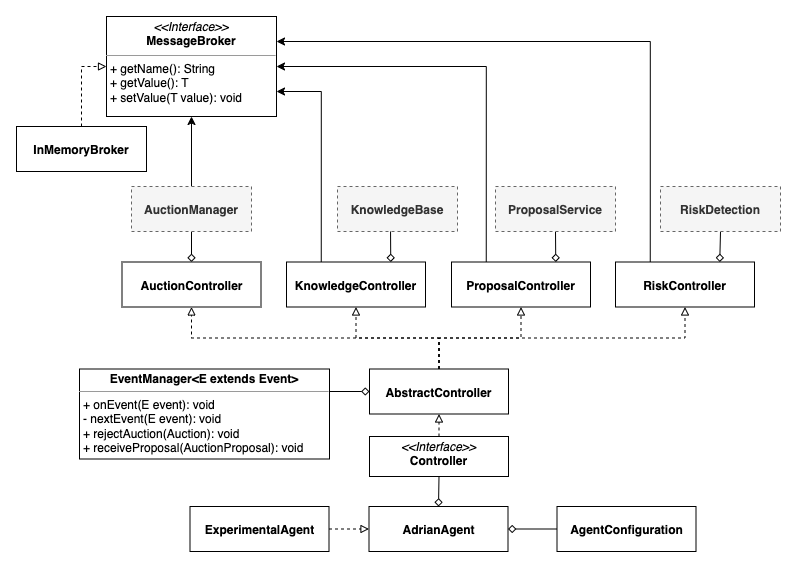
\includegraphics[width=0.8\textwidth]{_content/uml-agent}
    \caption{UML Diagram of the code structure of an Agent.}
    \label{fig:uml-agent}
\end{figure}

\subsubsection{Increased Cohesion and Reduced Coupling through Controller Interfaces}
\label{sssec:reduced-cohesion-coupling}
The systems architecture uses multiple controllers to handle various aspects of the agent, aiming to reduce both cohesion and coupling between components. Each controller is responsible for a specific set of tasks and the corresponding events, leading to a more modular and flexible design. This separation of functionality allows for easier maintenance, as well as the ability to replace controllers with new implementations, minimizing the impact on other parts of the system.
\comment{Zoltan}{Will the responsibility of each controller be described somewhere?}

\subsubsection{Event Bus for internal communication}
\label{sssec:event-bus}
To enable communication between controllers, an internal event bus is created. The event bus is in essence nothing more than a Observer pattern (also known as \texttt{EventEmitter} or \texttt{Pup/Sub}). This decouples the controllers from one another, as they are not directly aware of each other. Controllers can publish and subscribe to events on the event bus, and the event bus will then notify all subscribers when an event is published. 
\comment{Zoltan}{Should the eventbus not be visible somewhere in figure 4.}

\subsubsection{Controllers as an interfacing layer}
\label{sssec:controllers-interfacing-layer}
Controllers serve as an interfacing layer, between the event bus and the services responsible for the computations. This abstraction shields the services from the complexities of event handling, promoting modularity and reusability. It allows the services to be reused in other contexts, and makes the code easier to test as it is not dependent on any external form of communication (which is handled by the controllers).

\subsubsection{Message Broker for external communication}
\label{sssec:message-broker}
The system uses a \code{MessageBroker} which facilitates communication between agents. It allows for both incoming and outgoing messages to be handled by the agent, while abstracting away the underlying protocol. Incoming messages are processed and dispatched onto the internal event bus, triggering the relevant controllers to handle the message. On the other hand, outgoing messages are sent to the \code{MessageBroker}, which then sends the message to the appropriate agent.

The \code{MessageBroker} as an interface can be concretized by different implementations,\comment{Zoltan}{I dont understand what is meant here}depending on hardware-/software-requirements. In the experimental setup, a single \code{MessageBroker} is used by all agents and works directly in memory. This avoids any additional network complexity and allows \comment{Zoltan}{Compared to what?}a more efficient simulation. In a real world scenario, the \code{MessageBroker} would be a network service, which is used to send messages between agents over the network using HTTP requests or some other protocol such as MQTT. From the agents perspective, the \code{MessageBroker} would be the same, regardless of the implementation, and thus reducing coupling between the agents and the underlying communication protocol.

\subsubsection{Similarities in graph data structures}
\label{sssec:graph-data-structures}
In the real world the infrastructure is a graph structure, something that it \comment{Zoltan}{This could be interpreted in such a way that the speicific graph is hard-coded in the program. I think this is not what you want to say} captured in the code of the agent as well. The \code{Infrastructure}-graph consists of two types of nodes; \code{InfrastructureNode} and \code{SoftwareComponent}. These nodes can be mapped to actual hardware (e.g. Servers and IoT devices) and software (e.g. Databases and Services) in real world applications, their concrete implementation is intentionally left away in order to reduce overhead and complexity.

\begin{figure}[H]
    \centering
    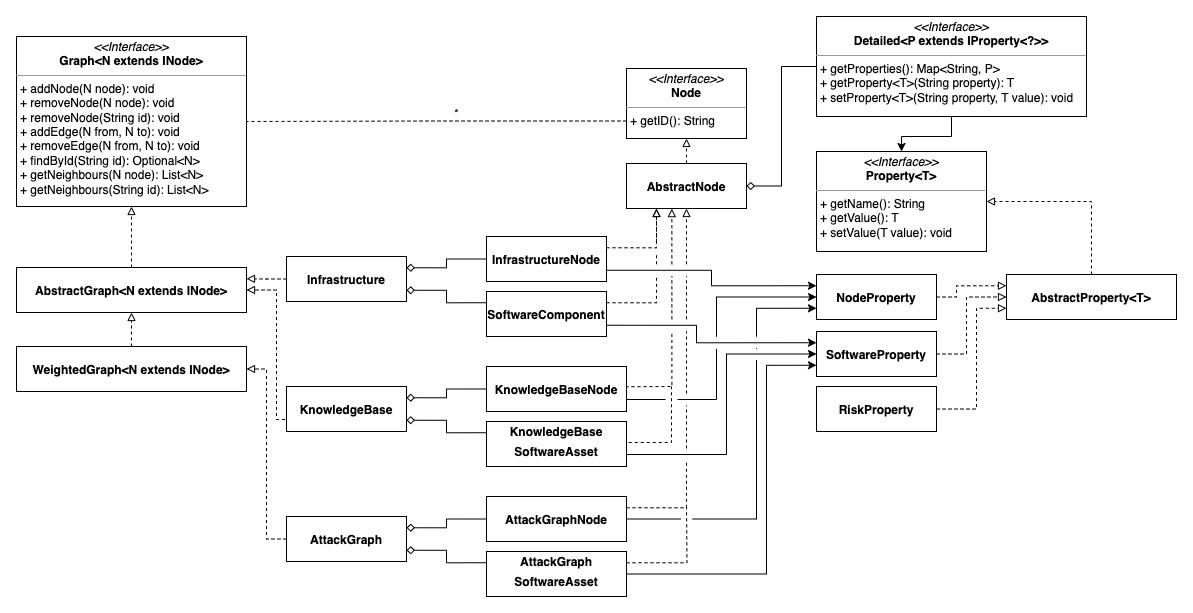
\includegraphics[width=1.2\textwidth]{_content/uml-graphs}
    \caption{UML Diagram explaining the structure of the Graphs, in a way that the separate classes are similar to their counter parts.}
    \label{fig:uml-graphs}
\end{figure}


\begin{figure}[H]
    \centering
    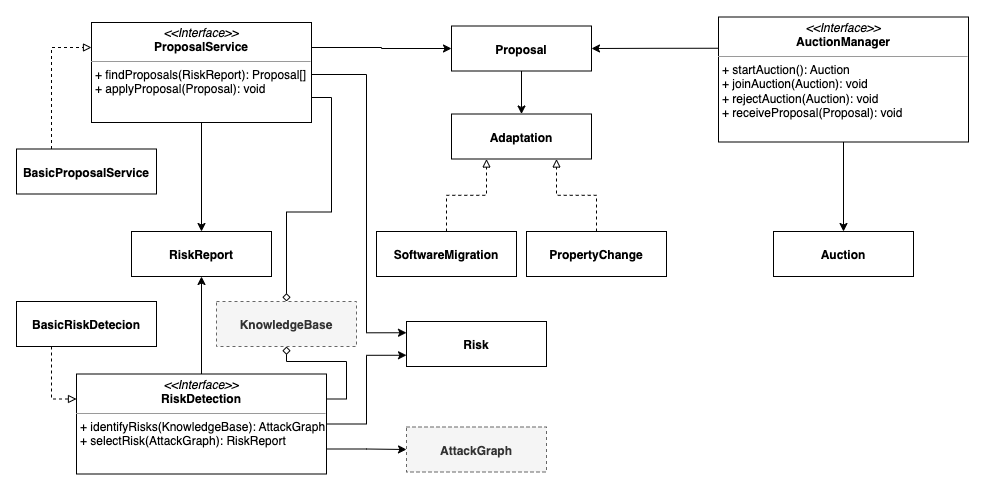
\includegraphics[width=0.8\textwidth]{_content/uml-services}
    \caption{UML Diagram depicting how the Agents services are tied together.}
    \label{fig:uml-services}
\end{figure}

\subsection{Sequence Diagrams}
\label{ssec:sequence-diagrams}
\begin{figure}[H]
    \centering
    \includegraphics[width=0.8\textwidth]{_content/knowledge-sharing}
    \caption{Knowledge Exchange Sequence Diagram}
    \label{fig:knowledge-sharing}
\end{figure}

\begin{figure}[H]
    \centering
    \includegraphics[width=0.8\textwidth]{_content/auction}
    \caption{Auction Sequence Diagram}
    \label{fig:auction}
\end{figure}

\addtocontents{toc}{\protect\setcounter{tocdepth}{3}}

\section{Experiments}
\label{sec:experiments}
To fully verify the implementation of the proposed architecture, a number of experiments have been conducted. The experiments are strategically designed to test the effect of a set of features within a specific scenario. All experiments are executed in a simulated environment, from here-on called scenario. These scenarios allow us to reproduce the experiments in a controlled and predictable environment. The feature-sets were chosen in such a way that they would individually help reason about their impact on the research questions from Subsection \ref{ssec:research-questions}. Figure \ref{fig:experiments} shows a reference of the experiments that are executed, and how the scenarios and feature-sets are combined.

\begin{figure}[H]
    \begin{adjustwidth}{-1cm}{}
        \centering
        % \begin{table}[]
        \begin{tabularx}{1.2\textwidth}{l|l|X|X|l}
            \textbf{Features \textbackslash Scenarios} & \textbf{No changess} & \textbf{Growing \newline Infrastructure} & \textbf{Unstable \newline Infrastructure} & \textbf{Mixed} \\ \hline
            \textbf{Local}                             & A.1            & A.2                    & A.3                     & A.4   \\
            \textbf{Knowledge-Sharing only}            & B.1            & B.2                    & B.3                     & B.4   \\
            \textbf{Auctioning}                        & C.1            & C.2                    & C.3                     & C.4     
        \end{tabularx}
        
    \end{adjustwidth}
    \caption{\label{fig:experiments}Overview of the experiments that are conducted. Each scenario is conducted with a different set of features, to test the effect of the features on the results.}
\end{figure}

\subsection*{Features}
Even though it would be interesting to test each feature individually, creating feature sets allowed us to focus on specific aspects of the implementation and reduce the number of experiments that needed to be conducted to a manageable number. 

The feature sets were chosen in a way that they relate to the research questions from Subsection \ref{ssec:research-questions}. The features are defined as follows:

\comment{Jorn}{I am not sure which representation to go for, either the table or the enumeration. The table is more clear in my opinion, but it feels more like a marketing thing. The enumeration is more scientific, but it is harder to read and easier to confuse maybe.}
\begin{figure}[H]
    % \begin{table}[]
        \centering
        \begin{tabular}{l|l|l|l}
            \textbf{Feature \textbackslash Set name} & \textbf{Local} & \textbf{Knowledge-Sharing} & \textbf{Auctioning} \\ \hline
            \textbf{Inspect host properties}     & yes            & yes                        & yes                 \\
            \textbf{Adapt host properties}       & yes            & yes                        & yes                 \\
            \textbf{Risk analysis}               & yes            & yes                        & yes                 \\
            \textbf{Share knowledge}             & no             & yes                        & yes                 \\
            \textbf{Initiate \& Join auctions}   & no             & no                         & yes                 \\
            \textbf{Migrate Software}            & no             & no                         & yes                            
        \end{tabular}
        \caption{\label{fig:experiment-features}Overview of the actions that are allowed in each feature set. The headers of the table represent the names of the feature sets. The rows represent the actions that are allowed in each feature set.}
    % \end{table}
\end{figure}

\begin{description}
    \item[Local*]             Agents are able to inspect, and adapt their own properties and software components. They are also allowed to do risk analysis on their knowledge base. 
    \item[Knowledge-Sharing*] Agents are able to do all of the above, and they are able to share knowledge with other agents to update their own knowledge base.
    \item[Auctioning]         Agents are able to do all of the above, and they are able to cooperate with other agents to mitigate risks through auctions. Only in this stage are agents able to join and initiate auctions.
\end{description}

{\small \textit{*The adaptations at this point only include the ability to make attribute changes. Software migrations are excluded as an agent has insufficient knowledge and capabilities to perform the migration to a node that is not its own.}}

\subsection*{Scenarios}
As mentioned before, each of the feature sets are executed in a specific scenario. A scenario is defined by an infrastructure and a set of events that will happen over time. These events could be new nodes joining the infrastructure, or nodes leaving the infrastructure. Because of the scenarios it was possible to repeat the experiments over-and-over again without having to manually change the infrastructure. This allowed for better reasoning about- and comparing the results of each individual experiment. Additionally it allowed for a more realistic approach to the experiments, as the infrastructure is not static and is changing over time.

Four scenarios have been defined, each with a different set of characteristics. These characteristics are defined as follows:

\begin{description}
    \item[No interaction]             No infrastructure changes are made overtime.
    \item[Growing Infrastructure]     The infrastructure is slowly growing over time.
    \item[Unstable Infrastructure]    Some nodes in the infrastructure are unstable and are disconnected from the network from time to time.
    \item[Mixed]                      A more realistic scenario where nodes are added and removed from the infrastructure over time.
\end{description}

\subsection{Metrics and Evaluation}
\label{ssec:metrics}
During each of the experiments a number of metrics are measured. These metrics are used to evaluate the results of the experiments and help answer the research question. 

The metrics we've defined can be categorized by effectiveness and efficiency. Effectiveness metrics measure how well the system is able to identify and mitigate risks. Efficiency metrics measure how well the system is able to do this with the least amount of resources. The metrics that are measured are shown in Figure \ref{fig:metrics-groups}.

\begin{figure}[H]
    \centering
    \begin{tabular}{l|l}
        \textbf{Effectiveness}            & \textbf{Efficiency}            \\
        Total \# of risk identified       & Total \# of messages exchanged \\
        \# of remaining risks             & \# of adaptations              \\
        Weighted sum of damages of remaining risk &                               
    \end{tabular}
    \caption{\label{fig:metrics-groups}Overview of the metrics that are measured, grouped by their category.}
\end{figure}


The metrics are defined as follows:

\begin{description}
    \item[Total number of messages exchanged] The total number of messages exchanged between agents during the epoch.
    \item[Total number of risks identified] The total number of risks identified by the agents during the epoch.
    \item[Number of remaining risks] The number of risks that have not been mitigated by the agents during the epoch.
    \item[Weighted sum of damages for remaining risks] The weighted sum of the damage for the risks that have not been mitigated by the agents during the epoch.
    % \comment{Zoltan}{I think this should be weighted by the probability of those risks}
    \item[Number of adaptations] The number of adaptations performed by the agents during the epoch.
\end{description}

\subsection{Controls and Variables}
\label{ssec:controls-variables}
% \begin{quote}\textcolor{red}{
%     Discuss any controls or variables that were taken into account to ensure the validity and reliability of your results. This could include experimental controls, randomization, and addressing potential confounding factors.
% }\end{quote}

When implementing the experiments, a number of controls and variables have been taken into account to ensure the validity and reliability of the results.

% Talk about:
% - Fake timeouts/delays
% - Knowledge sharing depth/distance

One of the things that were taken into account is the fact that for the simulation we are able to control the time that passes. This means that we are able to simulate a number of events that would take a long time in real life, in a matter of seconds. This is especially useful for the experiments where the infrastructure is growing over time. In real life, this would take a long time, but in the simulation we are able to simulate this in a matter of seconds. This allows us to test the system in a more realistic scenario, without having to wait for a long time.

There is a limit to the speed-up that can be achieved in the simulation as the processing of certain events is not instantaneous. For example, doing the risk assessment of a nodes takes time. In a real-world scenario this processing time (sub milliseconds) is negligible compared to the time messages take to travel over the network (100-1000 milliseconds) and the execution of adaptations (can take several hours to complete). However, in our simulation this processing time stays constant, and thus this processing time becomes more significant. To counter this, configurable delays were implemented to get a more realistic simulation. 
Places where these delays are implemented are for example the delivery of network-messages and the execution of adaptations. 

The second variable that can be controlled is the depth of knowledge sharing. This means that we can control how far agents are able to share their knowledge. This is done by setting a maximum distance between agents. This distance is defined as the number of hops between agents. This means that if the distance is set to 1, agents are only able to share knowledge with their direct neighbors. If the distance is set to 2, agents are able to share knowledge with their direct neighbors and the neighbors of their neighbors. This allows us to test the effect of knowledge sharing on the results of the experiments.


% \subsection{Baseline Experiment}
% % - No communication, no cooperation
% % - Predefined Infrastructure, same as other experiments
% % - Measure:
% %   - Number of adaptations
% %   - Total number of risks identified
% %   - Number of remaining risks
% %   - Sum of the damage for remaining risks

% % Mitigations take time, also communication. This should be discussed and used in the experiment.
% % Check costs of a mitigation

% \comment{Zoltan}{Arent these metrics collected in all experiments}The baseline experiment is conducted to measure metrics such as the number of adaptations and the number of risks identified. In this experiment Agents are not able to communicate with each other, and are not able to cooperate. 

% When the experiment has started, the agents are allowed to adapt their own properties and software components. However, the agents are not able to share knowledge and otherwise communicate with each other. To make the experiment easier to manage the \code{ExperimentManager} still is able to send messages to the agents, but the agents are not able to send messages to each other. \comment{Zoltan}{and also not able to cooperatively discover risks that require a global view I guess} Agents to being able to cooperate means that they are not able to join in auctions and therefore not able to work together to mitigate risks. A schematic overview of the experiment is shown in Figure \ref{fig:baseline}.

% \begin{figure}[H]
%     \centering
%     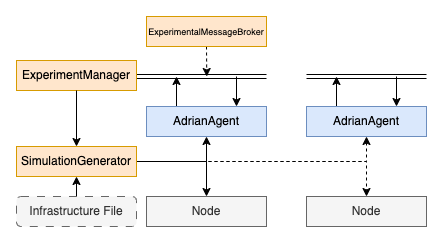
\includegraphics[width=0.8\textwidth]{_content/adrian-experiment-0}
%     \caption{Schematic overview of the baseline experiment, where multiple Agents are disconnected from one another.}
%     \label{fig:baseline}
% \end{figure}
% \comment{Zoltan}{It's not fully clear what this figure conveys. What do the individual symbols mean? In general, it is a good idea to explain all figures in the text, because they are often not as self-explanatory as you might think.}

% \subsection{Experiment 1: Risk Analysis}
% % - Communication, no cooperation
% % - Predefined Infrastructure, same as other experiments
% % - Measure:
% %   - Number of adaptations
% %   - Total number of messages exchanged
% %   - Total number of risks identified
% %   - Number of remaining risks
% %   - Sum of the damage for remaining risks

% The first experiment is conducted to measure the effect of communication between agents. In this experiment agents are able to communicate with each other, \comment{Zoltan}{I think you mean this only for mitigation, not for risk identification?} but are not able to cooperate. 

% When the experiment has started, the agents are allowed to adapt their own properties and software components. The agents are also able to share knowledge at a distance of \( D_{knowledge} \). In this experiment Agents are still not able to cooperate on mitigating risks, which is achieved by not allowing Agents to initiate or join auctions. A simplified overview of the experiment is shown in Figure \ref{fig:experiment-1}.

% \begin{figure}[H]
%     \centering
%     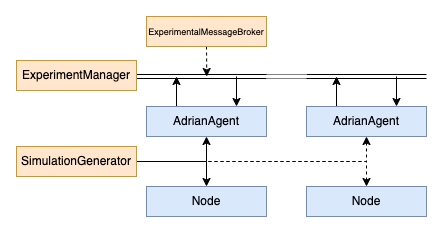
\includegraphics[width=0.8\textwidth]{_content/adrian-experiment-1}
%     \caption{Schematic overview of the first and second experiment, depicting the way multiple Agents are connected to each other and are controlled by the \code{ExperimentManager}.}
%     \label{fig:experiment-1}
% \end{figure}
% \comment{Zoltan}{It's not easy to spot the difference between this and the previous figure, like in a puzzle. Please make the life of your readers easier.}

% This experiment is repeated multiple times, with different values for \( D_{knowledge} \). The values for \( D_{knowledge} \) are 1, 2, and 3. The results of this experiment are compared to the results of the baseline experiment.

% \subsection{Experiment 2: Risk Mitigation}
% % - Communication, cooperation
% % - Predefined Infrastructure, same as other experiments
% % - Measure:
% %   - Number of adaptations
% %   - Total number of messages exchanged
% %   - Total number of risks identified
% %   - Number of remaining risks
% %   - Sum of the damage for remaining risks

% The second experiment is conducted to measure the effect of cooperation between agents. In this experiment agents are able to communicate with each other, and are able to cooperate. 

% When the experiment has started, the agents are allowed to adapt their own properties and software components. The agents are also able to share knowledge at a distance of \( D_{knowledge} \). Additionally, in this experiment Agents are able to cooperate on mitigating risks, which is achieved by allowing Agents to initiate and join auctions. The overview of this experiment is shown in Figure \ref{fig:experiment-1}.

% As with the first experiment, this experiment is repeated multiple times, with different values for \( D_{knowledge} \). The values for \( D_{knowledge} \) are 1, 2, and 3. The results of this experiment are compared to the results of the baseline experiment and the first experiment.
 
\section{Results}
\label{sec:results}
In this section we present the results of the experiments defined in section \ref{sec:experiments}. The results will be grouped per scenario. We start by a short summary of each scenario, followed by presenting the overall damage of the system in each of the scenarios, as it is the key indicator of the performance of the system. We then present the other metrics that we defined in section \ref{ssec:metrics}.

\subsection{Scenario 1: No Changes}
\textit{In this scenario, no external changes are made to the infrastructure. The purpose of this scenario is to see how the system behaves when no changes are made.}

To introduce the graphs and explain their significance, this subsection will delve into the graphs in more detail than in the subsequent subsections. 

\begin{figure}[H]
    \centering
    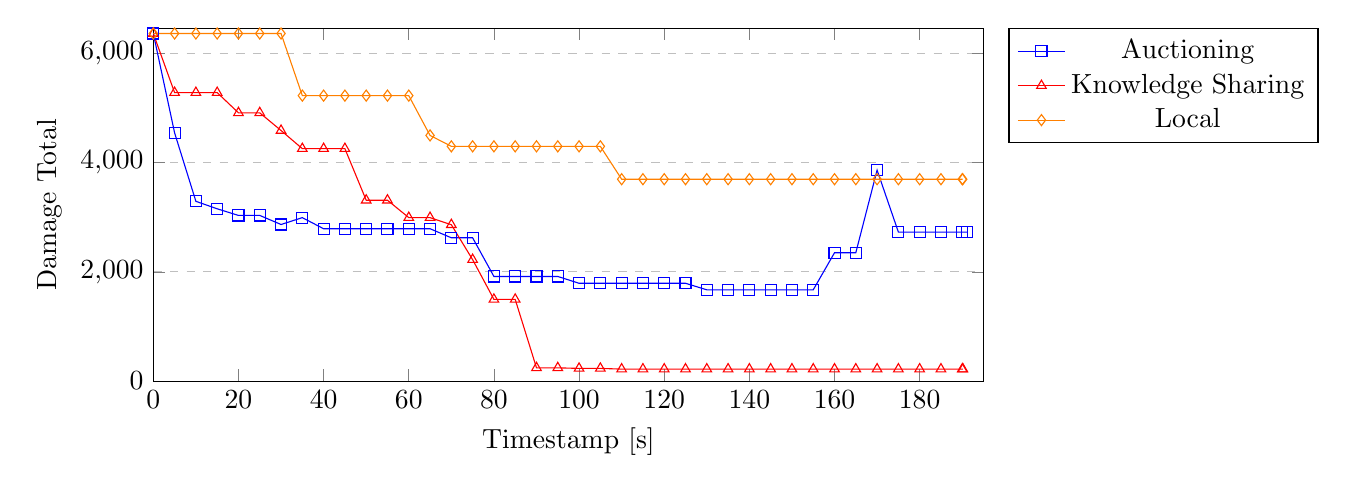
\begin{tikzpicture}
\begin{axis}[
    xlabel={Timestamp [s]},
    ylabel={Damage Total},
    xmin=0, xmax=195000,
    ymin=0, ymax=6464,
    legend pos=outer north east,
    ymajorgrids=true,
    grid style=dashed,
    width=\textwidth,
    height=0.5\textwidth,
    scaled x ticks=base 10:-3,
    xtick scale label code/.code={}
]

	\addplot[color=blue,mark=square] coordinates {
        (0,6367.26)(5000,4547.28)(10000,3293.02)(15000,3156.13)(20000,3034.57)(25000,3034.57)(30000,2868.58)(35000,2993.93)(40000,2790.80)(45000,2790.80)(50000,2790.80)(55000,2790.80)(60000,2790.80)(65000,2790.80)(70000,2624.98)(75000,2624.98)(80000,1916.52)(85000,1916.52)(90000,1916.52)(95000,1916.52)(100000,1791.72)(105000,1791.72)(110000,1791.72)(115000,1791.72)(120000,1791.72)(125000,1791.72)(130000,1671.71)(135000,1671.71)(140000,1671.71)(145000,1671.71)(150000,1671.71)(155000,1671.71)(160000,2351.16)(165000,2351.16)(170000,3864.46)(175000,2729.60)(180000,2729.60)(185000,2729.60)(190000,2729.60)(191066,2729.60)
    };
    \addlegendentry{Auctioning}
	\addplot[color=red,mark=triangle] coordinates {
        (0,6367.26)(5000,5284.52)(10000,5284.52)(15000,5284.52)(20000,4914.13)(25000,4914.13)(30000,4590.69)(35000,4257.62)(40000,4257.62)(45000,4257.62)(50000,3313.54)(55000,3313.54)(60000,2994.50)(65000,2994.50)(70000,2864.46)(75000,2224.62)(80000,1496.52)(85000,1496.52)(90000,242.72)(95000,242.72)(100000,232.18)(105000,232.18)(110000,219.25)(115000,219.25)(120000,219.25)(125000,219.25)(130000,219.25)(135000,219.25)(140000,219.25)(145000,219.25)(150000,219.25)(155000,219.25)(160000,219.25)(165000,219.25)(170000,219.25)(175000,219.25)(180000,219.25)(185000,219.25)(190000,219.25)(190155,219.25)
    };
    \addlegendentry{Knowledge Sharing}
	\addplot[color=orange,mark=diamond] coordinates {
        (0,6367.26)(5000,6367.26)(10000,6367.26)(15000,6367.26)(20000,6367.26)(25000,6367.26)(30000,6367.26)(35000,5229.23)(40000,5229.23)(45000,5229.23)(50000,5229.23)(55000,5229.23)(60000,5229.23)(65000,4499.97)(70000,4300.22)(75000,4300.22)(80000,4300.22)(85000,4300.22)(90000,4300.22)(95000,4300.22)(100000,4300.22)(105000,4300.22)(110000,3698.17)(115000,3698.17)(120000,3698.17)(125000,3698.17)(130000,3698.17)(135000,3698.17)(140000,3698.17)(145000,3698.17)(150000,3698.17)(155000,3698.17)(160000,3698.17)(165000,3698.17)(170000,3698.17)(175000,3698.17)(180000,3698.17)(185000,3698.17)(190000,3698.17)(190110,3698.17)
    };
    \addlegendentry{Local}




\end{axis}
\end{tikzpicture}
    \caption{This graph shows the overall damage of the system in the scenario where no changes are made overtime.}
    \label{fig:overall-damage-no-change}
\end{figure}

From Figure \ref{fig:overall-damage-no-change} we see that the agent with the Local-feature set (from here-on \textit{local-agent}) slowly reduces the overall damage of the network, but is unable to get any lower than around $275$, and stays at this value after roughly the first $50$ seconds.
Within the first $25$ seconds, the knowledge-sharing agents are able to reduce the overall damage to around $220$, but is unable to get any lower than this. 
Finally, the auctioning are able to reduce the damage to roughly $80$, but is only able to get there after $80$ seconds.
The lowest value is for the auctioning agent at $35\%$ of the damage the local-agent.

\begin{figure}[H]
    \centering
    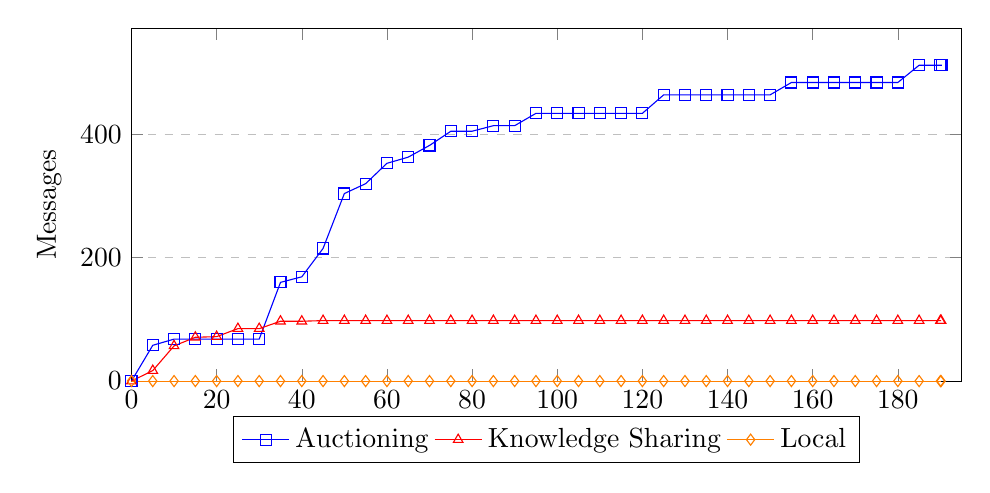
\begin{tikzpicture}
\begin{axis}[
    xlabel={Timestamp [s]},
    ylabel={Messages},
    xmin=0, xmax=195000,
    ymin=0, ymax=572,
    legend columns=-1,
    legend style={at={(0.5,-0.1)},anchor=north},
    ymajorgrids=true,
    grid style=dashed,
    width=\textwidth,
    height=0.5\textwidth,
    scaled x ticks=base 10:-3,
    xtick scale label code/.code={}
]

	\addplot[color=blue,mark=square] coordinates {
        (0,0)(5000,58)(10000,68)(15000,68)(20000,68)(25000,68)(30000,68)(35000,160)(40000,169)(45000,215)(50000,304)(55000,320)(60000,353)(65000,363)(70000,382)(75000,405)(80000,405)(85000,414)(90000,414)(95000,434)(100000,434)(105000,434)(110000,434)(115000,434)(120000,434)(125000,464)(130000,464)(135000,464)(140000,464)(145000,464)(150000,464)(155000,484)(160000,484)(165000,484)(170000,484)(175000,484)(180000,484)(185000,512)(190000,512)(190364,512)
    };
    \addlegendentry{Auctioning}
	\addplot[color=red,mark=triangle] coordinates {
        (0,0)(5000,17)(10000,57)(15000,71)(20000,72)(25000,85)(30000,85)(35000,97)(40000,97)(45000,98)(50000,98)(55000,98)(60000,98)(65000,98)(70000,98)(75000,98)(80000,98)(85000,98)(90000,98)(95000,98)(100000,98)(105000,98)(110000,98)(115000,98)(120000,98)(125000,98)(130000,98)(135000,98)(140000,98)(145000,98)(150000,98)(155000,98)(160000,98)(165000,98)(170000,98)(175000,98)(180000,98)(185000,98)(190000,98)(190165,98)
    };
    \addlegendentry{Knowledge Sharing}
	\addplot[color=orange,mark=diamond] coordinates {
        (0,0)(5000,0)(10000,0)(15000,0)(20000,0)(25000,0)(30000,0)(35000,0)(40000,0)(45000,0)(50000,0)(55000,0)(60000,0)(65000,0)(70000,0)(75000,0)(80000,0)(85000,0)(90000,0)(95000,0)(100000,0)(105000,0)(110000,0)(115000,0)(120000,0)(125000,0)(130000,0)(135000,0)(140000,0)(145000,0)(150000,0)(155000,0)(160000,0)(165000,0)(170000,0)(175000,0)(180000,0)(185000,0)(190000,0)(190150,0)
    };
    \addlegendentry{Local}




\end{axis}
\end{tikzpicture}
    \caption{Graph showing the total amount of messages sent between agents in the scenario where no changes are made overtime.}
    \label{fig:messages-no-change}
\end{figure}

In Figure \ref{fig:messages-no-change} we can see that the local-agent shares no messages, as this feature-set does not allow for it. The auctioning agent sends the most messages. After $80$ seconds all agents have found a stable point damage-wise, and this is also visible from the messages for the auctioning agents. At this point the auctioning agents have sent almost three times as much as the knowledge-sharing agents. This can be explained by the fact that the auctioning agents have a total of $11$ events that can be sent to other agents, compared to the knowledge-sharing agent, which has only $4$ types of messages. This $4 / 11$ ratio is roughly the same as the ratio between the amount of messages sent by the auctioning and knowledge-sharing agents. However, this could be a coincidence, and more research would be needed for this assumption. During an auction participating nodes send on average $4$ messages per participating node, which could also explain the difference in messages sent. 

The message count for auctioning nodes goes up roughly every $30$ second, which is the interval at which any agent will start identifying risks if it has received no messages. During this time the agents share some knowledge, sometimes start an auction but then stop because they have received no proposals, nor was able to propose any adaptations itself. 

\begin{figure}[H]
    \centering
    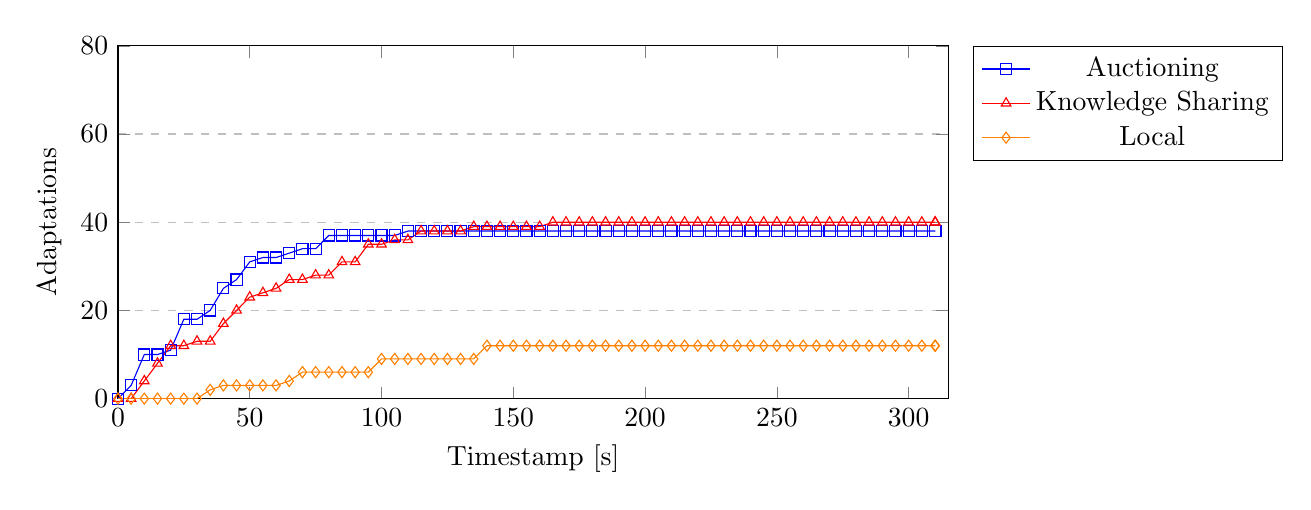
\begin{tikzpicture}
\begin{axis}[
    xlabel={Timestamp [s]},
    ylabel={Adaptations},
    xmin=0, xmax=315000,
    ymin=0, ymax=80,
    legend pos=outer north east,
    ymajorgrids=true,
    grid style=dashed,
    width=\textwidth,
    height=0.5\textwidth,
    scaled x ticks=base 10:-3,
    xtick scale label code/.code={}
]

	\addplot[color=blue,mark=square] coordinates {
        (0,0)(5000,3)(10000,10)(15000,10)(20000,11)(25000,18)(30000,18)(35000,20)(40000,25)(45000,27)(50000,31)(55000,32)(60000,32)(65000,33)(70000,34)(75000,34)(80000,37)(85000,37)(90000,37)(95000,37)(100000,37)(105000,37)(110000,38)(115000,38)(120000,38)(125000,38)(130000,38)(135000,38)(140000,38)(145000,38)(150000,38)(155000,38)(160000,38)(165000,38)(170000,38)(175000,38)(180000,38)(185000,38)(190000,38)(195000,38)(200000,38)(205000,38)(210000,38)(215000,38)(220000,38)(225000,38)(230000,38)(235000,38)(240000,38)(245000,38)(250000,38)(255000,38)(260000,38)(265000,38)(270000,38)(275000,38)(280000,38)(285000,38)(290000,38)(295000,38)(300000,38)(305000,38)(310000,38)(310169,38)
    };
    \addlegendentry{Auctioning}
	\addplot[color=red,mark=triangle] coordinates {
        (0,0)(5000,0)(10000,4)(15000,8)(20000,12)(25000,12)(30000,13)(35000,13)(40000,17)(45000,20)(50000,23)(55000,24)(60000,25)(65000,27)(70000,27)(75000,28)(80000,28)(85000,31)(90000,31)(95000,35)(100000,35)(105000,36)(110000,36)(115000,38)(120000,38)(125000,38)(130000,38)(135000,39)(140000,39)(145000,39)(150000,39)(155000,39)(160000,39)(165000,40)(170000,40)(175000,40)(180000,40)(185000,40)(190000,40)(195000,40)(200000,40)(205000,40)(210000,40)(215000,40)(220000,40)(225000,40)(230000,40)(235000,40)(240000,40)(245000,40)(250000,40)(255000,40)(260000,40)(265000,40)(270000,40)(275000,40)(280000,40)(285000,40)(290000,40)(295000,40)(300000,40)(305000,40)(310000,40)(310132,40)
    };
    \addlegendentry{Knowledge Sharing}
	\addplot[color=orange,mark=diamond] coordinates {
        (0,0)(5000,0)(10000,0)(15000,0)(20000,0)(25000,0)(30000,0)(35000,2)(40000,3)(45000,3)(50000,3)(55000,3)(60000,3)(65000,4)(70000,6)(75000,6)(80000,6)(85000,6)(90000,6)(95000,6)(100000,9)(105000,9)(110000,9)(115000,9)(120000,9)(125000,9)(130000,9)(135000,9)(140000,12)(145000,12)(150000,12)(155000,12)(160000,12)(165000,12)(170000,12)(175000,12)(180000,12)(185000,12)(190000,12)(195000,12)(200000,12)(205000,12)(210000,12)(215000,12)(220000,12)(225000,12)(230000,12)(235000,12)(240000,12)(245000,12)(250000,12)(255000,12)(260000,12)(265000,12)(270000,12)(275000,12)(280000,12)(285000,12)(290000,12)(295000,12)(300000,12)(305000,12)(310000,12)(310125,12)
    };
    \addlegendentry{Local}




\end{axis}
\end{tikzpicture}
    \caption{Graph showing the total amount of adaptations applied by agents in the scenario where no changes are made overtime.}
    \label{fig:proposals-no-change}
\end{figure}

From Figure \ref{fig:proposals-no-change} we can see that the knowledge-sharing agent applies the most adaptations, followed by the auctioning agent. The local-agent applies the least adaptations. The knowledge-sharing agent applies almost $3$ times  more adaptations than the local agent. The knowledge-sharing agent has a steep increase in the first $25$ seconds, after which it becomes more stable. The auctioning agent has a slower increase, but is applying adaptations at a steady rate. This is to be expected as any adaptation will be negotiated first, which takes time.

\begin{figure}[H]
    \centering
        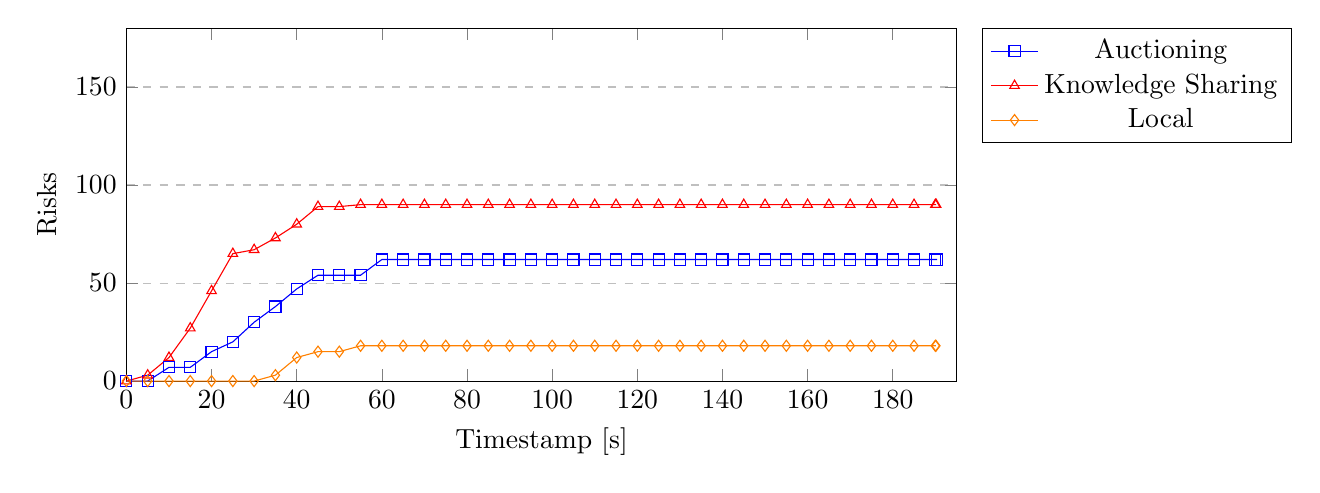
\begin{tikzpicture}
\begin{axis}[
    xlabel={Timestamp [s]},
    ylabel={Risks},
    xmin=0, xmax=195000,
    ymin=0, ymax=180,
    legend pos=outer north east,
    ymajorgrids=true,
    grid style=dashed,
    width=\textwidth,
    height=0.5\textwidth,
    scaled x ticks=base 10:-3,
    xtick scale label code/.code={}
]

	\addplot[color=blue,mark=square] coordinates {
        (0,0)(5000,0)(10000,7)(15000,7)(20000,15)(25000,20)(30000,30)(35000,38)(40000,47)(45000,54)(50000,54)(55000,54)(60000,62)(65000,62)(70000,62)(75000,62)(80000,62)(85000,62)(90000,62)(95000,62)(100000,62)(105000,62)(110000,62)(115000,62)(120000,62)(125000,62)(130000,62)(135000,62)(140000,62)(145000,62)(150000,62)(155000,62)(160000,62)(165000,62)(170000,62)(175000,62)(180000,62)(185000,62)(190000,62)(190434,62)
    };
    \addlegendentry{Auctioning}
	\addplot[color=red,mark=triangle] coordinates {
        (0,0)(5000,3)(10000,12)(15000,27)(20000,46)(25000,65)(30000,67)(35000,73)(40000,80)(45000,89)(50000,89)(55000,90)(60000,90)(65000,90)(70000,90)(75000,90)(80000,90)(85000,90)(90000,90)(95000,90)(100000,90)(105000,90)(110000,90)(115000,90)(120000,90)(125000,90)(130000,90)(135000,90)(140000,90)(145000,90)(150000,90)(155000,90)(160000,90)(165000,90)(170000,90)(175000,90)(180000,90)(185000,90)(190000,90)(190190,90)
    };
    \addlegendentry{Knowledge Sharing}
	\addplot[color=orange,mark=diamond] coordinates {
        (0,0)(5000,0)(10000,0)(15000,0)(20000,0)(25000,0)(30000,0)(35000,3)(40000,12)(45000,15)(50000,15)(55000,18)(60000,18)(65000,18)(70000,18)(75000,18)(80000,18)(85000,18)(90000,18)(95000,18)(100000,18)(105000,18)(110000,18)(115000,18)(120000,18)(125000,18)(130000,18)(135000,18)(140000,18)(145000,18)(150000,18)(155000,18)(160000,18)(165000,18)(170000,18)(175000,18)(180000,18)(185000,18)(190000,18)(190138,18)
    };
    \addlegendentry{Local}




\end{axis}
\end{tikzpicture}
    \caption{Graph showing the number of unique risks detected by agents in the scenario where no changes are made overtime.}
    \label{fig:risk-count-no-change}
\end{figure}

Figure \ref{fig:risk-count-no-change} shows that the knowledge-sharing agent detects the most risks, followed by the auctioning agent with roughly $70\%$ of the risks found. The local-agent detects the least amount of risks at only $10\%$ compared to the auctioning agent. It is to be expected that the local-agents can only detect a fraction of what the other agents detect, as the risks that can be deduced from only their local knowledge is limited.

\begin{figure}[H]
    \centering
        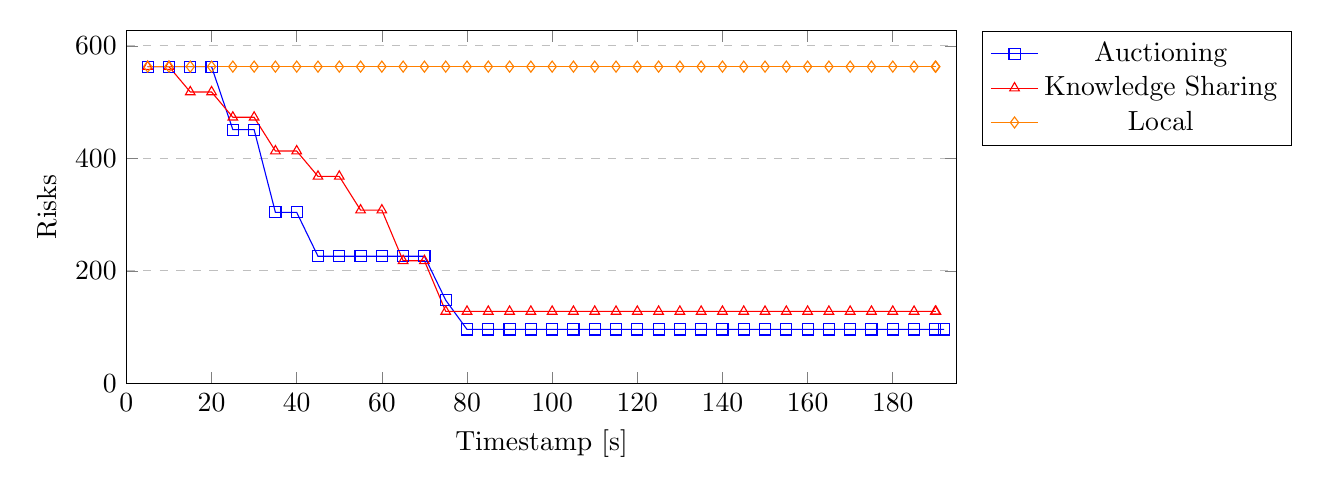
\begin{tikzpicture}
\begin{axis}[
    xlabel={Timestamp [s]},
    ylabel={Risks},
    xmin=0, xmax=195000,
    ymin=0, ymax=627,
    legend pos=outer north east,
    ymajorgrids=true,
    grid style=dashed,
    width=\textwidth,
    height=0.5\textwidth,
    scaled x ticks=base 10:-3,
    xtick scale label code/.code={}
]

	\addplot[color=blue,mark=square] coordinates {
        (5000,563)(10000,563)(15000,563)(20000,563)(25000,451)(30000,451)(35000,304)(40000,304)(45000,226)(50000,226)(55000,226)(60000,226)(65000,226)(70000,226)(75000,148)(80000,96)(85000,96)(90000,96)(95000,96)(100000,96)(105000,96)(110000,96)(115000,96)(120000,96)(125000,96)(130000,96)(135000,96)(140000,96)(145000,96)(150000,96)(155000,96)(160000,96)(165000,96)(170000,96)(175000,96)(180000,96)(185000,96)(190000,96)(192075,96)
    };
    \addlegendentry{Auctioning}
	\addplot[color=red,mark=triangle] coordinates {
        (5000,563)(10000,563)(15000,518)(20000,518)(25000,473)(30000,473)(35000,413)(40000,413)(45000,368)(50000,368)(55000,308)(60000,308)(65000,218)(70000,218)(75000,128)(80000,128)(85000,128)(90000,128)(95000,128)(100000,128)(105000,128)(110000,128)(115000,128)(120000,128)(125000,128)(130000,128)(135000,128)(140000,128)(145000,128)(150000,128)(155000,128)(160000,128)(165000,128)(170000,128)(175000,128)(180000,128)(185000,128)(190000,128)(190125,128)
    };
    \addlegendentry{Knowledge Sharing}
	\addplot[color=orange,mark=diamond] coordinates {
        (5000,563)(10000,563)(15000,563)(20000,563)(25000,563)(30000,563)(35000,563)(40000,563)(45000,563)(50000,563)(55000,563)(60000,563)(65000,563)(70000,563)(75000,563)(80000,563)(85000,563)(90000,563)(95000,563)(100000,563)(105000,563)(110000,563)(115000,563)(120000,563)(125000,563)(130000,563)(135000,563)(140000,563)(145000,563)(150000,563)(155000,563)(160000,563)(165000,563)(170000,563)(175000,563)(180000,563)(185000,563)(190000,563)(190111,563)
    };
    \addlegendentry{Local}




\end{axis}
\end{tikzpicture}
    \caption{Graph showing the number of remaining risks in the infrastructure in the scenario where no changes are made overtime.}
    \label{fig:risk-remaining-no-change}
\end{figure}

When comparing Figure \ref{fig:overall-damage-no-change} to Figure \ref{fig:risk-remaining-no-change}, we see that the graphs are following the same trend. This is to be expected, as the overall damage is calculated by summing the damage of all the remaining risks. What is interesting to see is that the auctioning agent has more remaining risks than the knowledge-sharing agent, but has a lower overall damage. 

\begin{figure}[H]
    \hspace*{-1.2cm}
    \centering
        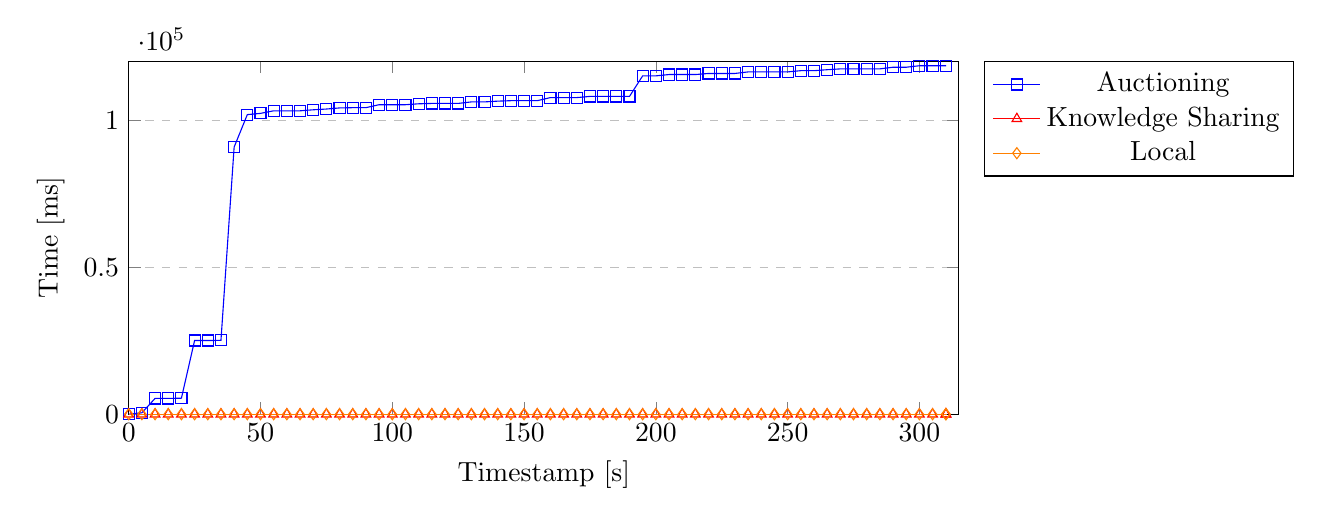
\begin{tikzpicture}
\begin{axis}[
    xlabel={Timestamp [s]},
    ylabel={Time [ms]},
    xmin=0, xmax=315000,
    ymin=0, ymax=120012,
    legend pos=outer north east,
    ymajorgrids=true,
    grid style=dashed,
    width=\textwidth,
    height=0.5\textwidth,
    scaled x ticks=base 10:-3,
    xtick scale label code/.code={}
]

	\addplot[color=blue,mark=square] coordinates {
        (0,0)(5000,475)(10000,5361)(15000,5361)(20000,5440)(25000,25066)(30000,25066)(35000,25093)(40000,90854)(45000,101889)(50000,102312)(55000,103185)(60000,103185)(65000,103185)(70000,103531)(75000,103788)(80000,104161)(85000,104251)(90000,104251)(95000,105263)(100000,105263)(105000,105263)(110000,105569)(115000,105695)(120000,105695)(125000,105695)(130000,106214)(135000,106214)(140000,106472)(145000,106629)(150000,106629)(155000,106629)(160000,107679)(165000,107679)(170000,107679)(175000,108080)(180000,108080)(185000,108080)(190000,108080)(195000,115072)(200000,115072)(205000,115518)(210000,115518)(215000,115518)(220000,115892)(225000,115892)(230000,115892)(235000,116415)(240000,116415)(245000,116415)(250000,116415)(255000,116836)(260000,116836)(265000,117162)(270000,117444)(275000,117444)(280000,117444)(285000,117444)(290000,118009)(295000,118009)(300000,118509)(305000,118509)(310000,118509)(310169,118509)
    };
    \addlegendentry{Auctioning}
	\addplot[color=red,mark=triangle] coordinates {
        (0,0)(5000,0)(10000,0)(15000,0)(20000,0)(25000,0)(30000,0)(35000,0)(40000,0)(45000,0)(50000,0)(55000,0)(60000,0)(65000,0)(70000,0)(75000,0)(80000,0)(85000,0)(90000,0)(95000,0)(100000,0)(105000,0)(110000,0)(115000,0)(120000,0)(125000,0)(130000,0)(135000,0)(140000,0)(145000,0)(150000,0)(155000,0)(160000,0)(165000,0)(170000,0)(175000,0)(180000,0)(185000,0)(190000,0)(195000,0)(200000,0)(205000,0)(210000,0)(215000,0)(220000,0)(225000,0)(230000,0)(235000,0)(240000,0)(245000,0)(250000,0)(255000,0)(260000,0)(265000,0)(270000,0)(275000,0)(280000,0)(285000,0)(290000,0)(295000,0)(300000,0)(305000,0)(310000,0)(310132,0)
    };
    \addlegendentry{Knowledge Sharing}
	\addplot[color=orange,mark=diamond] coordinates {
        (0,0)(5000,0)(10000,0)(15000,0)(20000,0)(25000,0)(30000,0)(35000,0)(40000,0)(45000,0)(50000,0)(55000,0)(60000,0)(65000,0)(70000,0)(75000,0)(80000,0)(85000,0)(90000,0)(95000,0)(100000,0)(105000,0)(110000,0)(115000,0)(120000,0)(125000,0)(130000,0)(135000,0)(140000,0)(145000,0)(150000,0)(155000,0)(160000,0)(165000,0)(170000,0)(175000,0)(180000,0)(185000,0)(190000,0)(195000,0)(200000,0)(205000,0)(210000,0)(215000,0)(220000,0)(225000,0)(230000,0)(235000,0)(240000,0)(245000,0)(250000,0)(255000,0)(260000,0)(265000,0)(270000,0)(275000,0)(280000,0)(285000,0)(290000,0)(295000,0)(300000,0)(305000,0)(310000,0)(310125,0)
    };
    \addlegendentry{Local}




\end{axis}
\end{tikzpicture}
    \caption{Graph showing the sum of time spent auctioning by agents in the scenario where no changes are made overtime.}
    \label{fig:auctioning-time-no-change}
\end{figure}

Figure \ref{fig:auctioning-time-no-change} shows that the auctioning agents is the only agent that spends time auctioning. This is to be expected, as the auctioning agents are the only agents that can auction.

\begin{figure}[H]
    \hspace*{-1.2cm}
    \centering
        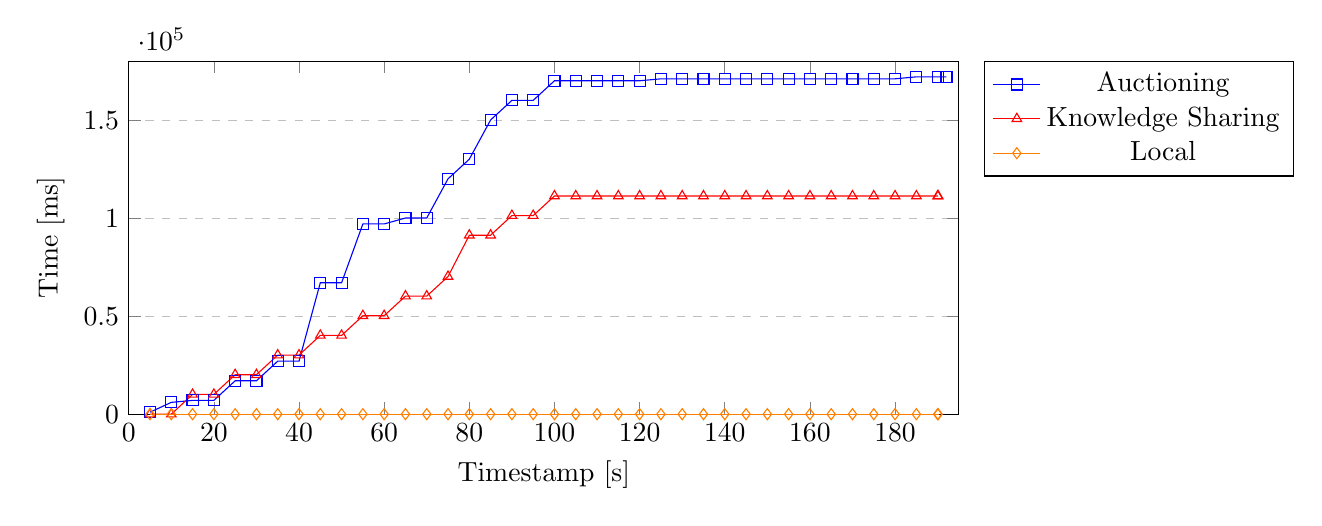
\begin{tikzpicture}
\begin{axis}[
    xlabel={Timestamp [s]},
    ylabel={Time [ms]},
    xmin=0, xmax=195000,
    ymin=0, ymax=180018,
    legend pos=outer north east,
    ymajorgrids=true,
    grid style=dashed,
    width=\textwidth,
    height=0.5\textwidth,
    scaled x ticks=base 10:-3,
    xtick scale label code/.code={}
]

	\addplot[color=blue,mark=square] coordinates {
        (5000,1004)(10000,6025)(15000,7027)(20000,7027)(25000,17033)(30000,17033)(35000,27038)(40000,27038)(45000,67055)(50000,67055)(55000,97062)(60000,97062)(65000,100075)(70000,100075)(75000,120080)(80000,130084)(85000,150091)(90000,160095)(95000,160095)(100000,170098)(105000,170098)(110000,170098)(115000,170098)(120000,170098)(125000,171100)(130000,171100)(135000,171100)(140000,171100)(145000,171100)(150000,171100)(155000,171100)(160000,171100)(165000,171100)(170000,171100)(175000,171100)(180000,171100)(185000,172103)(190000,172103)(192075,172103)
    };
    \addlegendentry{Auctioning}
	\addplot[color=red,mark=triangle] coordinates {
        (5000,0)(10000,0)(15000,10085)(20000,10085)(25000,20130)(30000,20130)(35000,30153)(40000,30153)(45000,40192)(50000,40192)(55000,50224)(60000,50224)(65000,60229)(70000,60229)(75000,70233)(80000,91314)(85000,91314)(90000,101317)(95000,101317)(100000,111324)(105000,111324)(110000,111324)(115000,111324)(120000,111324)(125000,111324)(130000,111324)(135000,111324)(140000,111324)(145000,111324)(150000,111324)(155000,111324)(160000,111324)(165000,111324)(170000,111324)(175000,111324)(180000,111324)(185000,111324)(190000,111324)(190125,111324)
    };
    \addlegendentry{Knowledge Sharing}
	\addplot[color=orange,mark=diamond] coordinates {
        (5000,0)(10000,0)(15000,0)(20000,0)(25000,0)(30000,0)(35000,0)(40000,0)(45000,0)(50000,0)(55000,0)(60000,0)(65000,0)(70000,0)(75000,0)(80000,0)(85000,0)(90000,0)(95000,0)(100000,0)(105000,0)(110000,0)(115000,0)(120000,0)(125000,0)(130000,0)(135000,0)(140000,0)(145000,0)(150000,0)(155000,0)(160000,0)(165000,0)(170000,0)(175000,0)(180000,0)(185000,0)(190000,0)(190111,0)
    };
    \addlegendentry{Local}




\end{axis}
\end{tikzpicture}
    \caption{Graph showing the sum of time spent adapting by agents in the scenario where no changes are made overtime.}
    \label{fig:adapting-time-no-change}
\end{figure}

Figure \ref{fig:adapting-time-no-change} shows that the knowledge-sharing agents spends the most amount of time adapting during this scenario. The auctioning agent is second, and the local agent spends the least amount of time adapting. This is inline with the amount of adaptations applied.

\subsection{Scenario 2: Risk Introduction}
\label{ssec:scenario-2-results}
\textit{This scenario introduces a risk to the infrastructure after $180$ seconds. The purpose of this scenario is to see how the system behaves when a new risk is introduced.}

\begin{figure}[H]
    \centering
    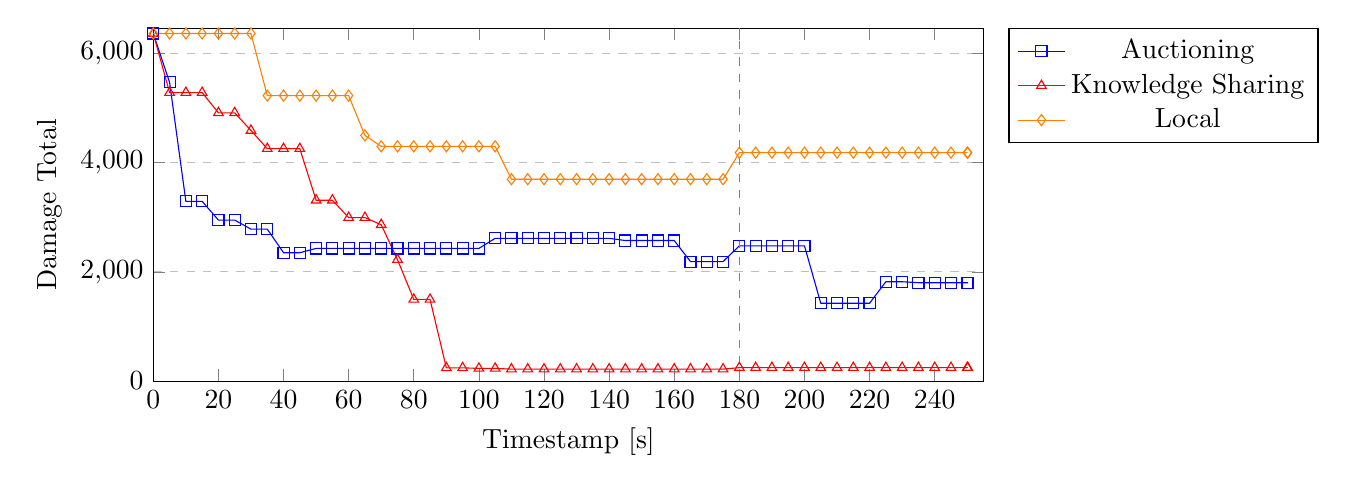
\begin{tikzpicture}
\begin{axis}[
    xlabel={Timestamp [s]},
    ylabel={Damage Total},
    xmin=0, xmax=255000,
    ymin=0, ymax=6464,
    legend pos=outer north east,
    ymajorgrids=true,
    grid style=dashed,
    width=\textwidth,
    height=0.5\textwidth,
    scaled x ticks=base 10:-3,
    xtick scale label code/.code={}
]

	\addplot[color=blue,mark=square] coordinates {
        (0,6367.26)(5000,5473.92)(10000,3293.02)(15000,3293.02)(20000,2949.34)(25000,2949.34)(30000,2783.36)(35000,2783.36)(40000,2351.49)(45000,2351.49)(50000,2430.01)(55000,2430.01)(60000,2430.01)(65000,2430.01)(70000,2430.01)(75000,2430.01)(80000,2430.01)(85000,2430.01)(90000,2430.01)(95000,2430.01)(100000,2430.01)(105000,2615.26)(110000,2615.26)(115000,2615.26)(120000,2615.26)(125000,2615.26)(130000,2615.26)(135000,2615.26)(140000,2615.26)(145000,2574.45)(150000,2574.45)(155000,2574.45)(160000,2574.45)(165000,2188.56)(170000,2188.56)(175000,2188.56)(180000,2477.58)(185000,2477.58)(190000,2477.58)(195000,2477.58)(200000,2477.58)(205000,1426.19)(210000,1426.19)(215000,1426.19)(220000,1426.19)(225000,1819.63)(230000,1819.63)(235000,1802.13)(240000,1802.13)(245000,1802.13)(250000,1802.13)(250288,1802.13)
    };
    \addlegendentry{Auctioning}
	\addplot[color=red,mark=triangle] coordinates {
        (0,6367.26)(5000,5284.52)(10000,5284.52)(15000,5284.52)(20000,4914.13)(25000,4914.13)(30000,4590.69)(35000,4257.62)(40000,4257.62)(45000,4257.62)(50000,3313.54)(55000,3313.54)(60000,2994.50)(65000,2994.50)(70000,2864.46)(75000,2224.62)(80000,1496.52)(85000,1496.52)(90000,242.72)(95000,242.72)(100000,232.18)(105000,232.18)(110000,219.25)(115000,219.25)(120000,219.25)(125000,219.25)(130000,219.25)(135000,219.25)(140000,219.25)(145000,219.25)(150000,219.25)(155000,219.25)(160000,219.25)(165000,219.25)(170000,219.25)(175000,219.25)(180000,245.68)(185000,245.68)(190000,245.68)(195000,245.68)(200000,245.68)(205000,245.68)(210000,245.68)(215000,245.68)(220000,245.68)(225000,245.68)(230000,245.68)(235000,245.68)(240000,245.68)(245000,245.68)(250000,245.68)(250159,245.68)
    };
    \addlegendentry{Knowledge Sharing}
	\addplot[color=orange,mark=diamond] coordinates {
        (0,6367.26)(5000,6367.26)(10000,6367.26)(15000,6367.26)(20000,6367.26)(25000,6367.26)(30000,6367.26)(35000,5229.23)(40000,5229.23)(45000,5229.23)(50000,5229.23)(55000,5229.23)(60000,5229.23)(65000,4499.97)(70000,4300.22)(75000,4300.22)(80000,4300.22)(85000,4300.22)(90000,4300.22)(95000,4300.22)(100000,4300.22)(105000,4300.22)(110000,3698.17)(115000,3698.17)(120000,3698.17)(125000,3698.17)(130000,3698.17)(135000,3698.17)(140000,3698.17)(145000,3698.17)(150000,3698.17)(155000,3698.17)(160000,3698.17)(165000,3698.17)(170000,3698.17)(175000,3698.17)(180000,4184.36)(185000,4184.36)(190000,4184.36)(195000,4184.36)(200000,4184.36)(205000,4184.36)(210000,4184.36)(215000,4184.36)(220000,4184.36)(225000,4184.36)(230000,4184.36)(235000,4184.36)(240000,4184.36)(245000,4184.36)(250000,4184.36)(250135,4184.36)
    };
    \addlegendentry{Local}

	\addplot[color=gray, dashed,] coordinates {(180000,0) (180000,6464)};


\end{axis}
\end{tikzpicture}
    \caption{This graph shows the overall damage of the system in the risk introduction scenario. The damage is shown for each of the three strategies. The vertical lines indicate the time at which a risk is introduced.}
    \label{fig:overall-damage-inroduce-risk}
\end{figure}

Figure \ref{fig:overall-damage-inroduce-risk} shows a graph that follows a similar trend as shown in Figure \ref{fig:overall-damage-no-change}, albeit a bit slower for the auctioning agent. This is to be expected as the scenarios are identical up until the $120$ seconds mark. During this time we see a small increase in damage for all graphs. As the metrics are collected in $5000$ms intervals, we see a small bump in all the lines around the $120$ seconds mark. And it slowly goes down again after this. Due to this timing, agents sometimes applied the adaptation before the interval ended. This explains why sometimes the lines are not as smooth as we would expect.

\begin{figure}[H]
    \centering
    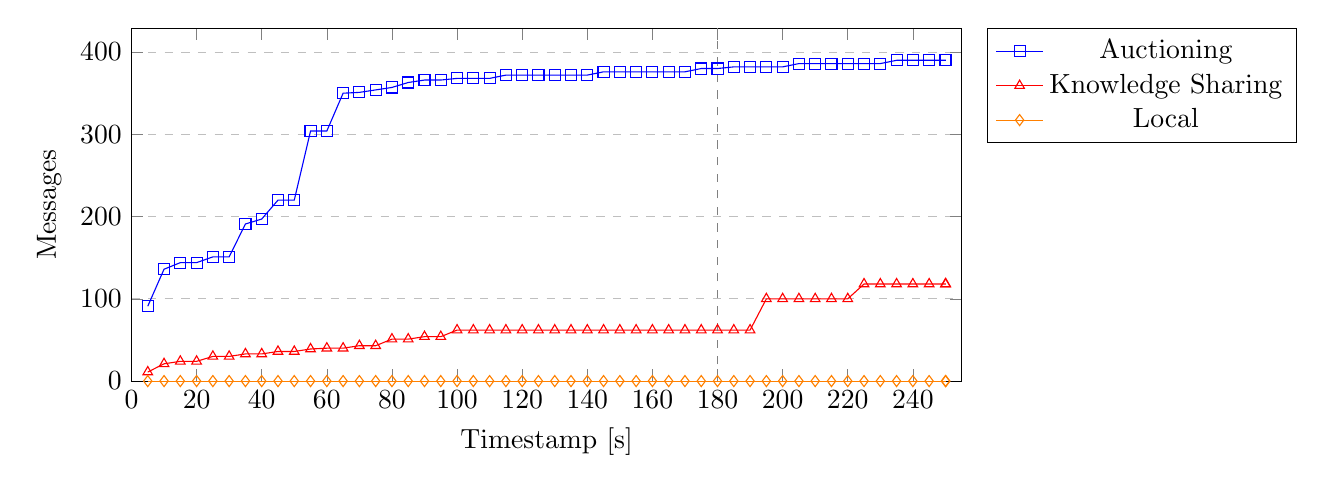
\begin{tikzpicture}
\begin{axis}[
    xlabel={Timestamp [s]},
    ylabel={Messages},
    xmin=0, xmax=255000,
    ymin=0, ymax=429,
    legend pos=outer north east,
    ymajorgrids=true,
    grid style=dashed,
    width=\textwidth,
    height=0.5\textwidth,
    scaled x ticks=base 10:-3,
    xtick scale label code/.code={}
]

	\addplot[color=blue,mark=square] coordinates {
        (5000,91)(10000,136)(15000,144)(20000,144)(25000,151)(30000,151)(35000,191)(40000,197)(45000,220)(50000,220)(55000,304)(60000,304)(65000,350)(70000,351)(75000,354)(80000,357)(85000,363)(90000,366)(95000,366)(100000,368)(105000,368)(110000,368)(115000,372)(120000,372)(125000,372)(130000,372)(135000,372)(140000,372)(145000,376)(150000,376)(155000,376)(160000,376)(165000,376)(170000,376)(175000,380)(180000,380)(185000,382)(190000,382)(195000,382)(200000,382)(205000,386)(210000,386)(215000,386)(220000,386)(225000,386)(230000,386)(235000,390)(240000,390)(245000,390)(250000,390)(250139,390)
    };
    \addlegendentry{Auctioning}
	\addplot[color=red,mark=triangle] coordinates {
        (5000,11)(10000,21)(15000,24)(20000,24)(25000,30)(30000,30)(35000,33)(40000,33)(45000,36)(50000,36)(55000,39)(60000,40)(65000,40)(70000,43)(75000,43)(80000,51)(85000,51)(90000,54)(95000,54)(100000,62)(105000,62)(110000,62)(115000,62)(120000,62)(125000,62)(130000,62)(135000,62)(140000,62)(145000,62)(150000,62)(155000,62)(160000,62)(165000,62)(170000,62)(175000,62)(180000,62)(185000,62)(190000,62)(195000,100)(200000,100)(205000,100)(210000,100)(215000,100)(220000,100)(225000,118)(230000,118)(235000,118)(240000,118)(245000,118)(250000,118)(250111,118)
    };
    \addlegendentry{Knowledge Sharing}
	\addplot[color=orange,mark=diamond] coordinates {
        (5000,0)(10000,0)(15000,0)(20000,0)(25000,0)(30000,0)(35000,0)(40000,0)(45000,0)(50000,0)(55000,0)(60000,0)(65000,0)(70000,0)(75000,0)(80000,0)(85000,0)(90000,0)(95000,0)(100000,0)(105000,0)(110000,0)(115000,0)(120000,0)(125000,0)(130000,0)(135000,0)(140000,0)(145000,0)(150000,0)(155000,0)(160000,0)(165000,0)(170000,0)(175000,0)(180000,0)(185000,0)(190000,0)(195000,0)(200000,0)(205000,0)(210000,0)(215000,0)(220000,0)(225000,0)(230000,0)(235000,0)(240000,0)(245000,0)(250000,0)(250115,0)
    };
    \addlegendentry{Local}

	\addplot[color=gray, dashed,] coordinates {(180000,0) (180000,429)};


\end{axis}
\end{tikzpicture}
    \caption{Graph showing the total amount of messages sent between agents in the risk introduction scenario.}
    \label{fig:messages-risk-introduction}
\end{figure}

Figure \ref{fig:messages-risk-introduction} shows a graph similar to Figure \ref{fig:messages-no-change}. The auctioning agent sends the most messages, followed by the knowledge-sharing agent. The local-agent sends no messages. We see that after the $120$ seconds mark, both the auctioning and knowledge-sharing agents send a few more messages around. This is to be expected as the agents detect a change in their properties, and start sharing this information with other agents.

\begin{figure}[H]
    \centering
    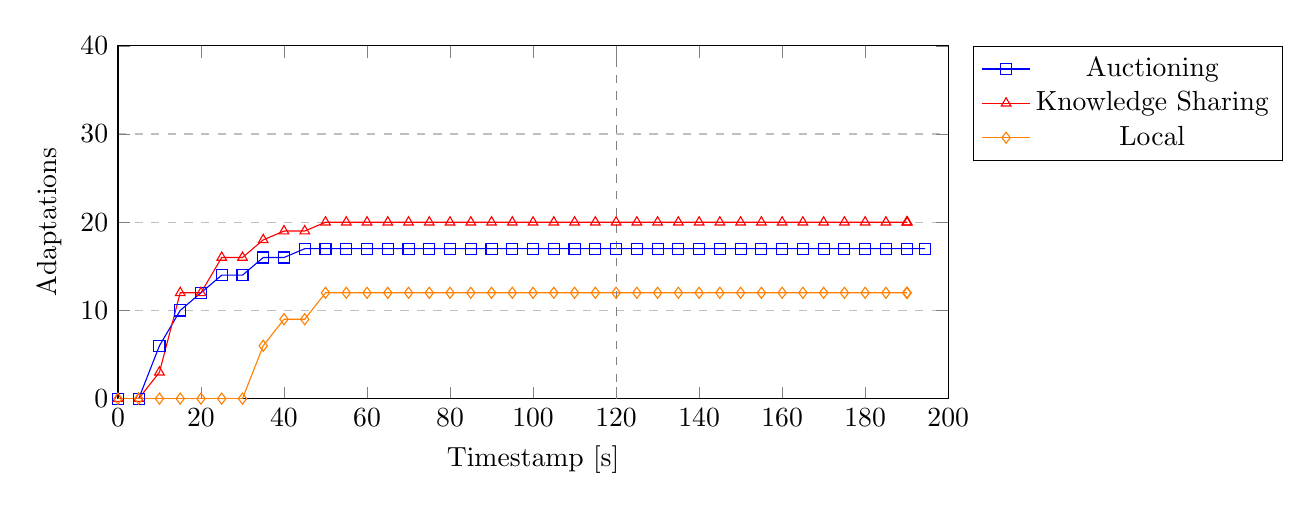
\begin{tikzpicture}
\begin{axis}[
    xlabel={Timestamp [s]},
    ylabel={Adaptations},
    xmin=0, xmax=200000,
    ymin=0, ymax=40,
    legend pos=outer north east,
    ymajorgrids=true,
    grid style=dashed,
    width=\textwidth,
    height=0.5\textwidth,
    scaled x ticks=base 10:-3,
    xtick scale label code/.code={}
]

	\addplot[color=blue,mark=square] coordinates {
        (0,0)(5000,0)(10000,6)(15000,10)(20000,12)(25000,14)(30000,14)(35000,16)(40000,16)(45000,17)(50000,17)(55000,17)(60000,17)(65000,17)(70000,17)(75000,17)(80000,17)(85000,17)(90000,17)(95000,17)(100000,17)(105000,17)(110000,17)(115000,17)(120000,17)(125000,17)(130000,17)(135000,17)(140000,17)(145000,17)(150000,17)(155000,17)(160000,17)(165000,17)(170000,17)(175000,17)(180000,17)(185000,17)(190000,17)(194444,17)
    };
    \addlegendentry{Auctioning}
	\addplot[color=red,mark=triangle] coordinates {
        (0,0)(5000,0)(10000,3)(15000,12)(20000,12)(25000,16)(30000,16)(35000,18)(40000,19)(45000,19)(50000,20)(55000,20)(60000,20)(65000,20)(70000,20)(75000,20)(80000,20)(85000,20)(90000,20)(95000,20)(100000,20)(105000,20)(110000,20)(115000,20)(120000,20)(125000,20)(130000,20)(135000,20)(140000,20)(145000,20)(150000,20)(155000,20)(160000,20)(165000,20)(170000,20)(175000,20)(180000,20)(185000,20)(190000,20)(190175,20)
    };
    \addlegendentry{Knowledge Sharing}
	\addplot[color=orange,mark=diamond] coordinates {
        (0,0)(5000,0)(10000,0)(15000,0)(20000,0)(25000,0)(30000,0)(35000,6)(40000,9)(45000,9)(50000,12)(55000,12)(60000,12)(65000,12)(70000,12)(75000,12)(80000,12)(85000,12)(90000,12)(95000,12)(100000,12)(105000,12)(110000,12)(115000,12)(120000,12)(125000,12)(130000,12)(135000,12)(140000,12)(145000,12)(150000,12)(155000,12)(160000,12)(165000,12)(170000,12)(175000,12)(180000,12)(185000,12)(190000,12)(190124,12)
    };
    \addlegendentry{Local}

	\addplot[color=gray, dashed,] coordinates {(120000,0) (120000,40)};


\end{axis}
\end{tikzpicture}
    \caption{Graph showing the total amount of adaptations applied by agents in the risk introduction scenario.}
    \label{fig:proposals-risk-introduction}
\end{figure}

When the risk is introduced after $120$ seconds, we can see in Figure \ref{fig:proposals-risk-introduction} that a few new adaptations are applied. This is in line with the damage graph in Figure \ref{fig:overall-damage-inroduce-risk}.

\begin{figure}[H]
    \centering
        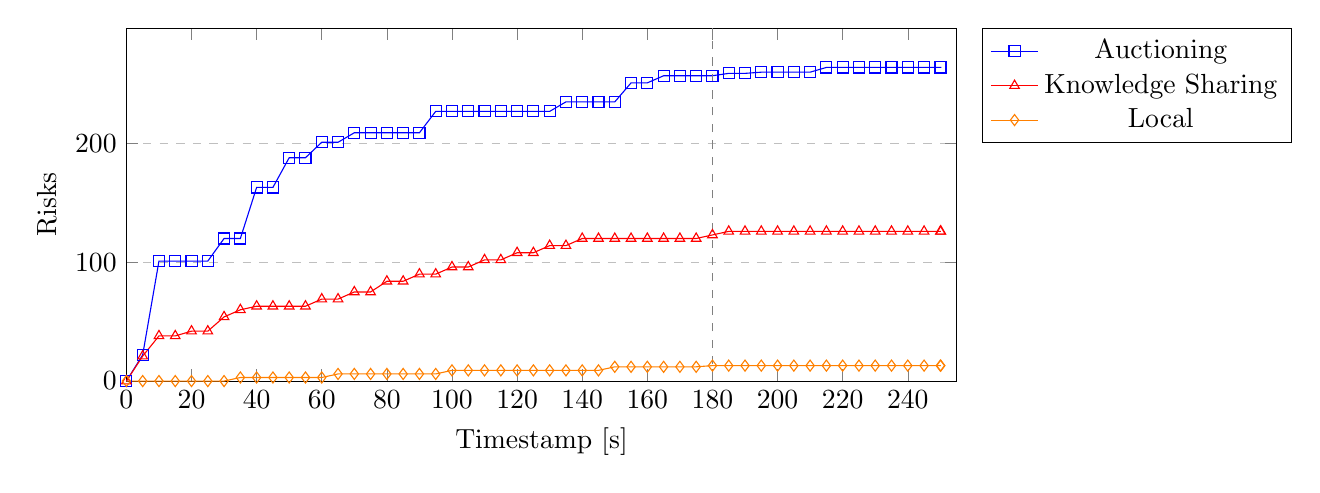
\begin{tikzpicture}
\begin{axis}[
    xlabel={Timestamp [s]},
    ylabel={Risks},
    xmin=0, xmax=255000,
    ymin=0, ymax=297,
    legend pos=outer north east,
    ymajorgrids=true,
    grid style=dashed,
    width=\textwidth,
    height=0.5\textwidth,
    scaled x ticks=base 10:-3,
    xtick scale label code/.code={}
]

	\addplot[color=blue,mark=square] coordinates {
        (0,0)(5000,22)(10000,101)(15000,101)(20000,101)(25000,101)(30000,120)(35000,120)(40000,163)(45000,163)(50000,188)(55000,188)(60000,201)(65000,201)(70000,209)(75000,209)(80000,209)(85000,209)(90000,209)(95000,227)(100000,227)(105000,227)(110000,227)(115000,227)(120000,227)(125000,227)(130000,227)(135000,235)(140000,235)(145000,235)(150000,235)(155000,251)(160000,251)(165000,257)(170000,257)(175000,257)(180000,257)(185000,259)(190000,259)(195000,260)(200000,260)(205000,260)(210000,260)(215000,264)(220000,264)(225000,264)(230000,264)(235000,264)(240000,264)(245000,264)(250000,264)(250288,264)
    };
    \addlegendentry{Auctioning}
	\addplot[color=red,mark=triangle] coordinates {
        (0,0)(5000,21)(10000,38)(15000,38)(20000,42)(25000,42)(30000,54)(35000,60)(40000,63)(45000,63)(50000,63)(55000,63)(60000,69)(65000,69)(70000,75)(75000,75)(80000,84)(85000,84)(90000,90)(95000,90)(100000,96)(105000,96)(110000,102)(115000,102)(120000,108)(125000,108)(130000,114)(135000,114)(140000,120)(145000,120)(150000,120)(155000,120)(160000,120)(165000,120)(170000,120)(175000,120)(180000,123)(185000,126)(190000,126)(195000,126)(200000,126)(205000,126)(210000,126)(215000,126)(220000,126)(225000,126)(230000,126)(235000,126)(240000,126)(245000,126)(250000,126)(250159,126)
    };
    \addlegendentry{Knowledge Sharing}
	\addplot[color=orange,mark=diamond] coordinates {
        (0,0)(5000,0)(10000,0)(15000,0)(20000,0)(25000,0)(30000,0)(35000,3)(40000,3)(45000,3)(50000,3)(55000,3)(60000,3)(65000,6)(70000,6)(75000,6)(80000,6)(85000,6)(90000,6)(95000,6)(100000,9)(105000,9)(110000,9)(115000,9)(120000,9)(125000,9)(130000,9)(135000,9)(140000,9)(145000,9)(150000,12)(155000,12)(160000,12)(165000,12)(170000,12)(175000,12)(180000,13)(185000,13)(190000,13)(195000,13)(200000,13)(205000,13)(210000,13)(215000,13)(220000,13)(225000,13)(230000,13)(235000,13)(240000,13)(245000,13)(250000,13)(250135,13)
    };
    \addlegendentry{Local}

	\addplot[color=gray, dashed,] coordinates {(180000,0) (180000,297)};


\end{axis}
\end{tikzpicture}
    \caption{Graph showing the number of unique risks detected by agents in the risk introduction scenario.}
    \label{fig:risk-count-risk-introduction}
\end{figure}

When we look at Figure \ref{fig:risk-count-risk-introduction} we can see that the knowledge-sharing agent detects the most risks, followed by the auctioning agent. The local-agent detects the least amount of risks, at only $10\%$ of the risks found by the knowledge-sharing agent. We would expect a comparable result between the auctioning and knowledge-sharing agents, however this is not the case. This is likely due to the fact that in the knowledge-sharing setup agents apply multiple adaptations in parallel. This causes the knowledge bases to change more rapidly, which could cause the agents to detect more risks. This is explained in more detail in subsection \ref{ssec:metrics}.

\begin{figure}[H]
    \centering
        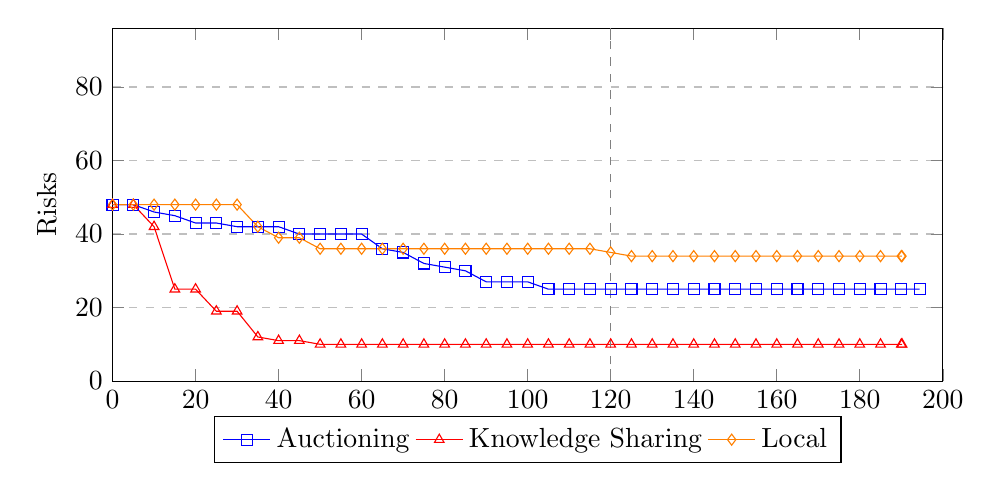
\begin{tikzpicture}
\begin{axis}[
    xlabel={Timestamp [s]},
    ylabel={Risks},
    xmin=0, xmax=200000,
    ymin=0, ymax=96,
    legend columns=-1,
    legend style={at={(0.5,-0.1)},anchor=north},
    ymajorgrids=true,
    grid style=dashed,
    width=\textwidth,
    height=0.5\textwidth,
    scaled x ticks=base 10:-3,
    xtick scale label code/.code={}
]

	\addplot[color=blue,mark=square] coordinates {
        (0,48)(5000,48)(10000,46)(15000,45)(20000,43)(25000,43)(30000,42)(35000,42)(40000,42)(45000,40)(50000,40)(55000,40)(60000,40)(65000,36)(70000,35)(75000,32)(80000,31)(85000,30)(90000,27)(95000,27)(100000,27)(105000,25)(110000,25)(115000,25)(120000,25)(125000,25)(130000,25)(135000,25)(140000,25)(145000,25)(150000,25)(155000,25)(160000,25)(165000,25)(170000,25)(175000,25)(180000,25)(185000,25)(190000,25)(194440,25)
    };
    \addlegendentry{Auctioning}
	\addplot[color=red,mark=triangle] coordinates {
        (0,48)(5000,48)(10000,42)(15000,25)(20000,25)(25000,19)(30000,19)(35000,12)(40000,11)(45000,11)(50000,10)(55000,10)(60000,10)(65000,10)(70000,10)(75000,10)(80000,10)(85000,10)(90000,10)(95000,10)(100000,10)(105000,10)(110000,10)(115000,10)(120000,10)(125000,10)(130000,10)(135000,10)(140000,10)(145000,10)(150000,10)(155000,10)(160000,10)(165000,10)(170000,10)(175000,10)(180000,10)(185000,10)(190000,10)(190192,10)
    };
    \addlegendentry{Knowledge Sharing}
	\addplot[color=orange,mark=diamond] coordinates {
        (0,48)(5000,48)(10000,48)(15000,48)(20000,48)(25000,48)(30000,48)(35000,42)(40000,39)(45000,39)(50000,36)(55000,36)(60000,36)(65000,36)(70000,36)(75000,36)(80000,36)(85000,36)(90000,36)(95000,36)(100000,36)(105000,36)(110000,36)(115000,36)(120000,35)(125000,34)(130000,34)(135000,34)(140000,34)(145000,34)(150000,34)(155000,34)(160000,34)(165000,34)(170000,34)(175000,34)(180000,34)(185000,34)(190000,34)(190162,34)
    };
    \addlegendentry{Local}

	\addplot[color=gray, dashed,] coordinates {(120000,0) (120000,96)};


\end{axis}
\end{tikzpicture}
    \caption{Graph showing the number of remaining risks in the infrastructure in the risk introduction scenario.}
    \label{fig:risk-remaining-risk-introduction}
\end{figure}

Figure \ref{fig:risk-remaining-risk-introduction} shows that the auctioning agent has more remaining risks than the knowledge-sharing agent, similar to Figure \ref{fig:risk-remaining-no-change}. At the $120$ seconds mark we would expect a small bump, as several risks are introduced, but the line stays flat. From Figure \ref{fig:risk-count-risk-introduction} we can see that these risks are actually detected by the agents. Cross referencing this with Figure \ref{fig:proposals-risk-introduction} we can see that the agents are applying adaptations to these risks, which could explain why the amount of remaining risks stays the same.

\begin{figure}[H]
    \hspace*{-1.2cm}
    \centering
        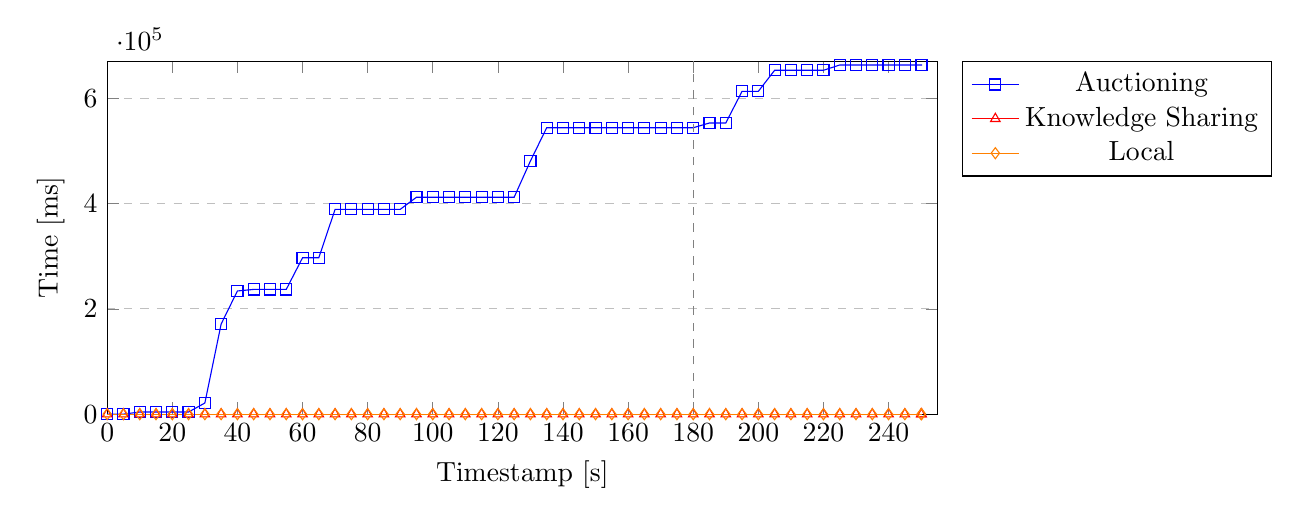
\begin{tikzpicture}
\begin{axis}[
    xlabel={Timestamp [s]},
    ylabel={Time [ms]},
    xmin=0, xmax=255000,
    ymin=0, ymax=670067,
    legend pos=outer north east,
    ymajorgrids=true,
    grid style=dashed,
    width=\textwidth,
    height=0.5\textwidth,
    scaled x ticks=base 10:-3,
    xtick scale label code/.code={}
]

	\addplot[color=blue,mark=square] coordinates {
        (0,0)(5000,64)(10000,4143)(15000,4143)(20000,4143)(25000,4143)(30000,21179)(35000,171183)(40000,233978)(45000,236929)(50000,236929)(55000,236929)(60000,297046)(65000,297049)(70000,388980)(75000,388980)(80000,388980)(85000,388980)(90000,388980)(95000,411980)(100000,411980)(105000,411980)(110000,411980)(115000,411980)(120000,411980)(125000,411980)(130000,480905)(135000,543951)(140000,543951)(145000,543951)(150000,543951)(155000,543958)(160000,543958)(165000,543962)(170000,543962)(175000,543962)(180000,543962)(185000,553054)(190000,553054)(195000,613073)(200000,613073)(205000,653079)(210000,653079)(215000,653087)(220000,653087)(225000,663101)(230000,663101)(235000,663101)(240000,663101)(245000,663101)(250000,663101)(250288,663101)
    };
    \addlegendentry{Auctioning}
	\addplot[color=red,mark=triangle] coordinates {
        (0,0)(5000,0)(10000,0)(15000,0)(20000,0)(25000,0)(30000,0)(35000,0)(40000,0)(45000,0)(50000,0)(55000,0)(60000,0)(65000,0)(70000,0)(75000,0)(80000,0)(85000,0)(90000,0)(95000,0)(100000,0)(105000,0)(110000,0)(115000,0)(120000,0)(125000,0)(130000,0)(135000,0)(140000,0)(145000,0)(150000,0)(155000,0)(160000,0)(165000,0)(170000,0)(175000,0)(180000,0)(185000,0)(190000,0)(195000,0)(200000,0)(205000,0)(210000,0)(215000,0)(220000,0)(225000,0)(230000,0)(235000,0)(240000,0)(245000,0)(250000,0)(250159,0)
    };
    \addlegendentry{Knowledge Sharing}
	\addplot[color=orange,mark=diamond] coordinates {
        (0,0)(5000,0)(10000,0)(15000,0)(20000,0)(25000,0)(30000,0)(35000,0)(40000,0)(45000,0)(50000,0)(55000,0)(60000,0)(65000,0)(70000,0)(75000,0)(80000,0)(85000,0)(90000,0)(95000,0)(100000,0)(105000,0)(110000,0)(115000,0)(120000,0)(125000,0)(130000,0)(135000,0)(140000,0)(145000,0)(150000,0)(155000,0)(160000,0)(165000,0)(170000,0)(175000,0)(180000,0)(185000,0)(190000,0)(195000,0)(200000,0)(205000,0)(210000,0)(215000,0)(220000,0)(225000,0)(230000,0)(235000,0)(240000,0)(245000,0)(250000,0)(250135,0)
    };
    \addlegendentry{Local}

	\addplot[color=gray, dashed,] coordinates {(180000,0) (180000,670067)};


\end{axis}
\end{tikzpicture}
    \caption{Graph showing the sum of time spent auctioning by agents in the risk introduction scenario.}
    \label{fig:auctioning-time-risk-introduction}
\end{figure}

As with Figure \ref{fig:auctioning-time-no-change}, we see in Figure \ref{fig:adapting-time-risk-introduction} that only the auctioning agent spends time auctioning. The knowledge-sharing agent spends no time auctioning, as it does not have this feature-set. After the $120$ seconds mark we see that the auctioning agent spends more time auctioning, which is a result of the risk being introduced.

\begin{figure}[H]
    \hspace*{-1.2cm}
    \centering
        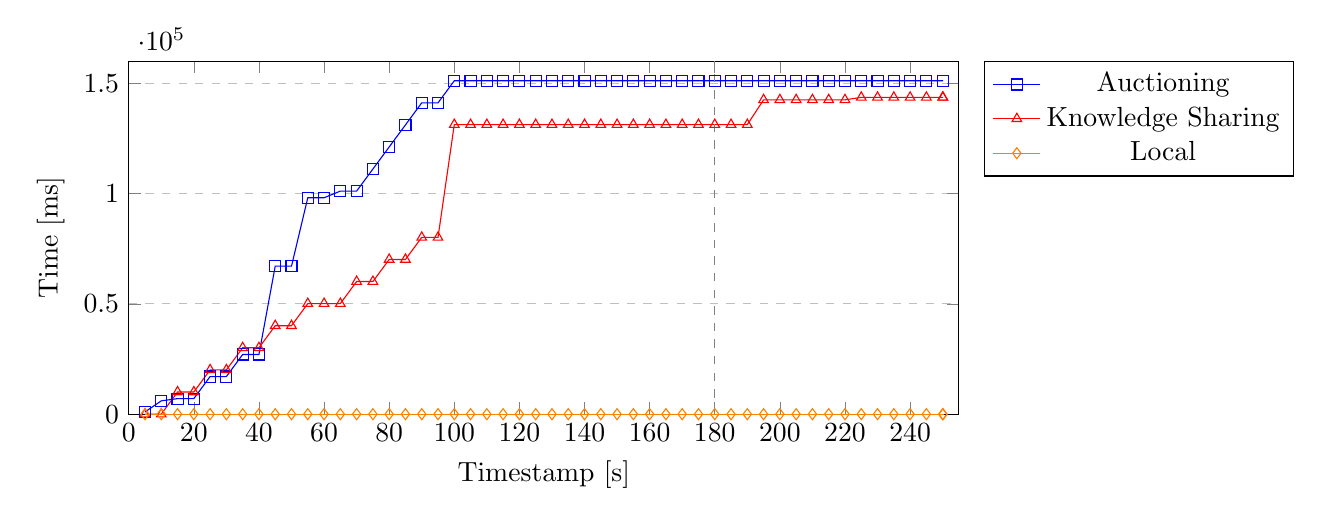
\begin{tikzpicture}
\begin{axis}[
    xlabel={Timestamp [s]},
    ylabel={Time [ms]},
    xmin=0, xmax=255000,
    ymin=0, ymax=160016,
    legend pos=outer north east,
    ymajorgrids=true,
    grid style=dashed,
    width=\textwidth,
    height=0.5\textwidth,
    scaled x ticks=base 10:-3,
    xtick scale label code/.code={}
]

	\addplot[color=blue,mark=square] coordinates {
        (5000,1002)(10000,6043)(15000,7052)(20000,7052)(25000,17062)(30000,17062)(35000,27073)(40000,27073)(45000,67114)(50000,67114)(55000,98143)(60000,98143)(65000,101166)(70000,101166)(75000,111175)(80000,121177)(85000,131184)(90000,141191)(95000,141191)(100000,151201)(105000,151201)(110000,151201)(115000,151201)(120000,151201)(125000,151201)(130000,151201)(135000,151201)(140000,151201)(145000,151201)(150000,151201)(155000,151201)(160000,151201)(165000,151201)(170000,151201)(175000,151201)(180000,151201)(185000,151201)(190000,151201)(195000,151201)(200000,151201)(205000,151201)(210000,151201)(215000,151201)(220000,151201)(225000,151201)(230000,151201)(235000,151201)(240000,151201)(245000,151201)(250000,151201)(250139,151201)
    };
    \addlegendentry{Auctioning}
	\addplot[color=red,mark=triangle] coordinates {
        (5000,0)(10000,0)(15000,10047)(20000,10047)(25000,20080)(30000,20080)(35000,30102)(40000,30102)(45000,40126)(50000,40126)(55000,50144)(60000,50144)(65000,50144)(70000,60152)(75000,60152)(80000,70161)(85000,70161)(90000,80163)(95000,80163)(100000,131322)(105000,131322)(110000,131322)(115000,131322)(120000,131322)(125000,131322)(130000,131322)(135000,131322)(140000,131322)(145000,131322)(150000,131322)(155000,131322)(160000,131322)(165000,131322)(170000,131322)(175000,131322)(180000,131322)(185000,131322)(190000,131322)(195000,142557)(200000,142557)(205000,142557)(210000,142557)(215000,142557)(220000,142557)(225000,143673)(230000,143673)(235000,143673)(240000,143673)(245000,143673)(250000,143673)(250111,143673)
    };
    \addlegendentry{Knowledge Sharing}
	\addplot[color=orange,mark=diamond] coordinates {
        (5000,0)(10000,0)(15000,0)(20000,0)(25000,0)(30000,0)(35000,0)(40000,0)(45000,0)(50000,0)(55000,0)(60000,0)(65000,0)(70000,0)(75000,0)(80000,0)(85000,0)(90000,0)(95000,0)(100000,0)(105000,0)(110000,0)(115000,0)(120000,0)(125000,0)(130000,0)(135000,0)(140000,0)(145000,0)(150000,0)(155000,0)(160000,0)(165000,0)(170000,0)(175000,0)(180000,0)(185000,0)(190000,0)(195000,0)(200000,0)(205000,0)(210000,0)(215000,0)(220000,0)(225000,0)(230000,0)(235000,0)(240000,0)(245000,0)(250000,0)(250115,0)
    };
    \addlegendentry{Local}

	\addplot[color=gray, dashed,] coordinates {(180000,0) (180000,160016)};


\end{axis}
\end{tikzpicture}
    \caption{Graph showing the sum of time spent adapting by agents in the risk introduction scenario.}
    \label{fig:adapting-time-risk-introduction}
\end{figure}

Figure \ref{fig:adapting-time-risk-introduction} shows that the knowledge-sharing agent is still spending more time adapting compared to the auctioning agent. Compared to Figure \ref{fig:adapting-time-no-change} we see that the agents are all spending roughly the same amount of time adapting, until the $120$ second mark. After this time a bump is observable in the graph.

\subsection{Scenario 3: Growing Infrastructure}
\textit{This scenario introduces a new infrastructure node every $30$ seconds. The purpose of this scenario is to see how the system behaves when the infrastructure is growing.}

\begin{figure}[H]
    \centering
    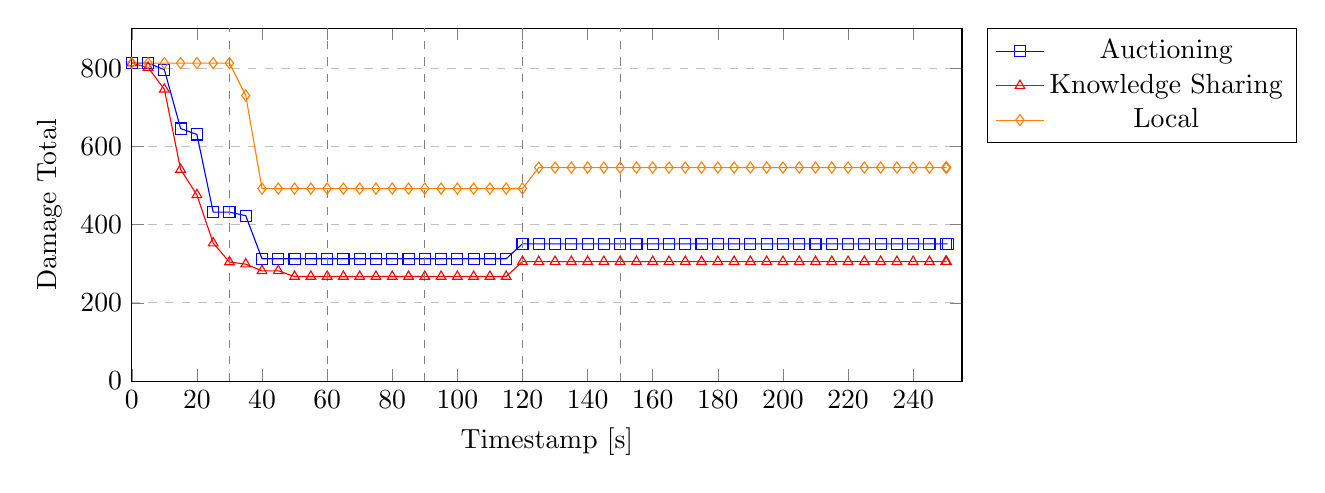
\begin{tikzpicture}
\begin{axis}[
    xlabel={Timestamp [s]},
    ylabel={Damage Total},
    xmin=0, xmax=255000,
    ymin=0, ymax=902,
    legend pos=outer north east,
    ymajorgrids=true,
    grid style=dashed,
    width=\textwidth,
    height=0.5\textwidth,
    scaled x ticks=base 10:-3,
    xtick scale label code/.code={}
]

	\addplot[color=blue,mark=square] coordinates {
        (0,812.71)(5000,812.71)(10000,796.17)(15000,645.46)(20000,630.54)(25000,431.97)(30000,431.97)(35000,422.77)(40000,312.76)(45000,312.76)(50000,312.76)(55000,312.76)(60000,312.76)(65000,312.76)(70000,312.76)(75000,312.76)(80000,312.76)(85000,312.76)(90000,312.76)(95000,312.76)(100000,312.76)(105000,312.76)(110000,312.76)(115000,312.76)(120000,350.90)(125000,350.90)(130000,350.90)(135000,350.90)(140000,350.90)(145000,350.90)(150000,350.90)(155000,350.90)(160000,350.90)(165000,350.90)(170000,350.90)(175000,350.90)(180000,350.90)(185000,350.90)(190000,350.90)(195000,350.90)(200000,350.90)(205000,350.90)(210000,350.90)(215000,350.90)(220000,350.90)(225000,350.90)(230000,350.90)(235000,350.90)(240000,350.90)(245000,350.90)(250000,350.90)(250569,350.90)
    };
    \addlegendentry{Auctioning}
	\addplot[color=red,mark=triangle] coordinates {
        (0,812.71)(5000,801.69)(10000,745.99)(15000,541.01)(20000,476.06)(25000,352.72)(30000,304.33)(35000,298.99)(40000,281.89)(45000,281.89)(50000,267.31)(55000,267.31)(60000,267.31)(65000,267.31)(70000,267.31)(75000,267.31)(80000,267.31)(85000,267.31)(90000,267.31)(95000,267.31)(100000,267.31)(105000,267.31)(110000,267.31)(115000,267.31)(120000,305.45)(125000,305.45)(130000,305.45)(135000,305.45)(140000,305.45)(145000,305.45)(150000,305.45)(155000,305.45)(160000,305.45)(165000,305.45)(170000,305.45)(175000,305.45)(180000,305.45)(185000,305.45)(190000,305.45)(195000,305.45)(200000,305.45)(205000,305.45)(210000,305.45)(215000,305.45)(220000,305.45)(225000,305.45)(230000,305.45)(235000,305.45)(240000,305.45)(245000,305.45)(250000,305.45)(250242,305.45)
    };
    \addlegendentry{Knowledge Sharing}
	\addplot[color=orange,mark=diamond] coordinates {
        (0,812.71)(5000,812.71)(10000,812.71)(15000,812.71)(20000,812.71)(25000,812.71)(30000,812.71)(35000,729.98)(40000,492.04)(45000,492.04)(50000,492.04)(55000,492.04)(60000,492.04)(65000,492.04)(70000,492.04)(75000,492.04)(80000,492.04)(85000,492.04)(90000,492.04)(95000,492.04)(100000,492.04)(105000,492.04)(110000,492.04)(115000,492.04)(120000,492.04)(125000,545.78)(130000,545.78)(135000,545.78)(140000,545.78)(145000,545.78)(150000,545.78)(155000,545.78)(160000,545.78)(165000,545.78)(170000,545.78)(175000,545.78)(180000,545.78)(185000,545.78)(190000,545.78)(195000,545.78)(200000,545.78)(205000,545.78)(210000,545.78)(215000,545.78)(220000,545.78)(225000,545.78)(230000,545.78)(235000,545.78)(240000,545.78)(245000,545.78)(250000,545.78)(250282,545.78)
    };
    \addlegendentry{Local}

	\addplot[color=gray, dashed,] coordinates {(30000,0) (30000,902)};
	\addplot[color=gray, dashed,] coordinates {(60000,0) (60000,902)};
	\addplot[color=gray, dashed,] coordinates {(90000,0) (90000,902)};
	\addplot[color=gray, dashed,] coordinates {(120000,0) (120000,902)};
	\addplot[color=gray, dashed,] coordinates {(150000,0) (150000,902)};


\end{axis}
\end{tikzpicture}
    \caption{This graph shows the overall damage of the system in the growing scenario. The damage is shown for each of the three strategies. The vertical lines indicate the time at which a node is introduced.}
    \label{fig:overall-damage-growing}
\end{figure}

From Figure \ref{fig:overall-damage-growing} we see that the auctioning and knowledge-sharing agents are able to keep the damage at a stable level, even though the infrastructure is growing. Only at the end do we see that the agents cannot cope with the increasing damage and does the damage increase. The auctioning agent is keeping the overall damage at the lowest point. This is a good result, as the infrastructure is growing, and the agents are able to keep the damage at a low level. 
As mentioned before, the damage is calculated at a $5000$ms interval. This means that the damage could be higher than the graph shows, as adaptations could be applied within the timeframe. This is the case for the auctioning agent and knowledge-sharing agent, which is observed in the log-files. However, the local-agent does not apply any adaptations during this time, this is visible in the diverging lines at the end of the graph.
 
\begin{figure}[H]
    \centering
    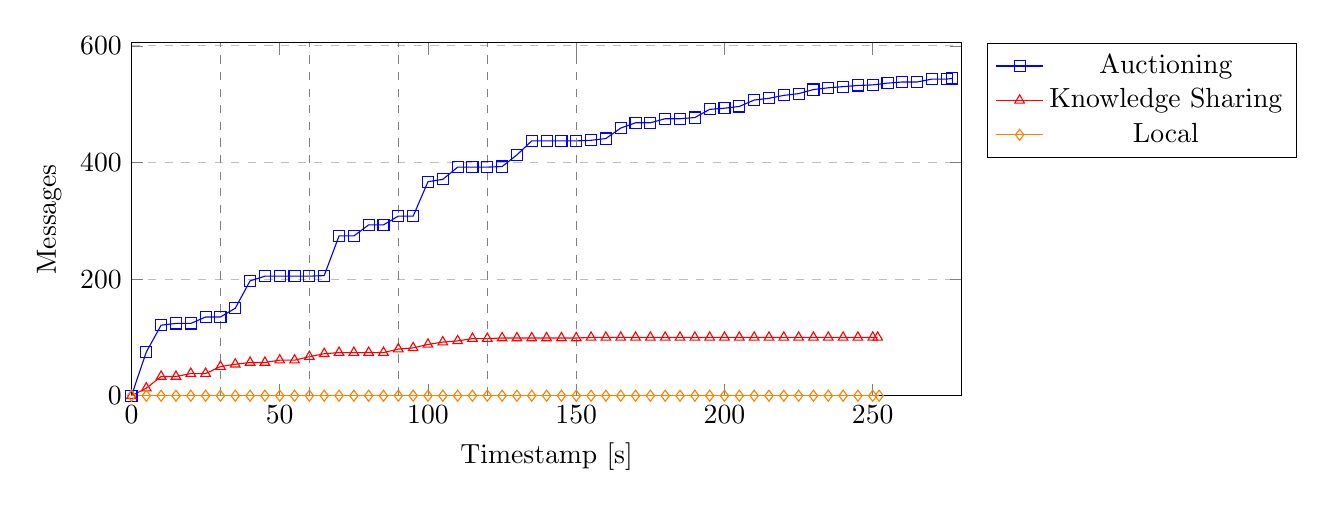
\begin{tikzpicture}
\begin{axis}[
    xlabel={Timestamp [s]},
    ylabel={Messages},
    xmin=0, xmax=280000,
    ymin=0, ymax=605,
    legend pos=outer north east,
    ymajorgrids=true,
    grid style=dashed,
    width=\textwidth,
    height=0.5\textwidth,
    scaled x ticks=base 10:-3,
    xtick scale label code/.code={}
]

	\addplot[color=blue,mark=square] coordinates {
        (0,0)(5000,75)(10000,121)(15000,124)(20000,124)(25000,135)(30000,135)(35000,150)(40000,197)(45000,205)(50000,205)(55000,205)(60000,205)(65000,206)(70000,274)(75000,274)(80000,293)(85000,293)(90000,308)(95000,308)(100000,367)(105000,371)(110000,392)(115000,392)(120000,392)(125000,393)(130000,413)(135000,437)(140000,437)(145000,437)(150000,437)(155000,438)(160000,441)(165000,459)(170000,468)(175000,468)(180000,475)(185000,475)(190000,477)(195000,491)(200000,493)(205000,496)(210000,507)(215000,510)(220000,515)(225000,518)(230000,525)(235000,528)(240000,530)(245000,532)(250000,533)(255000,536)(260000,538)(265000,538)(270000,543)(275000,543)(276704,544)
    };
    \addlegendentry{Auctioning}
	\addplot[color=red,mark=triangle] coordinates {
        (0,0)(5000,13)(10000,33)(15000,33)(20000,38)(25000,38)(30000,50)(35000,54)(40000,57)(45000,57)(50000,61)(55000,61)(60000,67)(65000,72)(70000,74)(75000,74)(80000,74)(85000,74)(90000,80)(95000,82)(100000,88)(105000,92)(110000,94)(115000,98)(120000,98)(125000,99)(130000,99)(135000,99)(140000,99)(145000,99)(150000,99)(155000,100)(160000,100)(165000,100)(170000,100)(175000,100)(180000,100)(185000,100)(190000,100)(195000,100)(200000,100)(205000,100)(210000,100)(215000,100)(220000,100)(225000,100)(230000,100)(235000,100)(240000,100)(245000,100)(250000,100)(251678,100)
    };
    \addlegendentry{Knowledge Sharing}
	\addplot[color=orange,mark=diamond] coordinates {
        (0,0)(5000,0)(10000,0)(15000,0)(20000,0)(25000,0)(30000,0)(35000,0)(40000,0)(45000,0)(50000,0)(55000,0)(60000,0)(65000,0)(70000,0)(75000,0)(80000,0)(85000,0)(90000,0)(95000,0)(100000,0)(105000,0)(110000,0)(115000,0)(120000,0)(125000,0)(130000,0)(135000,0)(140000,0)(145000,0)(150000,0)(155000,0)(160000,0)(165000,0)(170000,0)(175000,0)(180000,0)(185000,0)(190000,0)(195000,0)(200000,0)(205000,0)(210000,0)(215000,0)(220000,0)(225000,0)(230000,0)(235000,0)(240000,0)(245000,0)(250000,0)(252143,0)
    };
    \addlegendentry{Local}

	\addplot[color=gray, dashed,] coordinates {(30000,0) (30000,605)};
	\addplot[color=gray, dashed,] coordinates {(60000,0) (60000,605)};
	\addplot[color=gray, dashed,] coordinates {(90000,0) (90000,605)};
	\addplot[color=gray, dashed,] coordinates {(120000,0) (120000,605)};
	\addplot[color=gray, dashed,] coordinates {(150000,0) (150000,605)};


\end{axis}
\end{tikzpicture}
    \caption{Graph showing the total amount of messages sent between agents in the growing infrastructure scenario.}
    \label{fig:messages-growing}
\end{figure}

Figure \ref{fig:messages-growing} shows that the auctioning agent sends the most messages, followed by the knowledge-sharing agent. The local-agent sends no messages. We see that both the auctioning and knowledge-sharing agents send a few messages around every time a new node is introduced. This is to be expected as the agents detect a change in their properties, and start sharing this information with other agents.

\begin{figure}[H]
    \centering
    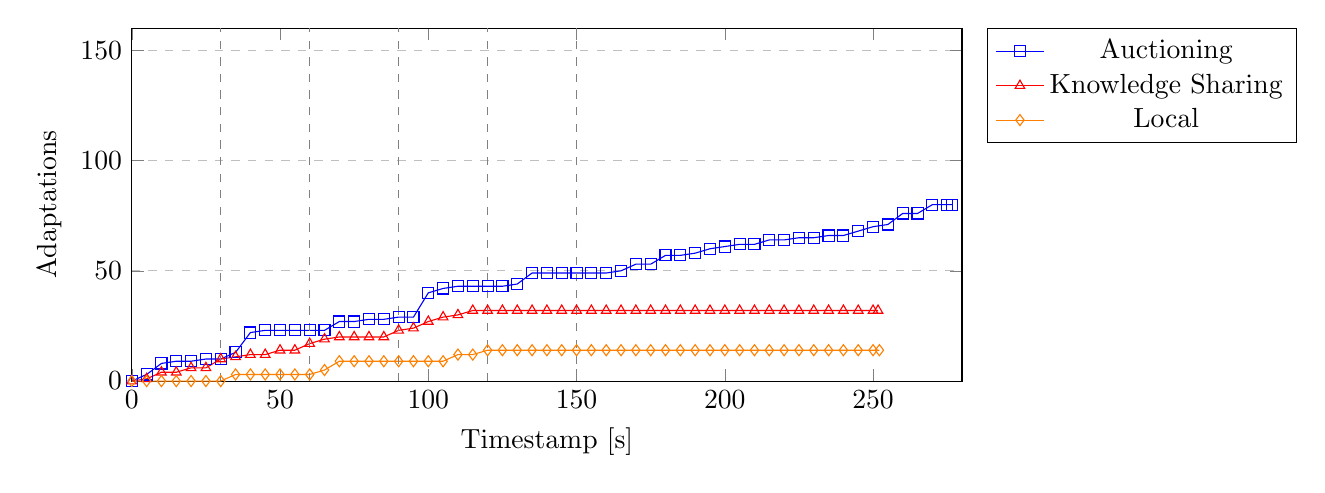
\begin{tikzpicture}
\begin{axis}[
    xlabel={Timestamp [s]},
    ylabel={Adaptations},
    xmin=0, xmax=280000,
    ymin=0, ymax=160,
    legend pos=outer north east,
    ymajorgrids=true,
    grid style=dashed,
    width=\textwidth,
    height=0.5\textwidth,
    scaled x ticks=base 10:-3,
    xtick scale label code/.code={}
]

	\addplot[color=blue,mark=square] coordinates {
        (0,0)(5000,3)(10000,8)(15000,9)(20000,9)(25000,10)(30000,10)(35000,13)(40000,22)(45000,23)(50000,23)(55000,23)(60000,23)(65000,23)(70000,27)(75000,27)(80000,28)(85000,28)(90000,29)(95000,29)(100000,40)(105000,42)(110000,43)(115000,43)(120000,43)(125000,43)(130000,44)(135000,49)(140000,49)(145000,49)(150000,49)(155000,49)(160000,49)(165000,50)(170000,53)(175000,53)(180000,57)(185000,57)(190000,58)(195000,60)(200000,61)(205000,62)(210000,62)(215000,64)(220000,64)(225000,65)(230000,65)(235000,66)(240000,66)(245000,68)(250000,70)(255000,71)(260000,76)(265000,76)(270000,80)(275000,80)(276704,80)
    };
    \addlegendentry{Auctioning}
	\addplot[color=red,mark=triangle] coordinates {
        (0,0)(5000,1)(10000,4)(15000,4)(20000,6)(25000,6)(30000,10)(35000,11)(40000,12)(45000,12)(50000,14)(55000,14)(60000,17)(65000,19)(70000,20)(75000,20)(80000,20)(85000,20)(90000,23)(95000,24)(100000,27)(105000,29)(110000,30)(115000,32)(120000,32)(125000,32)(130000,32)(135000,32)(140000,32)(145000,32)(150000,32)(155000,32)(160000,32)(165000,32)(170000,32)(175000,32)(180000,32)(185000,32)(190000,32)(195000,32)(200000,32)(205000,32)(210000,32)(215000,32)(220000,32)(225000,32)(230000,32)(235000,32)(240000,32)(245000,32)(250000,32)(251678,32)
    };
    \addlegendentry{Knowledge Sharing}
	\addplot[color=orange,mark=diamond] coordinates {
        (0,0)(5000,0)(10000,0)(15000,0)(20000,0)(25000,0)(30000,0)(35000,3)(40000,3)(45000,3)(50000,3)(55000,3)(60000,3)(65000,5)(70000,9)(75000,9)(80000,9)(85000,9)(90000,9)(95000,9)(100000,9)(105000,9)(110000,12)(115000,12)(120000,14)(125000,14)(130000,14)(135000,14)(140000,14)(145000,14)(150000,14)(155000,14)(160000,14)(165000,14)(170000,14)(175000,14)(180000,14)(185000,14)(190000,14)(195000,14)(200000,14)(205000,14)(210000,14)(215000,14)(220000,14)(225000,14)(230000,14)(235000,14)(240000,14)(245000,14)(250000,14)(252143,14)
    };
    \addlegendentry{Local}

	\addplot[color=gray, dashed,] coordinates {(30000,0) (30000,160)};
	\addplot[color=gray, dashed,] coordinates {(60000,0) (60000,160)};
	\addplot[color=gray, dashed,] coordinates {(90000,0) (90000,160)};
	\addplot[color=gray, dashed,] coordinates {(120000,0) (120000,160)};
	\addplot[color=gray, dashed,] coordinates {(150000,0) (150000,160)};


\end{axis}
\end{tikzpicture}
    \caption{Graph showing the total amount of adaptations applied by agents in the growing scenario.}
    \label{fig:proposals-growing}
\end{figure}

As for the adaptations in this experiment, we also see a gradual increase in proposals over time. The local agent is unable to cope with the changes to the infrastructure, and is unable to apply any adaptations. We see that the auctioning agent is slowly applying adaptations, where the knowledge-sharing agent applies them like in quick succession. This is to be expected as the auctioning agent has to negotiate the adaptations, which takes time.

\begin{figure}[H]
    \centering
        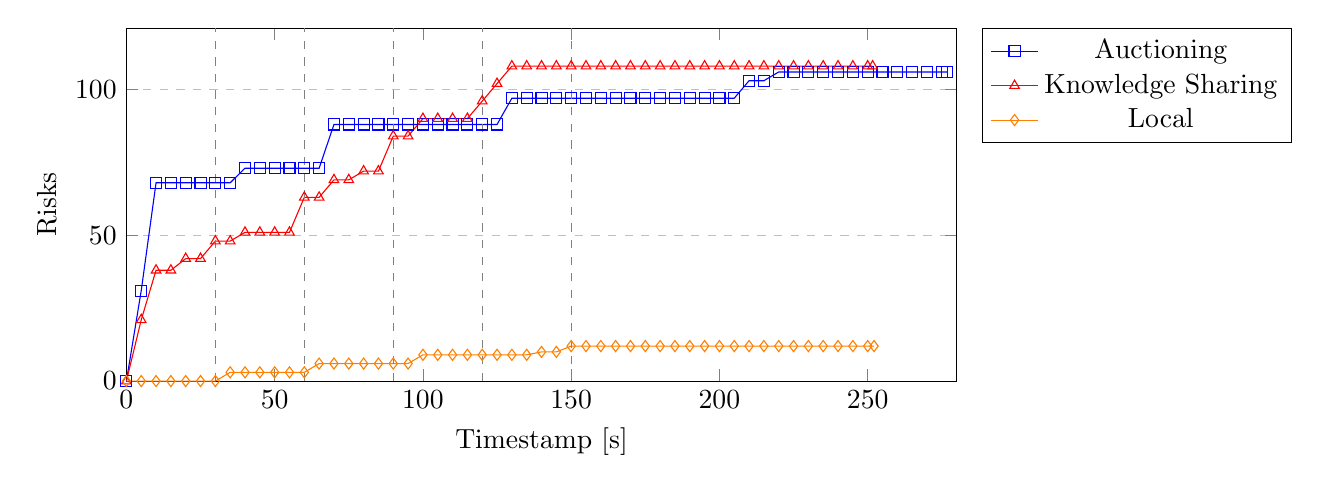
\begin{tikzpicture}
\begin{axis}[
    xlabel={Timestamp [s]},
    ylabel={Risks},
    xmin=0, xmax=280000,
    ymin=0, ymax=121,
    legend pos=outer north east,
    ymajorgrids=true,
    grid style=dashed,
    width=\textwidth,
    height=0.5\textwidth,
    scaled x ticks=base 10:-3,
    xtick scale label code/.code={}
]

	\addplot[color=blue,mark=square] coordinates {
        (0,0)(5000,31)(10000,68)(15000,68)(20000,68)(25000,68)(30000,68)(35000,68)(40000,73)(45000,73)(50000,73)(55000,73)(60000,73)(65000,73)(70000,88)(75000,88)(80000,88)(85000,88)(90000,88)(95000,88)(100000,88)(105000,88)(110000,88)(115000,88)(120000,88)(125000,88)(130000,97)(135000,97)(140000,97)(145000,97)(150000,97)(155000,97)(160000,97)(165000,97)(170000,97)(175000,97)(180000,97)(185000,97)(190000,97)(195000,97)(200000,97)(205000,97)(210000,103)(215000,103)(220000,106)(225000,106)(230000,106)(235000,106)(240000,106)(245000,106)(250000,106)(255000,106)(260000,106)(265000,106)(270000,106)(275000,106)(276704,106)
    };
    \addlegendentry{Auctioning}
	\addplot[color=red,mark=triangle] coordinates {
        (0,0)(5000,21)(10000,38)(15000,38)(20000,42)(25000,42)(30000,48)(35000,48)(40000,51)(45000,51)(50000,51)(55000,51)(60000,63)(65000,63)(70000,69)(75000,69)(80000,72)(85000,72)(90000,84)(95000,84)(100000,90)(105000,90)(110000,90)(115000,90)(120000,96)(125000,102)(130000,108)(135000,108)(140000,108)(145000,108)(150000,108)(155000,108)(160000,108)(165000,108)(170000,108)(175000,108)(180000,108)(185000,108)(190000,108)(195000,108)(200000,108)(205000,108)(210000,108)(215000,108)(220000,108)(225000,108)(230000,108)(235000,108)(240000,108)(245000,108)(250000,108)(251678,108)
    };
    \addlegendentry{Knowledge Sharing}
	\addplot[color=orange,mark=diamond] coordinates {
        (0,0)(5000,0)(10000,0)(15000,0)(20000,0)(25000,0)(30000,0)(35000,3)(40000,3)(45000,3)(50000,3)(55000,3)(60000,3)(65000,6)(70000,6)(75000,6)(80000,6)(85000,6)(90000,6)(95000,6)(100000,9)(105000,9)(110000,9)(115000,9)(120000,9)(125000,9)(130000,9)(135000,9)(140000,10)(145000,10)(150000,12)(155000,12)(160000,12)(165000,12)(170000,12)(175000,12)(180000,12)(185000,12)(190000,12)(195000,12)(200000,12)(205000,12)(210000,12)(215000,12)(220000,12)(225000,12)(230000,12)(235000,12)(240000,12)(245000,12)(250000,12)(252143,12)
    };
    \addlegendentry{Local}

	\addplot[color=gray, dashed,] coordinates {(30000,0) (30000,121)};
	\addplot[color=gray, dashed,] coordinates {(60000,0) (60000,121)};
	\addplot[color=gray, dashed,] coordinates {(90000,0) (90000,121)};
	\addplot[color=gray, dashed,] coordinates {(120000,0) (120000,121)};
	\addplot[color=gray, dashed,] coordinates {(150000,0) (150000,121)};


\end{axis}
\end{tikzpicture}
    \caption{Graph showing the number of unique risks detected by agents in the growing scenario.}
    \label{fig:risk-count-growing}
\end{figure}

Figure \ref{fig:risk-count-growing} show that the knowledge-sharing agent finds the most unique risks, followed by the auctioning agent. The auctioning agent finds only $50\%$ of the risks detected by the knowledge-sharing agent. The local-agent finds the least amount of risks, at only $10\%$ of the risks found by the knowledge-sharing agent. As mentioned in Section \ref{ssec:scenario-2-results}, this is likely due to the fact that in the knowledge-sharing setup agents apply multiple adaptations in parallel. 

\begin{figure}[H]
    \centering
        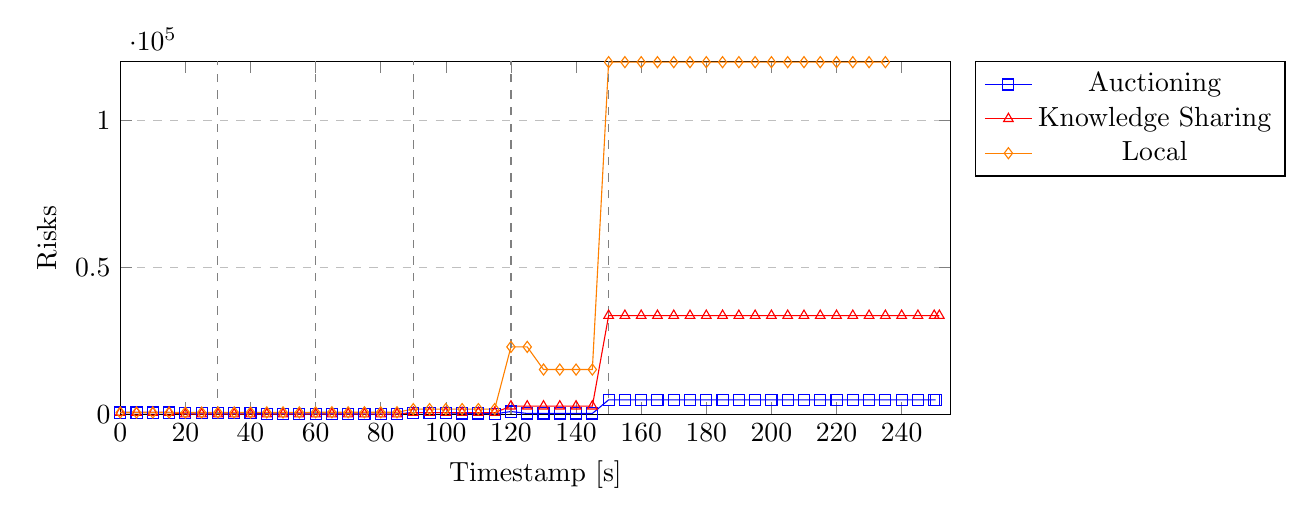
\begin{tikzpicture}
\begin{axis}[
    xlabel={Timestamp [s]},
    ylabel={Risks},
    xmin=0, xmax=255000,
    ymin=0, ymax=120012,
    legend pos=outer north east,
    ymajorgrids=true,
    grid style=dashed,
    width=\textwidth,
    height=0.5\textwidth,
    scaled x ticks=base 10:-3,
    xtick scale label code/.code={}
]

	\addplot[color=blue,mark=square] coordinates {
        (0,563)(5000,563)(10000,563)(15000,563)(20000,360)(25000,360)(30000,399)(35000,399)(40000,399)(45000,100)(50000,100)(55000,60)(60000,80)(65000,80)(70000,80)(75000,40)(80000,40)(85000,40)(90000,520)(95000,520)(100000,520)(105000,240)(110000,240)(115000,100)(120000,900)(125000,240)(130000,240)(135000,240)(140000,240)(145000,240)(150000,4880)(155000,4880)(160000,4880)(165000,4880)(170000,4880)(175000,4880)(180000,4880)(185000,4880)(190000,4880)(195000,4880)(200000,4880)(205000,4880)(210000,4880)(215000,4880)(220000,4880)(225000,4880)(230000,4880)(235000,4880)(240000,4880)(245000,4880)(250000,4880)(250452,4880)
    };
    \addlegendentry{Auctioning}
	\addplot[color=red,mark=triangle] coordinates {
        (0,563)(5000,563)(10000,563)(15000,563)(20000,10)(25000,10)(30000,40)(35000,20)(40000,20)(45000,20)(50000,20)(55000,20)(60000,40)(65000,40)(70000,40)(75000,40)(80000,40)(85000,40)(90000,520)(95000,520)(100000,520)(105000,520)(110000,520)(115000,520)(120000,2720)(125000,2720)(130000,2720)(135000,2720)(140000,2720)(145000,2720)(150000,33540)(155000,33540)(160000,33540)(165000,33540)(170000,33540)(175000,33540)(180000,33540)(185000,33540)(190000,33540)(195000,33540)(200000,33540)(205000,33540)(210000,33540)(215000,33540)(220000,33540)(225000,33540)(230000,33540)(235000,33540)(240000,33540)(245000,33540)(250000,33540)(251574,33540)
    };
    \addlegendentry{Knowledge Sharing}
	\addplot[color=orange,mark=diamond] coordinates {
        (0,563)(5000,563)(10000,563)(15000,563)(20000,563)(25000,563)(30000,608)(35000,608)(40000,608)(45000,608)(50000,608)(55000,608)(60000,653)(65000,653)(70000,653)(75000,653)(80000,653)(85000,653)(90000,1733)(95000,1733)(100000,1733)(105000,1733)(110000,1733)(115000,1733)(120000,22883)(125000,22883)(130000,15180)(135000,15180)(140000,15180)(145000,15180)(150000,119730)(155000,119730)(160000,119730)(165000,119730)(170000,119730)(175000,119730)(180000,119730)(185000,119730)(190000,119730)(195000,119730)(200000,119730)(205000,119730)(210000,119730)(215000,119730)(220000,119730)(225000,119730)(230000,119730)(235000,119730)
    };
    \addlegendentry{Local}

	\addplot[color=gray, dashed,] coordinates {(30000,0) (30000,120012)};
	\addplot[color=gray, dashed,] coordinates {(60000,0) (60000,120012)};
	\addplot[color=gray, dashed,] coordinates {(90000,0) (90000,120012)};
	\addplot[color=gray, dashed,] coordinates {(120000,0) (120000,120012)};
	\addplot[color=gray, dashed,] coordinates {(150000,0) (150000,120012)};


\end{axis}
\end{tikzpicture}
    \caption{Graph showing the number of remaining risks in the infrastructure in the growing scenario.}
    \label{fig:risk-remaining-growing}
\end{figure}

\add{write}

\begin{figure}[H]
    \hspace*{-1cm}
    \centering
        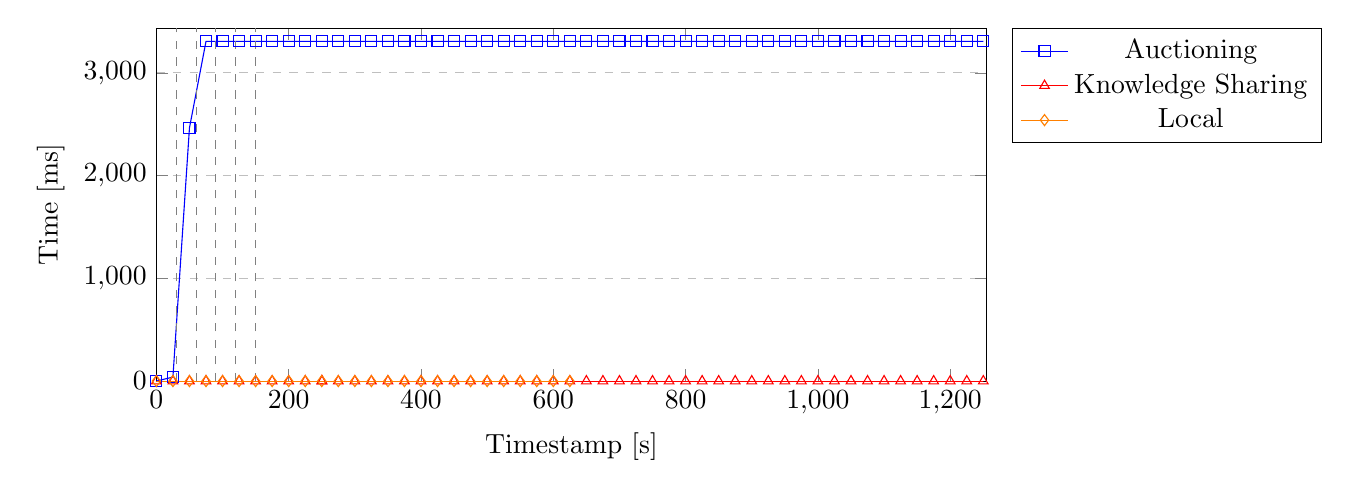
\begin{tikzpicture}
\begin{axis}[
    xlabel={Timestamp [s]},
    ylabel={Time [ms]},
    xmin=0, xmax=1255000,
    ymin=0, ymax=3434,
    legend pos=outer north east,
    ymajorgrids=true,
    grid style=dashed,
    width=\textwidth,
    height=0.5\textwidth,
    scaled x ticks=base 10:-3,
    xtick scale label code/.code={}
]

	\addplot[color=blue,mark=square] coordinates {
        (0,0)(25000,39)(50000,2464)(75000,3306)(100000,3306)(125000,3306)(150000,3306)(175000,3306)(200000,3306)(225000,3306)(250000,3306)(275000,3306)(300000,3306)(325000,3306)(350000,3306)(375000,3306)(400000,3306)(425000,3306)(450000,3306)(475000,3306)(500000,3306)(525000,3306)(550000,3306)(575000,3306)(600000,3306)(625000,3306)(650000,3306)(675000,3306)(700000,3306)(725000,3306)(750000,3306)(775000,3306)(800000,3306)(825000,3306)(850000,3306)(875000,3306)(900000,3306)(925000,3306)(950000,3306)(975000,3306)(1000000,3306)(1025000,3306)(1050000,3306)(1075000,3306)(1100000,3306)(1125000,3306)(1150000,3306)(1175000,3306)(1200000,3306)(1225000,3306)(1250000,3306)(250447,3306)
    };
    \addlegendentry{Auctioning}
	\addplot[color=red,mark=triangle] coordinates {
        (0,0)(25000,0)(50000,0)(75000,0)(100000,0)(125000,0)(150000,0)(175000,0)(200000,0)(225000,0)(250000,0)(275000,0)(300000,0)(325000,0)(350000,0)(375000,0)(400000,0)(425000,0)(450000,0)(475000,0)(500000,0)(525000,0)(550000,0)(575000,0)(600000,0)(625000,0)(650000,0)(675000,0)(700000,0)(725000,0)(750000,0)(775000,0)(800000,0)(825000,0)(850000,0)(875000,0)(900000,0)(925000,0)(950000,0)(975000,0)(1000000,0)(1025000,0)(1050000,0)(1075000,0)(1100000,0)(1125000,0)(1150000,0)(1175000,0)(1200000,0)(1225000,0)(1250000,0)(250418,0)
    };
    \addlegendentry{Knowledge Sharing}
	\addplot[color=orange,mark=diamond] coordinates {
        (0,0)(25000,0)(50000,0)(75000,0)(100000,0)(125000,0)(150000,0)(175000,0)(200000,0)(225000,0)(250000,0)(275000,0)(300000,0)(325000,0)(350000,0)(375000,0)(400000,0)(425000,0)(450000,0)(475000,0)(500000,0)(525000,0)(550000,0)(575000,0)(600000,0)(625000,0)
    };
    \addlegendentry{Local}

	\addplot[color=gray, dashed,] coordinates {(30000,0) (30000,3434)};
	\addplot[color=gray, dashed,] coordinates {(60000,0) (60000,3434)};
	\addplot[color=gray, dashed,] coordinates {(90000,0) (90000,3434)};
	\addplot[color=gray, dashed,] coordinates {(120000,0) (120000,3434)};
	\addplot[color=gray, dashed,] coordinates {(150000,0) (150000,3434)};


\end{axis}
\end{tikzpicture}
    \caption{Graph showing the sum of time spent auctioning by agents in the growing scenario.}
    \label{fig:auctioning-time-growing}
\end{figure}

Figure \ref{fig:auctioning-time-growing} shows an ever growing amount of time spent auctioning. This is in line with the expectations as the agents finds a risk, and then starts an auction. These auctions in the end lead to no proposals/adaptations being applied, as the agents are unable to find a better adaptation. This is visible in the graph as the time spent auctioning increases, but the amount of adaptations from Figure \ref{fig:proposals-growing} stays the same.

\begin{figure}[H]
    \hspace*{-1cm}
    \centering
        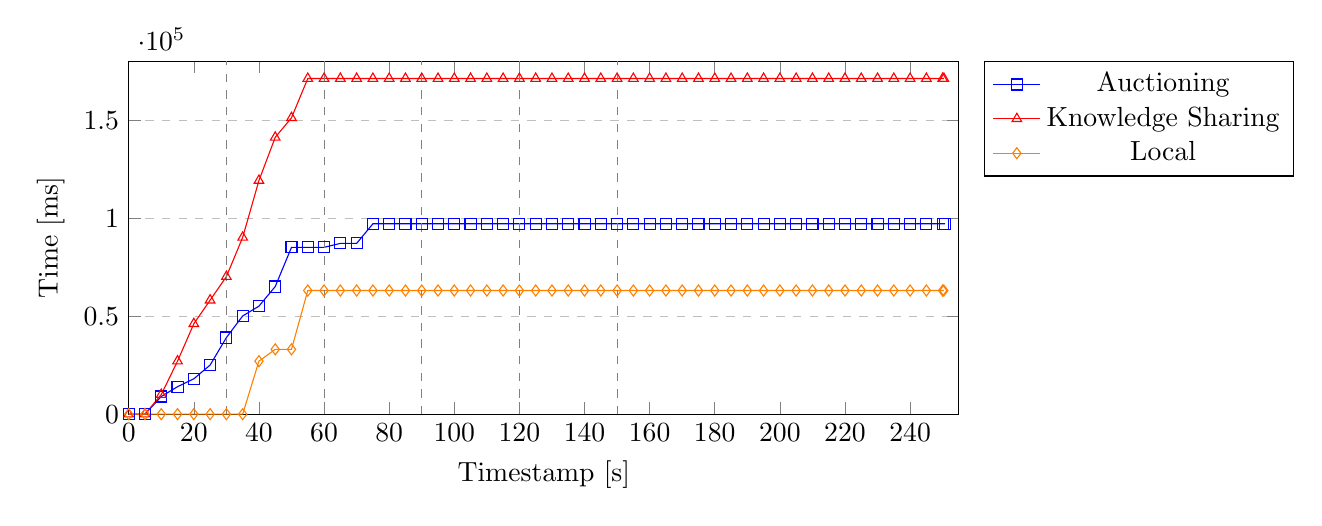
\begin{tikzpicture}
\begin{axis}[
    xlabel={Timestamp [s]},
    ylabel={Time [ms]},
    xmin=0, xmax=255000,
    ymin=0, ymax=180018,
    legend pos=outer north east,
    ymajorgrids=true,
    grid style=dashed,
    width=\textwidth,
    height=0.5\textwidth,
    scaled x ticks=base 10:-3,
    xtick scale label code/.code={}
]

	\addplot[color=blue,mark=square] coordinates {
        (0,0)(5000,0)(10000,9022)(15000,14028)(20000,18038)(25000,25054)(30000,39076)(35000,50106)(40000,55112)(45000,65114)(50000,85122)(55000,85122)(60000,85122)(65000,87124)(70000,87124)(75000,97131)(80000,97131)(85000,97131)(90000,97131)(95000,97131)(100000,97131)(105000,97131)(110000,97131)(115000,97131)(120000,97131)(125000,97131)(130000,97131)(135000,97131)(140000,97131)(145000,97131)(150000,97131)(155000,97131)(160000,97131)(165000,97131)(170000,97131)(175000,97131)(180000,97131)(185000,97131)(190000,97131)(195000,97131)(200000,97131)(205000,97131)(210000,97131)(215000,97131)(220000,97131)(225000,97131)(230000,97131)(235000,97131)(240000,97131)(245000,97131)(250000,97131)(250721,97131)
    };
    \addlegendentry{Auctioning}
	\addplot[color=red,mark=triangle] coordinates {
        (0,0)(5000,0)(10000,10020)(15000,27063)(20000,46118)(25000,58158)(30000,70170)(35000,90181)(40000,119203)(45000,141218)(50000,151223)(55000,171237)(60000,171237)(65000,171237)(70000,171237)(75000,171237)(80000,171237)(85000,171237)(90000,171237)(95000,171237)(100000,171237)(105000,171237)(110000,171237)(115000,171237)(120000,171237)(125000,171237)(130000,171237)(135000,171237)(140000,171237)(145000,171237)(150000,171237)(155000,171237)(160000,171237)(165000,171237)(170000,171237)(175000,171237)(180000,171237)(185000,171237)(190000,171237)(195000,171237)(200000,171237)(205000,171237)(210000,171237)(215000,171237)(220000,171237)(225000,171237)(230000,171237)(235000,171237)(240000,171237)(245000,171237)(250000,171237)(250388,171237)
    };
    \addlegendentry{Knowledge Sharing}
	\addplot[color=orange,mark=diamond] coordinates {
        (0,0)(5000,0)(10000,0)(15000,0)(20000,0)(25000,0)(30000,0)(35000,0)(40000,27063)(45000,33082)(50000,33082)(55000,63089)(60000,63089)(65000,63089)(70000,63089)(75000,63089)(80000,63089)(85000,63089)(90000,63089)(95000,63089)(100000,63089)(105000,63089)(110000,63089)(115000,63089)(120000,63089)(125000,63089)(130000,63089)(135000,63089)(140000,63089)(145000,63089)(150000,63089)(155000,63089)(160000,63089)(165000,63089)(170000,63089)(175000,63089)(180000,63089)(185000,63089)(190000,63089)(195000,63089)(200000,63089)(205000,63089)(210000,63089)(215000,63089)(220000,63089)(225000,63089)(230000,63089)(235000,63089)(240000,63089)(245000,63089)(250000,63089)(250358,63089)
    };
    \addlegendentry{Local}

	\addplot[color=gray, dashed,] coordinates {(30000,0) (30000,180018)};
	\addplot[color=gray, dashed,] coordinates {(60000,0) (60000,180018)};
	\addplot[color=gray, dashed,] coordinates {(90000,0) (90000,180018)};
	\addplot[color=gray, dashed,] coordinates {(120000,0) (120000,180018)};
	\addplot[color=gray, dashed,] coordinates {(150000,0) (150000,180018)};


\end{axis}
\end{tikzpicture}
    \caption{Graph showing the sum of time spent adapting by agents in the growing scenario.}
    \label{fig:adapting-time-growing}
\end{figure}

Figure \ref{fig:adapting-time-growing} shows that the knowledge-sharing agent spends the most time adapting, followed by the auctioning agent. We see that compared to Figures \ref{fig:adapting-time-no-change} and \ref{fig:adapting-time-risk-introduction}, that the auctioning agent slowly applies more and more adaptations, whereas the knowledge-sharing agent some of these adaptations applied already. 

\subsection{Scenario 4: Unstable Infrastructure}
\textit{This scenario removes an existing infrastructure node after $30$ seconds, and adds the node back into the infrastructure after another $30$ seconds. This is repeated twice. The purpose of this scenario is to see how the system behaves when the infrastructure (connection) is unstable.}

\begin{figure}[H]
    \centering
    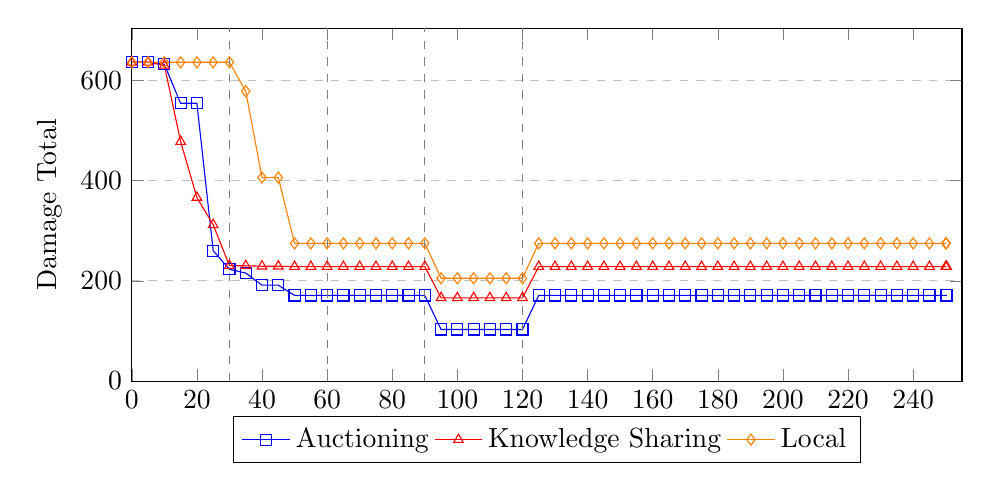
\begin{tikzpicture}
\begin{axis}[
    xlabel={Timestamp [s]},
    ylabel={Damage Total},
    xmin=0, xmax=255000,
    ymin=0, ymax=704,
    legend columns=-1,
    legend style={at={(0.5,-0.1)},anchor=north},
    ymajorgrids=true,
    grid style=dashed,
    width=\textwidth,
    height=0.5\textwidth,
    scaled x ticks=base 10:-3,
    xtick scale label code/.code={}
]

	\addplot[color=blue,mark=square] coordinates {
        (0,636.01)(5000,636.01)(10000,632.06)(15000,554.22)(20000,554.22)(25000,260.13)(30000,223.01)(35000,215.48)(40000,191.39)(45000,191.39)(50000,170.85)(55000,170.85)(60000,170.85)(65000,170.85)(70000,170.85)(75000,170.85)(80000,170.85)(85000,170.85)(90000,170.85)(95000,102.93)(100000,102.93)(105000,102.93)(110000,102.93)(115000,102.93)(120000,102.93)(125000,170.85)(130000,170.85)(135000,170.85)(140000,170.85)(145000,170.85)(150000,170.85)(155000,170.85)(160000,170.85)(165000,170.85)(170000,170.85)(175000,170.85)(180000,170.85)(185000,170.85)(190000,170.85)(195000,170.85)(200000,170.85)(205000,170.85)(210000,170.85)(215000,170.85)(220000,170.85)(225000,170.85)(230000,170.85)(235000,170.85)(240000,170.85)(245000,170.85)(250000,170.85)(250367,170.85)
    };
    \addlegendentry{Auctioning}
	\addplot[color=red,mark=triangle] coordinates {
        (0,636.01)(5000,636.01)(10000,629.93)(15000,477.78)(20000,366.27)(25000,311.79)(30000,230.29)(35000,230.02)(40000,229.15)(45000,229.15)(50000,228.42)(55000,228.42)(60000,228.42)(65000,228.42)(70000,228.42)(75000,228.42)(80000,228.42)(85000,228.42)(90000,228.42)(95000,166.07)(100000,166.07)(105000,166.07)(110000,166.07)(115000,166.07)(120000,166.07)(125000,228.42)(130000,228.42)(135000,228.42)(140000,228.42)(145000,228.42)(150000,228.42)(155000,228.42)(160000,228.42)(165000,228.42)(170000,228.42)(175000,228.42)(180000,228.42)(185000,228.42)(190000,228.42)(195000,228.42)(200000,228.42)(205000,228.42)(210000,228.42)(215000,228.42)(220000,228.42)(225000,228.42)(230000,228.42)(235000,228.42)(240000,228.42)(245000,228.42)(250000,228.42)(250281,228.42)
    };
    \addlegendentry{Knowledge Sharing}
	\addplot[color=orange,mark=diamond] coordinates {
        (0,636.01)(5000,636.01)(10000,636.01)(15000,636.01)(20000,636.01)(25000,636.01)(30000,636.01)(35000,578.19)(40000,406.04)(45000,406.04)(50000,274.81)(55000,274.81)(60000,274.81)(65000,274.81)(70000,274.81)(75000,274.81)(80000,274.81)(85000,274.81)(90000,274.81)(95000,205.14)(100000,205.14)(105000,205.14)(110000,205.14)(115000,205.14)(120000,205.14)(125000,274.81)(130000,274.81)(135000,274.81)(140000,274.81)(145000,274.81)(150000,274.81)(155000,274.81)(160000,274.81)(165000,274.81)(170000,274.81)(175000,274.81)(180000,274.81)(185000,274.81)(190000,274.81)(195000,274.81)(200000,274.81)(205000,274.81)(210000,274.81)(215000,274.81)(220000,274.81)(225000,274.81)(230000,274.81)(235000,274.81)(240000,274.81)(245000,274.81)(250000,274.81)(250187,274.81)
    };
    \addlegendentry{Local}

	\addplot[color=gray, dashed,] coordinates {(30000,0) (30000,704)};
	\addplot[color=gray, dashed,] coordinates {(60000,0) (60000,704)};
	\addplot[color=gray, dashed,] coordinates {(90000,0) (90000,704)};
	\addplot[color=gray, dashed,] coordinates {(120000,0) (120000,704)};


\end{axis}
\end{tikzpicture}
    \caption{This graph shows the overall damage of the system in the unstable scenario. The damage is shown for each of the three strategies. The vertical lines indicate the time at which a node was removed and added again.}
    \label{fig:overall-damage-unstable}
\end{figure}

From this first Figure \ref{fig:overall-damage-unstable} we see a trend that is similar to the one from the first experiment (Figure \ref{fig:overall-damage-no-change}). The second time a node gets removed and then added, we see a small dip in the graphs. But apart from this there are no \emph{new} risks to mitigate as the properties of the nodes do not change. This is also reflected in Figure \ref{fig:messages-unstable}, where the knowledge-sharing agent does not see any property changes (and thus does not send any messages). The auctioning node does send some messages, as perviously due to the attempts of finding adaptations.

\begin{figure}[H]
    \centering
    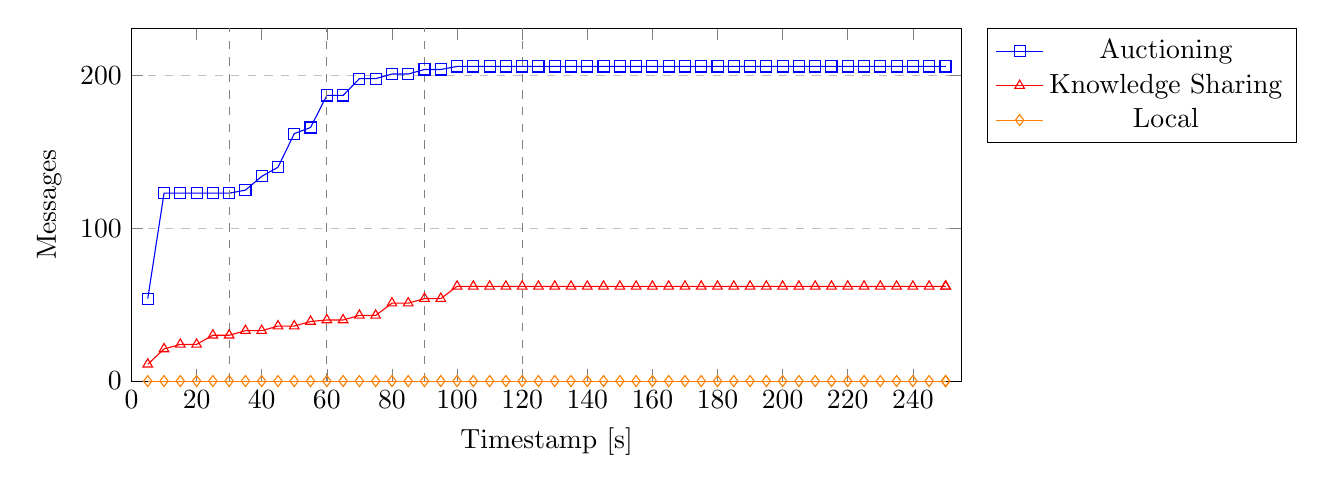
\begin{tikzpicture}
\begin{axis}[
    xlabel={Timestamp [s]},
    ylabel={Messages},
    xmin=0, xmax=255000,
    ymin=0, ymax=231,
    legend pos=outer north east,
    ymajorgrids=true,
    grid style=dashed,
    width=\textwidth,
    height=0.5\textwidth,
    scaled x ticks=base 10:-3,
    xtick scale label code/.code={}
]

	\addplot[color=blue,mark=square] coordinates {
        (5000,54)(10000,123)(15000,123)(20000,123)(25000,123)(30000,123)(35000,125)(40000,134)(45000,140)(50000,162)(55000,166)(60000,187)(65000,187)(70000,198)(75000,198)(80000,201)(85000,201)(90000,204)(95000,204)(100000,206)(105000,206)(110000,206)(115000,206)(120000,206)(125000,206)(130000,206)(135000,206)(140000,206)(145000,206)(150000,206)(155000,206)(160000,206)(165000,206)(170000,206)(175000,206)(180000,206)(185000,206)(190000,206)(195000,206)(200000,206)(205000,206)(210000,206)(215000,206)(220000,206)(225000,206)(230000,206)(235000,206)(240000,206)(245000,206)(250000,206)(250128,206)
    };
    \addlegendentry{Auctioning}
	\addplot[color=red,mark=triangle] coordinates {
        (5000,11)(10000,21)(15000,24)(20000,24)(25000,30)(30000,30)(35000,33)(40000,33)(45000,36)(50000,36)(55000,39)(60000,40)(65000,40)(70000,43)(75000,43)(80000,51)(85000,51)(90000,54)(95000,54)(100000,62)(105000,62)(110000,62)(115000,62)(120000,62)(125000,62)(130000,62)(135000,62)(140000,62)(145000,62)(150000,62)(155000,62)(160000,62)(165000,62)(170000,62)(175000,62)(180000,62)(185000,62)(190000,62)(195000,62)(200000,62)(205000,62)(210000,62)(215000,62)(220000,62)(225000,62)(230000,62)(235000,62)(240000,62)(245000,62)(250000,62)(250118,62)
    };
    \addlegendentry{Knowledge Sharing}
	\addplot[color=orange,mark=diamond] coordinates {
        (5000,0)(10000,0)(15000,0)(20000,0)(25000,0)(30000,0)(35000,0)(40000,0)(45000,0)(50000,0)(55000,0)(60000,0)(65000,0)(70000,0)(75000,0)(80000,0)(85000,0)(90000,0)(95000,0)(100000,0)(105000,0)(110000,0)(115000,0)(120000,0)(125000,0)(130000,0)(135000,0)(140000,0)(145000,0)(150000,0)(155000,0)(160000,0)(165000,0)(170000,0)(175000,0)(180000,0)(185000,0)(190000,0)(195000,0)(200000,0)(205000,0)(210000,0)(215000,0)(220000,0)(225000,0)(230000,0)(235000,0)(240000,0)(245000,0)(250000,0)(250107,0)
    };
    \addlegendentry{Local}

	\addplot[color=gray, dashed,] coordinates {(30000,0) (30000,231)};
	\addplot[color=gray, dashed,] coordinates {(60000,0) (60000,231)};
	\addplot[color=gray, dashed,] coordinates {(90000,0) (90000,231)};
	\addplot[color=gray, dashed,] coordinates {(120000,0) (120000,231)};


\end{axis}
\end{tikzpicture}
    \caption{Graph showing the total amount of messages sent between agents in the unstable scenario.}
    \label{fig:messages-unstable}
\end{figure}

\begin{figure}[H]
    \centering
    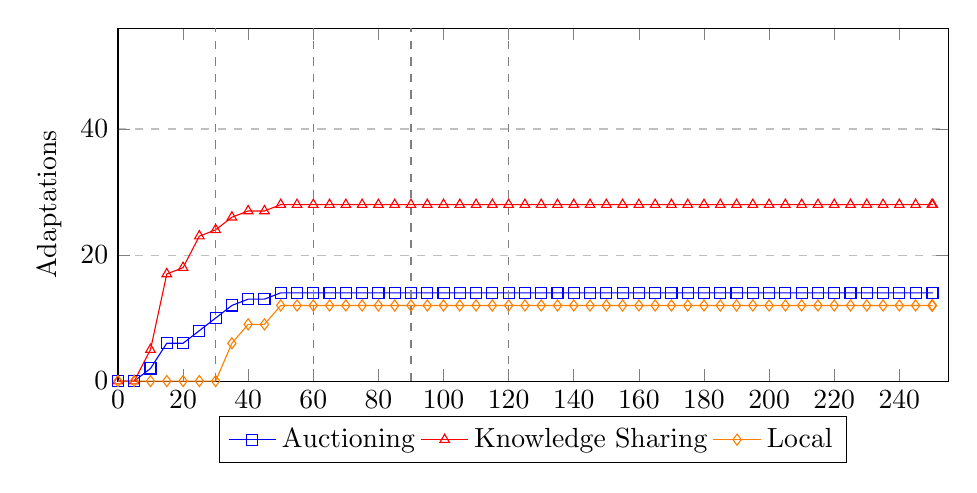
\begin{tikzpicture}
\begin{axis}[
    xlabel={Timestamp [s]},
    ylabel={Adaptations},
    xmin=0, xmax=255000,
    ymin=0, ymax=56,
    legend columns=-1,
    legend style={at={(0.5,-0.1)},anchor=north},
    ymajorgrids=true,
    grid style=dashed,
    width=\textwidth,
    height=0.5\textwidth,
    scaled x ticks=base 10:-3,
    xtick scale label code/.code={}
]

	\addplot[color=blue,mark=square] coordinates {
        (0,0)(5000,0)(10000,2)(15000,6)(20000,6)(25000,8)(30000,10)(35000,12)(40000,13)(45000,13)(50000,14)(55000,14)(60000,14)(65000,14)(70000,14)(75000,14)(80000,14)(85000,14)(90000,14)(95000,14)(100000,14)(105000,14)(110000,14)(115000,14)(120000,14)(125000,14)(130000,14)(135000,14)(140000,14)(145000,14)(150000,14)(155000,14)(160000,14)(165000,14)(170000,14)(175000,14)(180000,14)(185000,14)(190000,14)(195000,14)(200000,14)(205000,14)(210000,14)(215000,14)(220000,14)(225000,14)(230000,14)(235000,14)(240000,14)(245000,14)(250000,14)(250367,14)
    };
    \addlegendentry{Auctioning}
	\addplot[color=red,mark=triangle] coordinates {
        (0,0)(5000,0)(10000,5)(15000,17)(20000,18)(25000,23)(30000,24)(35000,26)(40000,27)(45000,27)(50000,28)(55000,28)(60000,28)(65000,28)(70000,28)(75000,28)(80000,28)(85000,28)(90000,28)(95000,28)(100000,28)(105000,28)(110000,28)(115000,28)(120000,28)(125000,28)(130000,28)(135000,28)(140000,28)(145000,28)(150000,28)(155000,28)(160000,28)(165000,28)(170000,28)(175000,28)(180000,28)(185000,28)(190000,28)(195000,28)(200000,28)(205000,28)(210000,28)(215000,28)(220000,28)(225000,28)(230000,28)(235000,28)(240000,28)(245000,28)(250000,28)(250281,28)
    };
    \addlegendentry{Knowledge Sharing}
	\addplot[color=orange,mark=diamond] coordinates {
        (0,0)(5000,0)(10000,0)(15000,0)(20000,0)(25000,0)(30000,0)(35000,6)(40000,9)(45000,9)(50000,12)(55000,12)(60000,12)(65000,12)(70000,12)(75000,12)(80000,12)(85000,12)(90000,12)(95000,12)(100000,12)(105000,12)(110000,12)(115000,12)(120000,12)(125000,12)(130000,12)(135000,12)(140000,12)(145000,12)(150000,12)(155000,12)(160000,12)(165000,12)(170000,12)(175000,12)(180000,12)(185000,12)(190000,12)(195000,12)(200000,12)(205000,12)(210000,12)(215000,12)(220000,12)(225000,12)(230000,12)(235000,12)(240000,12)(245000,12)(250000,12)(250187,12)
    };
    \addlegendentry{Local}

	\addplot[color=gray, dashed,] coordinates {(30000,0) (30000,56)};
	\addplot[color=gray, dashed,] coordinates {(60000,0) (60000,56)};
	\addplot[color=gray, dashed,] coordinates {(90000,0) (90000,56)};
	\addplot[color=gray, dashed,] coordinates {(120000,0) (120000,56)};


\end{axis}
\end{tikzpicture}
    \caption{Graph showing the total amount of adaptations applied by agents in the unstable scenario.}
    \label{fig:proposals-unstable}
\end{figure}

Figure \ref{fig:proposals-unstable} is similar to the \emph{No change} scenario (Figure \ref{fig:proposals-no-change}), and is inline with the damage reduction visible in Figure \ref{fig:overall-damage-unstable}. No new adaptations are applied, and the infrastructure remains stable. The agents also do not detect any new risks, as the properties remain the same. This is reflected in Figure \ref{fig:risk-count-unstable} and \ref{fig:risk-remaining-unstable}.

\begin{figure}[H]
    \centering
        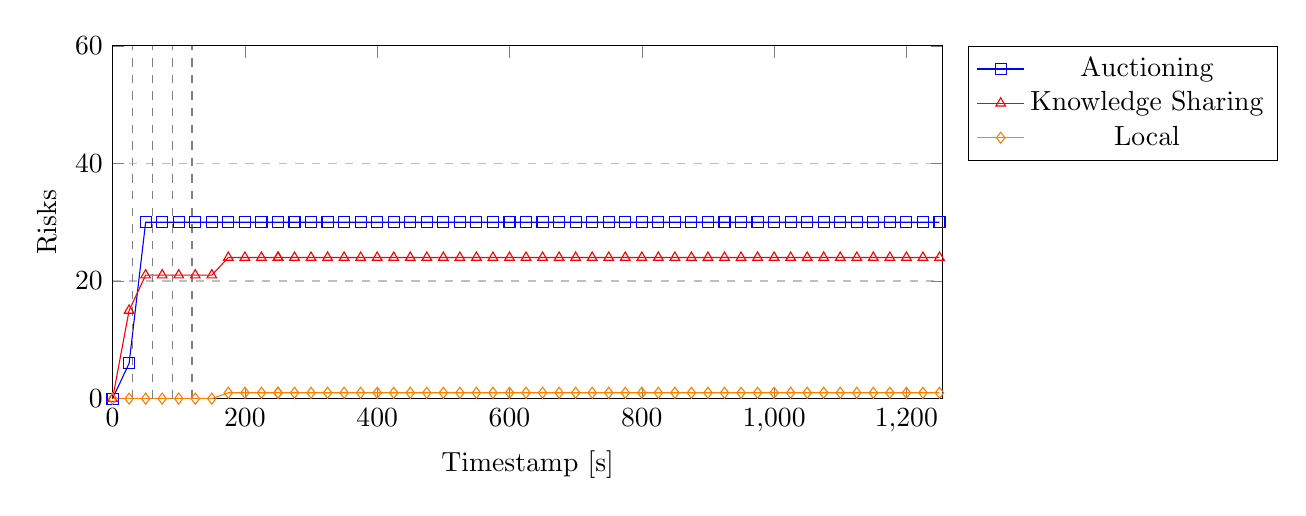
\begin{tikzpicture}
\begin{axis}[
    xlabel={Timestamp [s]},
    ylabel={Risks},
    xmin=0, xmax=1255000,
    ymin=0, ymax=60,
    legend pos=outer north east,
    ymajorgrids=true,
    grid style=dashed,
    width=\textwidth,
    height=0.5\textwidth,
    scaled x ticks=base 10:-3,
    xtick scale label code/.code={}
]

	\addplot[color=blue,mark=square] coordinates {
        (0,0)(25000,6)(50000,30)(75000,30)(100000,30)(125000,30)(150000,30)(175000,30)(200000,30)(225000,30)(250000,30)(275000,30)(300000,30)(325000,30)(350000,30)(375000,30)(400000,30)(425000,30)(450000,30)(475000,30)(500000,30)(525000,30)(550000,30)(575000,30)(600000,30)(625000,30)(650000,30)(675000,30)(700000,30)(725000,30)(750000,30)(775000,30)(800000,30)(825000,30)(850000,30)(875000,30)(900000,30)(925000,30)(950000,30)(975000,30)(1000000,30)(1025000,30)(1050000,30)(1075000,30)(1100000,30)(1125000,30)(1150000,30)(1175000,30)(1200000,30)(1225000,30)(1250000,30)(250362,30)
    };
    \addlegendentry{Auctioning}
	\addplot[color=red,mark=triangle] coordinates {
        (0,0)(25000,15)(50000,21)(75000,21)(100000,21)(125000,21)(150000,21)(175000,24)(200000,24)(225000,24)(250000,24)(275000,24)(300000,24)(325000,24)(350000,24)(375000,24)(400000,24)(425000,24)(450000,24)(475000,24)(500000,24)(525000,24)(550000,24)(575000,24)(600000,24)(625000,24)(650000,24)(675000,24)(700000,24)(725000,24)(750000,24)(775000,24)(800000,24)(825000,24)(850000,24)(875000,24)(900000,24)(925000,24)(950000,24)(975000,24)(1000000,24)(1025000,24)(1050000,24)(1075000,24)(1100000,24)(1125000,24)(1150000,24)(1175000,24)(1200000,24)(1225000,24)(1250000,24)(250334,24)
    };
    \addlegendentry{Knowledge Sharing}
	\addplot[color=orange,mark=diamond] coordinates {
        (0,0)(25000,0)(50000,0)(75000,0)(100000,0)(125000,0)(150000,0)(175000,1)(200000,1)(225000,1)(250000,1)(275000,1)(300000,1)(325000,1)(350000,1)(375000,1)(400000,1)(425000,1)(450000,1)(475000,1)(500000,1)(525000,1)(550000,1)(575000,1)(600000,1)(625000,1)(650000,1)(675000,1)(700000,1)(725000,1)(750000,1)(775000,1)(800000,1)(825000,1)(850000,1)(875000,1)(900000,1)(925000,1)(950000,1)(975000,1)(1000000,1)(1025000,1)(1050000,1)(1075000,1)(1100000,1)(1125000,1)(1150000,1)(1175000,1)(1200000,1)(1225000,1)(1250000,1)(250168,1)
    };
    \addlegendentry{Local}

	\addplot[color=gray, dashed,] coordinates {(30000,0) (30000,60)};
	\addplot[color=gray, dashed,] coordinates {(60000,0) (60000,60)};
	\addplot[color=gray, dashed,] coordinates {(90000,0) (90000,60)};
	\addplot[color=gray, dashed,] coordinates {(120000,0) (120000,60)};


\end{axis}
\end{tikzpicture}
    \caption{Graph showing the number of unique risks detected by agents in the unstable scenario.}
    \label{fig:risk-count-unstable}
\end{figure}

\begin{figure}[H]
    \centering
        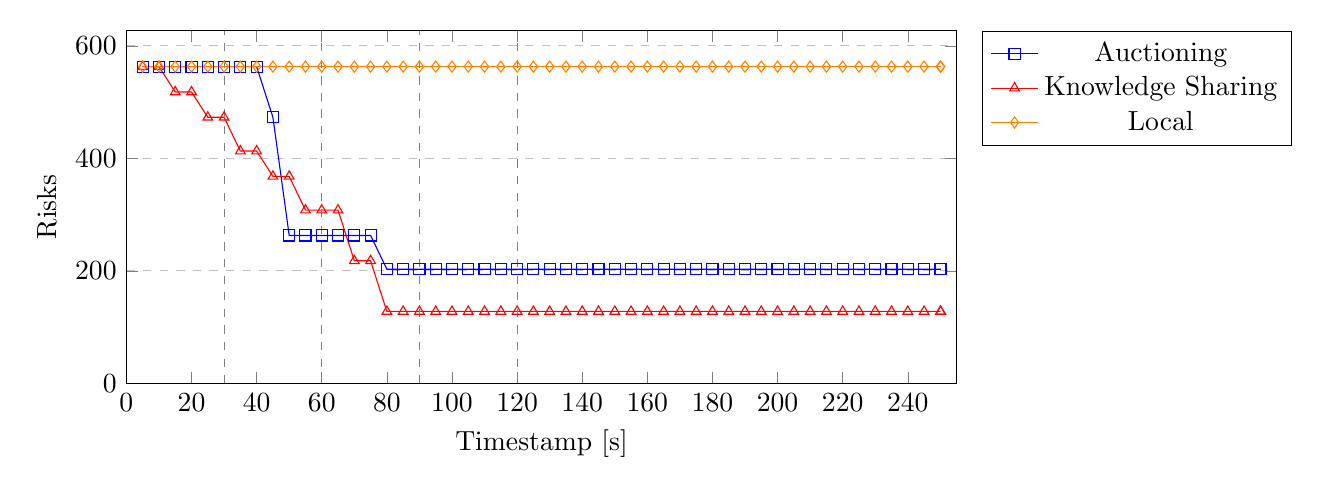
\begin{tikzpicture}
\begin{axis}[
    xlabel={Timestamp [s]},
    ylabel={Risks},
    xmin=0, xmax=255000,
    ymin=0, ymax=627,
    legend pos=outer north east,
    ymajorgrids=true,
    grid style=dashed,
    width=\textwidth,
    height=0.5\textwidth,
    scaled x ticks=base 10:-3,
    xtick scale label code/.code={}
]

	\addplot[color=blue,mark=square] coordinates {
        (5000,563)(10000,563)(15000,563)(20000,563)(25000,563)(30000,563)(35000,563)(40000,563)(45000,473)(50000,263)(55000,263)(60000,263)(65000,263)(70000,263)(75000,263)(80000,203)(85000,203)(90000,203)(95000,203)(100000,203)(105000,203)(110000,203)(115000,203)(120000,203)(125000,203)(130000,203)(135000,203)(140000,203)(145000,203)(150000,203)(155000,203)(160000,203)(165000,203)(170000,203)(175000,203)(180000,203)(185000,203)(190000,203)(195000,203)(200000,203)(205000,203)(210000,203)(215000,203)(220000,203)(225000,203)(230000,203)(235000,203)(240000,203)(245000,203)(250000,203)(250128,203)
    };
    \addlegendentry{Auctioning}
	\addplot[color=red,mark=triangle] coordinates {
        (5000,563)(10000,563)(15000,518)(20000,518)(25000,473)(30000,473)(35000,413)(40000,413)(45000,368)(50000,368)(55000,308)(60000,308)(65000,308)(70000,218)(75000,218)(80000,128)(85000,128)(90000,128)(95000,128)(100000,128)(105000,128)(110000,128)(115000,128)(120000,128)(125000,128)(130000,128)(135000,128)(140000,128)(145000,128)(150000,128)(155000,128)(160000,128)(165000,128)(170000,128)(175000,128)(180000,128)(185000,128)(190000,128)(195000,128)(200000,128)(205000,128)(210000,128)(215000,128)(220000,128)(225000,128)(230000,128)(235000,128)(240000,128)(245000,128)(250000,128)(250118,128)
    };
    \addlegendentry{Knowledge Sharing}
	\addplot[color=orange,mark=diamond] coordinates {
        (5000,563)(10000,563)(15000,563)(20000,563)(25000,563)(30000,563)(35000,563)(40000,563)(45000,563)(50000,563)(55000,563)(60000,563)(65000,563)(70000,563)(75000,563)(80000,563)(85000,563)(90000,563)(95000,563)(100000,563)(105000,563)(110000,563)(115000,563)(120000,563)(125000,563)(130000,563)(135000,563)(140000,563)(145000,563)(150000,563)(155000,563)(160000,563)(165000,563)(170000,563)(175000,563)(180000,563)(185000,563)(190000,563)(195000,563)(200000,563)(205000,563)(210000,563)(215000,563)(220000,563)(225000,563)(230000,563)(235000,563)(240000,563)(245000,563)(250000,563)(250107,563)
    };
    \addlegendentry{Local}

	\addplot[color=gray, dashed,] coordinates {(30000,0) (30000,627)};
	\addplot[color=gray, dashed,] coordinates {(60000,0) (60000,627)};
	\addplot[color=gray, dashed,] coordinates {(90000,0) (90000,627)};
	\addplot[color=gray, dashed,] coordinates {(120000,0) (120000,627)};


\end{axis}
\end{tikzpicture}
    \caption{Graph showing the number of remaining risks in the infrastructure in the unstable scenario.}
    \label{fig:risk-remaining-unstable}
\end{figure}

\add{write}

\begin{figure}[H]
    \centering
        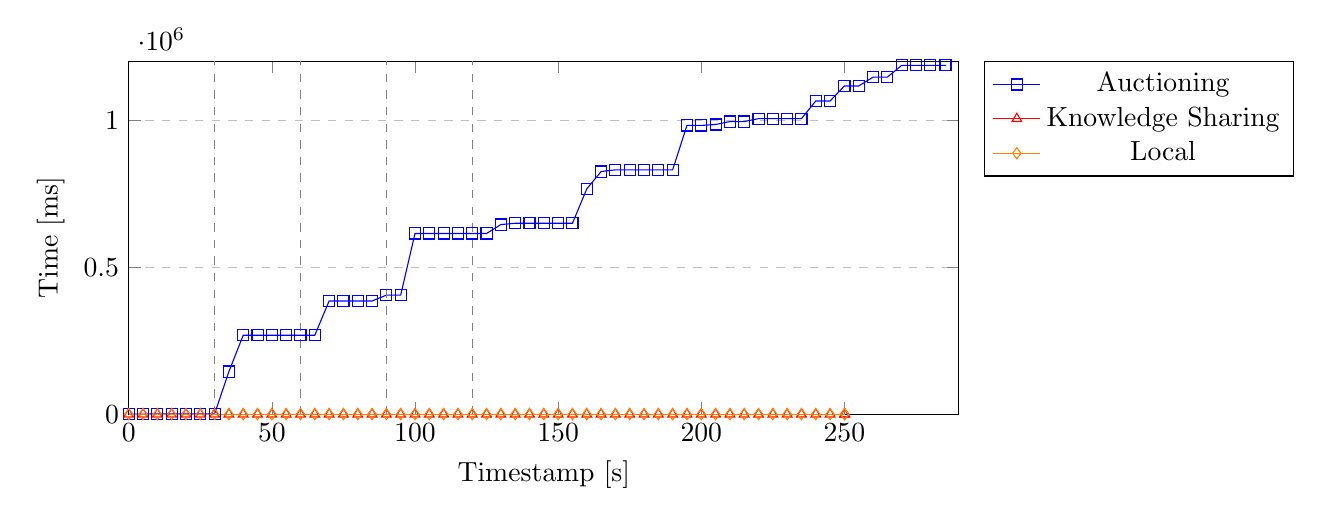
\begin{tikzpicture}
\begin{axis}[
    xlabel={Timestamp [s]},
    ylabel={Time [ms]},
    xmin=0, xmax=290000,
    ymin=0, ymax=1200012,
    legend pos=outer north east,
    ymajorgrids=true,
    grid style=dashed,
    width=\textwidth,
    height=0.5\textwidth,
    scaled x ticks=base 10:-3,
    xtick scale label code/.code={}
]

	\addplot[color=blue,mark=square] coordinates {
        (0,0)(5000,138)(10000,1198)(15000,1198)(20000,1198)(25000,1207)(30000,1207)(35000,144954)(40000,268597)(45000,268597)(50000,268597)(55000,268597)(60000,268597)(65000,268597)(70000,384913)(75000,384913)(80000,384919)(85000,384919)(90000,404941)(95000,404941)(100000,614605)(105000,614605)(110000,614608)(115000,614608)(120000,614609)(125000,614609)(130000,644926)(135000,649250)(140000,649250)(145000,649250)(150000,649251)(155000,649251)(160000,766138)(165000,825152)(170000,831011)(175000,831011)(180000,831012)(185000,831012)(190000,831012)(195000,982057)(200000,982057)(205000,985177)(210000,995185)(215000,995185)(220000,1005197)(225000,1005197)(230000,1005197)(235000,1005197)(240000,1065215)(245000,1065215)(250000,1116271)(255000,1116271)(260000,1146280)(265000,1146280)(270000,1186297)(275000,1186297)(280000,1186297)(285000,1186297)(285530,1186297)
    };
    \addlegendentry{Auctioning}
	\addplot[color=red,mark=triangle] coordinates {
        (0,0)(5000,0)(10000,0)(15000,0)(20000,0)(25000,0)(30000,0)(35000,0)(40000,0)(45000,0)(50000,0)(55000,0)(60000,0)(65000,0)(70000,0)(75000,0)(80000,0)(85000,0)(90000,0)(95000,0)(100000,0)(105000,0)(110000,0)(115000,0)(120000,0)(125000,0)(130000,0)(135000,0)(140000,0)(145000,0)(150000,0)(155000,0)(160000,0)(165000,0)(170000,0)(175000,0)(180000,0)(185000,0)(190000,0)(195000,0)(200000,0)(205000,0)(210000,0)(215000,0)(220000,0)(225000,0)(230000,0)(235000,0)(240000,0)(245000,0)(250000,0)(250138,0)
    };
    \addlegendentry{Knowledge Sharing}
	\addplot[color=orange,mark=diamond] coordinates {
        (0,0)(5000,0)(10000,0)(15000,0)(20000,0)(25000,0)(30000,0)(35000,0)(40000,0)(45000,0)(50000,0)(55000,0)(60000,0)(65000,0)(70000,0)(75000,0)(80000,0)(85000,0)(90000,0)(95000,0)(100000,0)(105000,0)(110000,0)(115000,0)(120000,0)(125000,0)(130000,0)(135000,0)(140000,0)(145000,0)(150000,0)(155000,0)(160000,0)(165000,0)(170000,0)(175000,0)(180000,0)(185000,0)(190000,0)(195000,0)(200000,0)(205000,0)(210000,0)(215000,0)(220000,0)(225000,0)(230000,0)(235000,0)(240000,0)(245000,0)(250000,0)(250134,0)
    };
    \addlegendentry{Local}

	\addplot[color=gray, dashed,] coordinates {(30000,0) (30000,1200012)};
	\addplot[color=gray, dashed,] coordinates {(60000,0) (60000,1200012)};
	\addplot[color=gray, dashed,] coordinates {(90000,0) (90000,1200012)};
	\addplot[color=gray, dashed,] coordinates {(120000,0) (120000,1200012)};


\end{axis}
\end{tikzpicture}
    \caption{Graph showing the sum of time spent auctioning by agents in the unstable scenario.}
    \label{fig:auctioning-time-unstable}
\end{figure}

\begin{figure}[H]
    \centering
        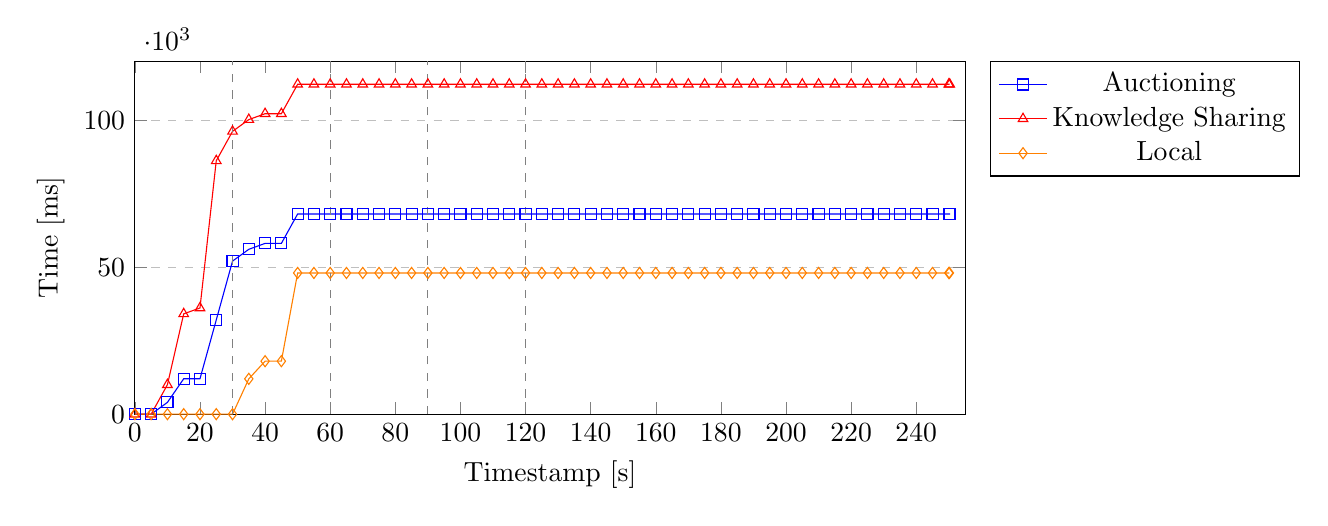
\begin{tikzpicture}
\begin{axis}[
    xlabel={Timestamp [s]},
    ylabel={Time [ms]},
    xmin=0, xmax=255000,
    ymin=0, ymax=120012,
    legend pos=outer north east,
    ymajorgrids=true,
    grid style=dashed,
    width=\textwidth,
    height=0.5\textwidth,
    scaled x ticks=base 10:-3,
    scaled y ticks=base 10:-3,
    xtick scale label code/.code={}
]

	\addplot[color=blue,mark=square] coordinates {
        (0,0)(5000,0)(10000,4012)(15000,12040)(20000,12040)(25000,32049)(30000,52060)(35000,56077)(40000,58088)(45000,58088)(50000,68099)(55000,68099)(60000,68099)(65000,68099)(70000,68099)(75000,68099)(80000,68099)(85000,68099)(90000,68099)(95000,68099)(100000,68099)(105000,68099)(110000,68099)(115000,68099)(120000,68099)(125000,68099)(130000,68099)(135000,68099)(140000,68099)(145000,68099)(150000,68099)(155000,68099)(160000,68099)(165000,68099)(170000,68099)(175000,68099)(180000,68099)(185000,68099)(190000,68099)(195000,68099)(200000,68099)(205000,68099)(210000,68099)(215000,68099)(220000,68099)(225000,68099)(230000,68099)(235000,68099)(240000,68099)(245000,68099)(250000,68099)(250367,68099)
    };
    \addlegendentry{Auctioning}
	\addplot[color=red,mark=triangle] coordinates {
        (0,0)(5000,0)(10000,10030)(15000,34121)(20000,36123)(25000,86181)(30000,96189)(35000,100197)(40000,102199)(45000,102199)(50000,112207)(55000,112207)(60000,112207)(65000,112207)(70000,112207)(75000,112207)(80000,112207)(85000,112207)(90000,112207)(95000,112207)(100000,112207)(105000,112207)(110000,112207)(115000,112207)(120000,112207)(125000,112207)(130000,112207)(135000,112207)(140000,112207)(145000,112207)(150000,112207)(155000,112207)(160000,112207)(165000,112207)(170000,112207)(175000,112207)(180000,112207)(185000,112207)(190000,112207)(195000,112207)(200000,112207)(205000,112207)(210000,112207)(215000,112207)(220000,112207)(225000,112207)(230000,112207)(235000,112207)(240000,112207)(245000,112207)(250000,112207)(250281,112207)
    };
    \addlegendentry{Knowledge Sharing}
	\addplot[color=orange,mark=diamond] coordinates {
        (0,0)(5000,0)(10000,0)(15000,0)(20000,0)(25000,0)(30000,0)(35000,12019)(40000,18027)(45000,18027)(50000,48034)(55000,48034)(60000,48034)(65000,48034)(70000,48034)(75000,48034)(80000,48034)(85000,48034)(90000,48034)(95000,48034)(100000,48034)(105000,48034)(110000,48034)(115000,48034)(120000,48034)(125000,48034)(130000,48034)(135000,48034)(140000,48034)(145000,48034)(150000,48034)(155000,48034)(160000,48034)(165000,48034)(170000,48034)(175000,48034)(180000,48034)(185000,48034)(190000,48034)(195000,48034)(200000,48034)(205000,48034)(210000,48034)(215000,48034)(220000,48034)(225000,48034)(230000,48034)(235000,48034)(240000,48034)(245000,48034)(250000,48034)(250187,48034)
    };
    \addlegendentry{Local}

	\addplot[color=gray, dashed,] coordinates {(30000,0) (30000,120012)};
	\addplot[color=gray, dashed,] coordinates {(60000,0) (60000,120012)};
	\addplot[color=gray, dashed,] coordinates {(90000,0) (90000,120012)};
	\addplot[color=gray, dashed,] coordinates {(120000,0) (120000,120012)};


\end{axis}
\end{tikzpicture}

    \caption{Graph showing the sum of time spent adapting by agents in the unstable scenario.}
    \label{fig:adapting-time-unstable}
\end{figure}

As with the prior graphs for this scenario we see that Figure \ref{fig:adapting-time-unstable} is also stable after the first $50$ seconds. There are no new risks as shown in Figure \ref{fig:risk-count-unstable} and no new adaptations are necessary to mitigate them. 



\subsection*{Consecutive runs}
\begin{figure}[H]
    \centering
        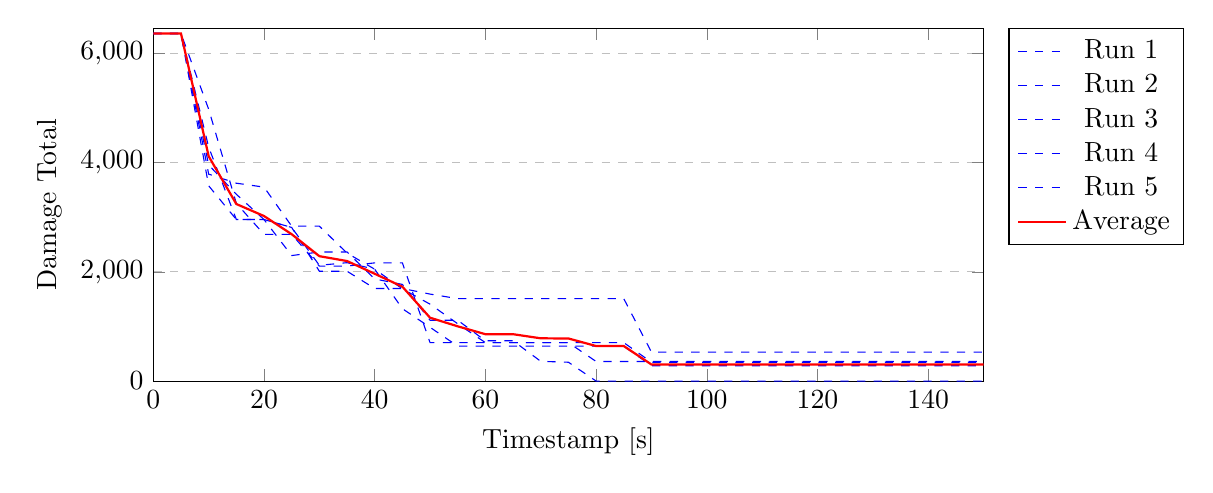
\begin{tikzpicture}
\begin{axis}[
    xlabel={Timestamp [s]},
    ylabel={Damage Total},
    xmin=0, xmax=150000,
    ymin=0, ymax=6464,
    legend pos=outer north east,
    ymajorgrids=true,
    grid style=dashed,
    width=\textwidth,
    height=0.5\textwidth,
    scaled x ticks=base 10:-3,
    xtick scale label code/.code={}
]

\addplot[dashed,color=blue] coordinates {
    (0,6367.26)(5000,6367.26)(10000,4979.76)(15000,3254.95)(20000,2688.57)(25000,2688.57)(30000,2106.11)(35000,2106.11)(40000,2165.47)(45000,2165.47)(50000,704.40)(55000,704.40)(60000,704.40)(65000,704.40)(70000,704.40)(75000,704.40)(80000,704.40)(85000,704.40)(90000,345.19)(95000,345.19)(100000,345.19)(105000,345.19)(110000,345.19)(115000,345.19)(120000,345.19)(125000,345.19)(130000,345.19)(135000,345.19)(140000,345.19)(145000,345.19)(150000,345.19)(155000,345.19)(160000,345.19)(165000,345.19)(170000,345.19)(175000,345.19)(180000,345.19)(185000,345.19)(190000,345.19)(195000,345.19)(200000,345.19)(205000,345.19)(210000,345.19)(215000,345.19)(220000,345.19)(225000,345.19)(230000,345.19)(235000,345.19)(240000,345.19)(245000,345.19)(250000,345.19)(255000,345.19)(260000,345.19)(265000,345.19)(270000,345.19)(275000,345.19)(280000,345.19)(285000,345.19)(290000,345.19)(295000,345.19)(300000,345.19)(305000,345.19)(310000,345.19)(315000,345.19)(316684,345.19)
};
\addlegendentry{Run 1}
\addplot[dashed,color=blue] coordinates {
    (0,6367.26)(5000,6367.26)(10000,3960.57)(15000,3421.82)(20000,2959.69)(25000,2813.83)(30000,2012.56)(35000,2012.56)(40000,1696.12)(45000,1696.12)(50000,1593.65)(55000,1509.99)(60000,1509.99)(65000,1509.99)(70000,1509.99)(75000,1509.99)(80000,1509.99)(85000,1509.99)(90000,530.56)(95000,530.56)(100000,530.56)(105000,530.56)(110000,530.56)(115000,530.56)(120000,530.56)(125000,530.56)(130000,530.56)(135000,530.56)(140000,530.56)(145000,530.56)(150000,530.56)(155000,530.56)(160000,530.56)(165000,530.56)(170000,530.56)(175000,530.56)(180000,530.56)(185000,530.56)(190000,530.56)(195000,530.56)(200000,530.56)(205000,530.56)(210000,530.56)(215000,530.56)(220000,530.56)(225000,530.56)(230000,530.56)(235000,530.56)(240000,530.56)(245000,530.56)(250000,530.56)(255000,530.56)(260000,530.56)(265000,530.56)(270000,530.56)(275000,530.56)(280000,530.56)(285000,530.56)(290000,530.56)(295000,530.56)(300000,530.56)(305000,530.56)(310000,530.56)(315000,530.56)(320000,530.56)(322398,530.56)
};
\addlegendentry{Run 2}
\addplot[dashed,color=blue] coordinates {
    (0,6367.26)(5000,6367.26)(10000,3790.83)(15000,3624.89)(20000,3553.25)(25000,2838.03)(30000,2838.03)(35000,2344.39)(40000,2049.23)(45000,1689.44)(50000,1408.80)(55000,1049.59)(60000,704.40)(65000,704.40)(70000,704.40)(75000,704.40)(80000,359.22)(85000,359.22)(90000,359.22)(95000,359.22)(100000,359.22)(105000,359.22)(110000,359.22)(115000,359.22)(120000,359.22)(125000,359.22)(130000,359.22)(135000,359.22)(140000,359.22)(145000,359.22)(150000,359.22)(155000,359.22)(160000,359.22)(165000,359.22)(170000,359.22)(175000,359.22)(180000,359.22)(185000,359.22)(190000,359.22)(195000,359.22)(200000,359.22)(205000,359.22)(210000,359.22)(215000,359.22)(220000,359.22)(225000,359.22)(230000,359.22)(235000,359.22)(240000,359.22)(245000,359.22)(250000,359.22)(255000,359.22)(260000,359.22)(265000,359.22)(270000,359.22)(275000,359.22)(280000,359.22)(285000,359.22)(290000,359.22)(295000,359.22)(300000,359.22)(305000,359.22)(310000,359.22)(310174,359.22)
};
\addlegendentry{Run 3}
\addplot[dashed,color=blue] coordinates {
    (0,6367.26)(5000,6367.26)(10000,3577.98)(15000,2959.69)(20000,2959.69)(25000,2299.49)(30000,2364.62)(35000,2364.62)(40000,1870.16)(45000,1770.67)(50000,1114.75)(55000,1114.75)(60000,738.27)(65000,738.27)(70000,361.78)(75000,345.19)(80000,0.00)(85000,0.00)(90000,0.00)(95000,0.00)(100000,0.00)(105000,0.00)(110000,0.00)(115000,0.00)(120000,0.00)(125000,0.00)(130000,0.00)(135000,0.00)(140000,0.00)(145000,0.00)(150000,0.00)(155000,0.00)(160000,0.00)(165000,0.00)(170000,0.00)(175000,0.00)(180000,0.00)(185000,0.00)(190000,0.00)(195000,0.00)(200000,0.00)(205000,0.00)(210000,0.00)(215000,0.00)(220000,0.00)(225000,0.00)(230000,0.00)(235000,0.00)(240000,0.00)(245000,0.00)(250000,0.00)(255000,0.00)(260000,0.00)(265000,0.00)(270000,0.00)(275000,0.00)(280000,0.00)(285000,0.00)(290000,0.00)(295000,0.00)(300000,0.00)(305000,0.00)(310000,0.00)(315000,0.00)(318260,0.00)
};
\addlegendentry{Run 4}
\addplot[dashed,color=blue] coordinates {
    (0,6367.26)(5000,6367.26)(10000,4286.53)(15000,2959.69)(20000,2959.69)(25000,2813.83)(30000,2120.54)(35000,2169.05)(40000,2049.23)(45000,1326.65)(50000,985.04)(55000,639.86)(60000,639.86)(65000,639.86)(70000,639.86)(75000,639.86)(80000,639.86)(85000,639.86)(90000,280.64)(95000,280.64)(100000,280.64)(105000,280.64)(110000,280.64)(115000,280.64)(120000,280.64)(125000,280.64)(130000,280.64)(135000,280.64)(140000,280.64)(145000,280.64)(150000,280.64)(155000,280.64)(160000,280.64)(165000,280.64)(170000,280.64)(175000,280.64)(180000,280.64)(185000,280.64)(190000,280.64)(195000,280.64)(200000,280.64)(205000,280.64)(210000,280.64)(215000,280.64)(220000,280.64)(225000,280.64)(230000,280.64)(235000,280.64)(240000,280.64)(245000,280.64)(250000,280.64)(255000,280.64)(260000,280.64)(265000,280.64)(270000,280.64)(275000,280.64)(280000,280.64)(285000,280.64)(290000,280.64)(295000,280.64)(300000,280.64)(305000,280.64)(310000,280.64)(313118,280.64)
};
\addlegendentry{Run 5}
\addplot[thick, color=red] coordinates {
    (0,6367)(5000,6367)(10000,4118.4)(15000,3243.4)(20000,3023.6)(25000,2690.2)(30000,2288)(35000,2199)(40000,1965.8)(45000,1729.2)(50000,1160.8)(55000,1003)(60000,858.8)(65000,858.8)(70000,783.4)(75000,780.2)(80000,642.2)(85000,642.2)(90000,302.8)(95000,302.8)(100000,302.8)(105000,302.8)(110000,302.8)(115000,302.8)(120000,302.8)(125000,302.8)(130000,302.8)(135000,302.8)(140000,302.8)(145000,302.8)(150000,302.8)(155000,302.8)(160000,302.8)(165000,302.8)(170000,302.8)(175000,302.8)(180000,302.8)(185000,302.8)(190000,302.8)(195000,302.8)(200000,302.8)(205000,302.8)(210000,302.8)(215000,302.8)(220000,302.8)(225000,302.8)(230000,302.8)(235000,302.8)(240000,302.8)(245000,302.8)(250000,302.8)(255000,302.8)(260000,302.8)(265000,302.8)(270000,302.8)(275000,302.8)(280000,302.8)(285000,302.8)(290000,302.8)(295000,302.8)(300000,302.8)(305000,302.8)(310000,302.8)(315000,302.8)(316684,NaN)
};
\addlegendentry{Average}

\end{axis}
\end{tikzpicture}

    \caption{Graph showing the Auctioning Feature's performance over multiple runs in the no-change scenario.}
\end{figure}

\subsection*{Small Infrastructure}
\begin{figure}[H]
    \centering
        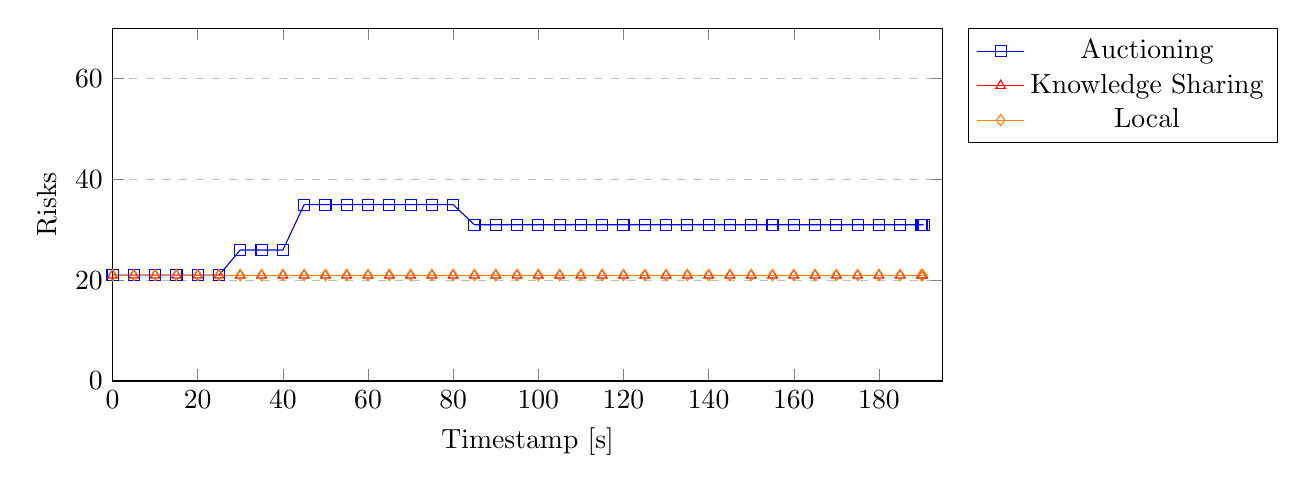
\begin{tikzpicture}
\begin{axis}[
    xlabel={Timestamp [s]},
    ylabel={Risks},
    xmin=0, xmax=195000,
    ymin=0, ymax=70,
    legend pos=outer north east,
    ymajorgrids=true,
    grid style=dashed,
    width=\textwidth,
    height=0.5\textwidth,
    scaled x ticks=base 10:-3,
    xtick scale label code/.code={}
]

	\addplot[color=blue,mark=square] coordinates {
        (0,21)(5000,21)(10000,21)(15000,21)(20000,21)(25000,21)(30000,26)(35000,26)(40000,26)(45000,35)(50000,35)(55000,35)(60000,35)(65000,35)(70000,35)(75000,35)(80000,35)(85000,31)(90000,31)(95000,31)(100000,31)(105000,31)(110000,31)(115000,31)(120000,31)(125000,31)(130000,31)(135000,31)(140000,31)(145000,31)(150000,31)(155000,31)(160000,31)(165000,31)(170000,31)(175000,31)(180000,31)(185000,31)(190000,31)(190477,31)
    };
    \addlegendentry{Auctioning}
	\addplot[color=red,mark=triangle] coordinates {
        (0,21)(5000,21)(10000,21)(15000,21)(20000,21)(25000,21)(30000,21)(35000,21)(40000,21)(45000,21)(50000,21)(55000,21)(60000,21)(65000,21)(70000,21)(75000,21)(80000,21)(85000,21)(90000,21)(95000,21)(100000,21)(105000,21)(110000,21)(115000,21)(120000,21)(125000,21)(130000,21)(135000,21)(140000,21)(145000,21)(150000,21)(155000,21)(160000,21)(165000,21)(170000,21)(175000,21)(180000,21)(185000,21)(190000,21)(190245,21)
    };
    \addlegendentry{Knowledge Sharing}
	\addplot[color=orange,mark=diamond] coordinates {
        (0,21)(5000,21)(10000,21)(15000,21)(20000,21)(25000,21)(30000,21)(35000,21)(40000,21)(45000,21)(50000,21)(55000,21)(60000,21)(65000,21)(70000,21)(75000,21)(80000,21)(85000,21)(90000,21)(95000,21)(100000,21)(105000,21)(110000,21)(115000,21)(120000,21)(125000,21)(130000,21)(135000,21)(140000,21)(145000,21)(150000,21)(155000,21)(160000,21)(165000,21)(170000,21)(175000,21)(180000,21)(185000,21)(190000,21)(190273,21)
    };
    \addlegendentry{Local}




\end{axis}
\end{tikzpicture}
    \caption{Graph showing the output of all feature sets in the non-changing scenario, with a small infrastructure.}
\end{figure}
 

\section{Discussion}
\label{sec:discussion}

\begin{figure}[H]
    \centering
    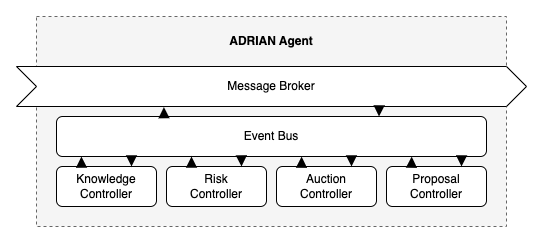
\includegraphics[width=0.8\textwidth]{_content/adrian-component-overview}
    \caption{Agent component overview}
    \label{fig:component-overview}
\end{figure}

\begin{figure}[H]
    \centering
    \includegraphics[width=0.8\textwidth]{_content/knowledge-sharing}
    \caption{Knowledge Exchange Sequence Diagram}
    \label{fig:knowledge-sharing}
\end{figure}


\begin{figure}[H]
    \centering
    \includegraphics[width=1.4\textwidth]{_content/auction}
    \caption{Auction Sequence Diagram}
    \label{fig:auction}
\end{figure}

\section{Future Research}
\label{sec:future-research}

After running the experiments and analyzing the results, we have identified some areas of (potential) improvement in the system. In this section we will discuss some of these areas.

In Section \ref{sssec:knowledge-depth} the concept of knowledge depth was mentioned. As this research kept it at a constant value of 1, it would be interesting to see how this system would perform with different values. This could be done by running the experiments again, but with different values for the knowledge depth. This would give a better understanding of how the knowledge depth affects the performance of the system.

Another area for further research is the risk rules. As mentioned in Section \ref{sssec:risk-rules}, the risk rules are quite simple. It would be interesting to see how the system would perform with more complex risk rules. This could be done by running the experiments again, but with more complex risk rules. This would give a better understanding of how the risk rules affect the performance of the system. 

During the implementation and experimentation some back-and-forth discussions were held about the risk reports that were sent during an auction. The risk reports contain a subsection of the entire attackgraph a node calculated, containing only the nodes that are part of the risk path the auction tries to mitigate. This subsection would contain all risk edges between the nodes, including their probabilities (See figure \ref{fig:riskreport-a}). This would result in a large amount of data being sent during an auction. 

\begin{figure}[H]
    \centering
    \begin{subfigure}[b]{0.4\textwidth}
        \centering
        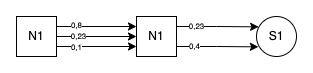
\includegraphics[width=\textwidth]{_content/riskreport-future-research-a.png}
        \caption{Full risk report with all edges.}
        \label{fig:riskreport-a}
    \end{subfigure}
    \hspace{0.5cm}
    \begin{subfigure}[b]{0.4\textwidth}
        \centering
        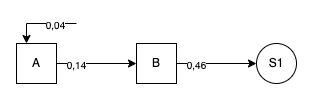
\includegraphics[width=\textwidth]{_content/riskreport-future-research-b.png}
        \caption{Merged risk report with only one edge.}
        \label{fig:riskreport-b}
    \end{subfigure}
    \caption{Two different methods of dealing with risk reports, where on the left all risk edges are present and no information is lost. On the right all risk edges between nodes have been merged into a single edge, resulting in a smaller amount of data being sent.}
\end{figure}


An alternative to sending all edges, was to merge the probabilities of all the edges between two nodes into a single edge (See figure \ref{fig:riskreport-b}). This merging could be done similar to the logic that is used when calculating the risk damage value, for example $p = \prod_{k=1}^{R} (1 - p_{k})$ where $R$ is the risk edges between the nodes, and $p_{k}$ is the probability for an edge. 
This would result in a smaller amount of data being sent during an auction. However, this would also result in a loss of information. Since there are no actual messages sent over the network in the experiments, the amount of data that was sent was not a bottleneck, so the decision was made to send all edges of the subgraph. However, if this system were to be implemented in a real-world scenario, the amount of data sent could be a bottleneck. In that case, it would be interesting to see how the system would perform with the alternative risk report.


\section{Conclusion}
\label{sec:conclusion}

At the start of this research we set out to answer the following research questions:

\vspace{0.5em}
\emph{Can the ADRIAN protocol be implemented and used for effective Risk Assessment and Mitigation?}
\vspace{0.5em}

Which would inturn be answered by the following questions: 
\begin{itemize}
    \item \textit{(Identification) Can we use the ADRIAN protocol to do automated risk identification within a network of nodes with an (imperfect) local knowledge base?}
    \item \textit{(Mitigation) Can the ADRIAN protocol be used to decrease the overall risk, by applying adaptation patterns over time?}
\end{itemize}

In this section we will answer these questions, with the information from the Result and Discussion sections in mind.

\paragraph*{Identification}
In Subsection \ref{ssec:risks-detected} we explained that the full implementation of the ADRIAN protocol is capable of detecting risks in a network of nodes. By using an internal knowledge base agents are able to detect risks that they would otherwise be unable to detect. The benefits of this decentralized approach are that agents only need to store, share, and assess the properties of each node for a subset of the problem. This makes it very scalable and allows for a large number of nodes to be added to the network. However, this also means that the agents are unable to detect risks that are outside of their knowledge base. This is a trade-off that is made in the ADRIAN protocol. 

\paragraph*{Mitigation}
The ADRIAN protocol, even without auctions, is able to decrease the overall risk and predicted damage of an infrastructure.
Subsections \ref{ssec:efficient-adaptations} and \ref{ssec:adaptation-time} explain that the full implementation of the ADRIAN protocol is capable of reducing the overall damage of the infrastructure, by using the concepts of auctions. These auctions allow agents to apply more effective adaptations, and reduce the amount of service-/downtime a node and its software components experience. 


\vspace{0.5em}
Combining all the information from Section \ref{sec:discussion} and the answers to the sub-research questions, we can conclude that the ADRIAN protocol can be used for effective risk assessment and mitigation. 


\bibliographystyle{abbrv}
\bibliography{bibliography}
\end{document}
